% ========================================= TEMPLATE INFO ========================================
%
% Author:       P4ntomime
% Version:      1.0.0
% Last updated: 2024-02-18
% Brief:        A LaTeX template for summaries. See README.md for more information.
% 
% ================================================================================================
\documentclass[8pt, a4paper, twoside, landscape]{extarticle}
% Font size:    8pt
% Paper size:   A4
% style:        twoside (needed, so odd and even pages have different margins)
% orientation:  portrait. (use 'landscape' for landscape orientation)


% ========================================= DOCUMENT INFO =========================================
\def\title{Technikgeschichte}       % title
\def\shorttitle{Technikgeschichte}                            % short title (displayed as PDF title)
\def\dozent{Dr. Mirijam Mayer}               % docent
\def\semester{FS 2026}                              % semester
\def\author{Gian Marco Näf, Laurens Perseus}                           % author(s)
\def\repo{https://github.com/Giamo08/Zusammenfassungen}        % repository link
\def\version{1.0.\today}                            % version
\def\pagelimit{50}                                   % page limit -> causes pages after limit to be red
\def\titleoption{ultra compact}                     % options: ultra compact, compact, normal
\def\enableToC{false}

% ================================= PACKAGES, SETUP AND COMMANDS ==================================
\makeatletter
\def\input@path{{./}{TeGesch/}}
\makeatother
\input{preamble.tex}

\titlespacing*{\section}{0pt}{2.5ex plus 1ex minus .2ex}{3ex plus .5ex}
\makeatletter
\def\@enableToC{true}
\ifx\enableToC\@enableToC
    \setcounter{tocdepth}{2} % adjust depth: 0=parts,1=sections,2=subsections,...
    \AtBeginDocument{%
        \clearpage
        \tableofcontents
        \clearpage
    }
\fi
\makeatother

% =========================================== DOCUMENT ============================================
\begin{document}
    \begin{layout}
        \section{Wozu Technikgeschichte?}

\subsection{Leben in einer technischen Kultur}

Die Vorlesung beginnt mit einem Gedankenexperiment: 
Man soll sich eine Gesellschaft vorstellen, die keinerlei Techniken kennt. 

Bereits nach kurzer Überlegung wird deutlich, dass eine solche Gesellschaft kaum vorstellbar ist. 
Ohne Technik gäbe es weder Elektrizität noch Fahrzeuge, keine Kommunikationsmittel, 
keine Produktionssysteme, keine Werkzeuge, keine Kleidung, keine Behausungen und 
nicht einmal symbolische Systeme wie Schrift oder Zahlen. 

Diese Überlegung führt zu einer zentralen Erkenntnis:

\begin{itemize}
    \item Technik ist kein Zusatz zur Gesellschaft.
    \item Technik ist inhärenter Bestandteil gesellschaftlichen Zusammenlebens.
    \item Technik ist Voraussetzung menschlicher Welterfahrung.
\end{itemize}

Technik ist somit nicht etwas Äusserliches oder Nachgeordnetes, sondern konstitutiv für 
menschliches Handeln, Wahrnehmen und Organisieren.

\subsection{Was ist Gegenstand der Technikgeschichte?}

Technikgeschichte beschäftigt sich nicht primär mit der Frage, 
wer eine bestimmte Maschine erfunden hat oder wie ein technisches System 
im Detail funktioniert. 

Im Zentrum steht vielmehr das Verhältnis zwischen Technik und Gesellschaft. 

Der Technikbegriff wird dabei weit gefasst. Technik umfasst:

\begin{itemize}
    \item Geräte und Maschinen
    \item Infrastrukturen
    \item Fertigkeiten und Praktiken
    \item Formen der Ausführung bestimmter Tätigkeiten
\end{itemize}

Technik ist somit nicht nur ein materielles Objekt, sondern auch eine Praxis.

\subsection{Wechselwirkungen zwischen Technik und Gesellschaft}

Technikgeschichte untersucht zwei grundlegende Fragestellungen:

\begin{enumerate}
    \item Wie verändern Techniken Gesellschaften?
    \item Wie prägen gesellschaftliche Phänomene technische Entwicklungen?
\end{enumerate}

Diese beiden Wirkungsrichtungen lassen sich meist nicht klar voneinander trennen. 
Technik beeinflusst gesellschaftliche Strukturen, während gleichzeitig soziale, 
politische und wirtschaftliche Bedingungen technische Entwicklungen formen.

Es besteht somit ein wechselseitiger Prozess, in dem Technik und Gesellschaft 
untrennbar miteinander verflochten sind.

\subsection{Fallbeispiel: Bau der Fürstenlandbrücke (1937--1941)}

\begin{center}
    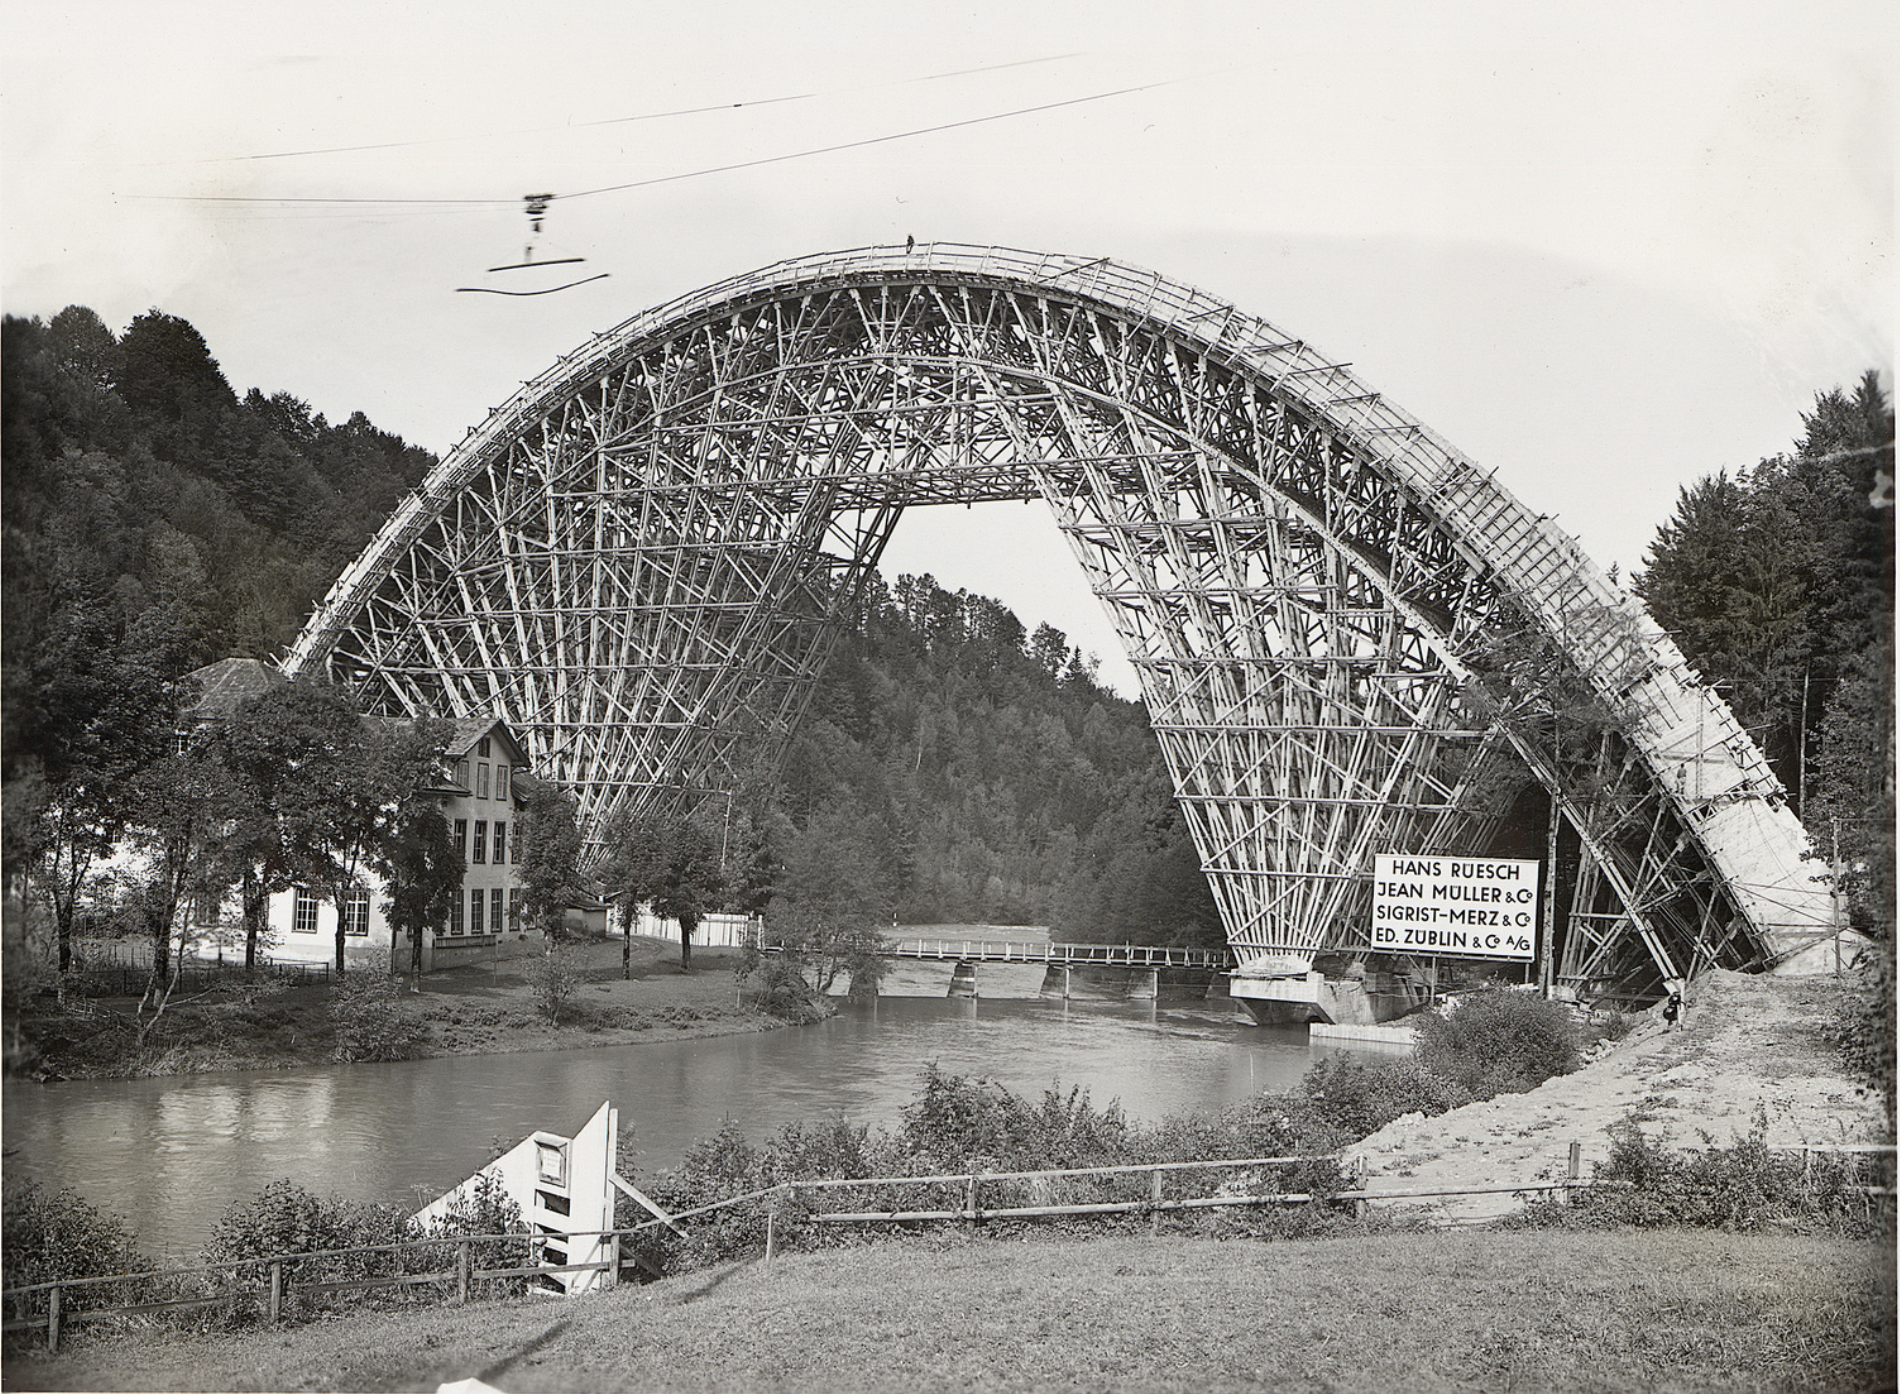
\includegraphics[width=0.8\linewidth]{images/bruecke.png}
\end{center}

Am Beispiel des Baus der Fürstenlandbrücke in St.\ Gallen wird deutlich, 
wie Technik als gesellschaftliches Phänomen analysiert werden kann.

Das Bauwerk war nicht nur eine technische Konstruktion, sondern eingebettet in 
verschiedene gesellschaftliche Kontexte:

\begin{itemize}
    \item \textbf{Mobilität:} Anpassung an neue Verkehrsmittel (Kutsche, Auto, Fahrrad, Fussverkehr).
    \item \textbf{Raumstruktur:} Verbindung von Peripherie und Zentrum durch Überwindung der Sitterschlucht.
    \item \textbf{Modernität:} Ausdruck ingenieurtechnischer Leistungsfähigkeit, Planung, Logistik und Statik.
    \item \textbf{Wirtschaft und Politik:} Arbeitsbeschaffung in einer Phase wirtschaftlicher Umbrüche.
\end{itemize}

Das Beispiel verdeutlicht, dass technische Objekte stets politische, wirtschaftliche, 
kulturelle und symbolische Dimensionen besitzen.

\subsection{Technikgeschichte als Gesellschaftsgeschichte}

Technikgeschichte arbeitet multiperspektivisch. 
Gesellschaften handeln widersprüchlich, weshalb auch technische Entwicklungen 
unterschiedlich interpretiert werden.

Wichtige Einsichten sind:

\begin{itemize}
    \item Technik determiniert ihren Nutzen oder ihre Bedeutung nicht automatisch.
    \item Technik ist nicht neutral.
    \item Akteure deuten Technik unterschiedlich.
\end{itemize}

Unterschiedliche Gruppen (Ingenieur*innen, Politiker*innen, Unternehmen, Nutzer*innen) 
verfolgen divergierende Interessen. 

Gleichzeitig besitzt Technik materielle Eigenschaften, die bestimmte Handlungen 
ermöglichen oder begrenzen. 

Technik ist somit sowohl sozial konstruiert als auch materiell wirksam.

\subsection{Methodisches Vorgehen der Geschichtswissenschaft}

Die historische Analyse beruht auf drei zentralen Elementen:

\begin{itemize}
    \item \textbf{Historische Quelle:} Bilder, Texte, Artefakte, Filme, technische Objekte.
    \item \textbf{Kontext:} Politische, ökonomische, gesellschaftliche und geopolitische Rahmenbedingungen.
    \item \textbf{Narrativ:} Perspektive und Deutung der erzählten Geschichte.
\end{itemize}

Geschichte ist somit nicht nur Rekonstruktion von Fakten, sondern immer auch 
Interpretation und Deutung.

\subsection{Ziel des Kurses}

Der Kurs verfolgt mehrere Zielsetzungen:

\begin{itemize}
    \item Sensibilisierung für die gesellschaftliche Bedeutung technischer Entscheidungen.
    \item Entwicklung historischer Urteilskompetenz.
    \item Förderung der Quellenkritik.
    \item Verständnis langfristiger technischer Entwicklungen.
\end{itemize}

Technikgeschichte soll insbesondere zukünftige Entscheidungsträger*innen 
befähigen, technische Entwicklungen nicht isoliert, sondern in ihren 
gesellschaftlichen Zusammenhängen zu reflektieren.

\subsection{Zusammenfassung}

Die zentrale Aussage der ersten Sitzung lautet:

Technik ist kein externer Faktor der Gesellschaft, sondern konstitutiver Bestandteil 
menschlicher Existenz. 

Technikgeschichte analysiert daher:

\begin{itemize}
    \item Die Wechselwirkung zwischen Technik und Gesellschaft,
    \item Die gesellschaftliche Einbettung technischer Entwicklungen,
    \item Die Deutung und Bedeutung technischer Artefakte,
    \item Die langfristigen Wirkungen technischer Entscheidungen.
\end{itemize}

Das Fach vermittelt somit nicht nur historisches Wissen, sondern 
eine reflektierte Perspektive auf die Rolle von Technik in Vergangenheit, 
Gegenwart und Zukunft.
        \section{Wie die Welt in den Computer kam – Narrative der Technikgeschichte}

\subsection{Einführung: Computergeschichte als Erzählung}

Die Sitzung beginnt mit einer populären Computergeschichte (Film). 
Bereits hier wird deutlich: Computergeschichte ist nie nur eine Abfolge technischer Innovationen, 
sondern immer auch eine \textit{Erzählung}.

Zentrale Leitfragen:

\begin{itemize}
    \item Was wird erzählt – und was wird nicht erzählt?
    \item Wer erscheint als Erfinderfigur?
    \item Welches Problem soll der Computer lösen?
    \item Was ist überhaupt ein Computer?
\end{itemize}

Computergeschichte ist somit nicht neutral, sondern konstruiert Bedeutungen, 
setzt Schwerpunkte und lässt andere Aspekte verschwinden.

\subsection{Etappen der Computergeschichte}

Die Vorlesung strukturiert die Geschichte des Computers in fünf Phasen:

\begin{enumerate}
    \item Vorläufer bis 1900
    \item 1930er/1940er: Militär und Wissenschaft
    \item 1950er/1960er: Kommerzielle Verwaltungsmaschinen
    \item 1970er/1980er: Computer für alle
    \item Ab 1990: Computer als Infrastruktur und Umwelt
\end{enumerate}

Diese Periodisierung zeigt, dass sich nicht nur die Technik, sondern auch 
die gesellschaftliche Funktion des Computers verändert.

\subsection{1. Vorläufer bis 1900}

\begin{center}
    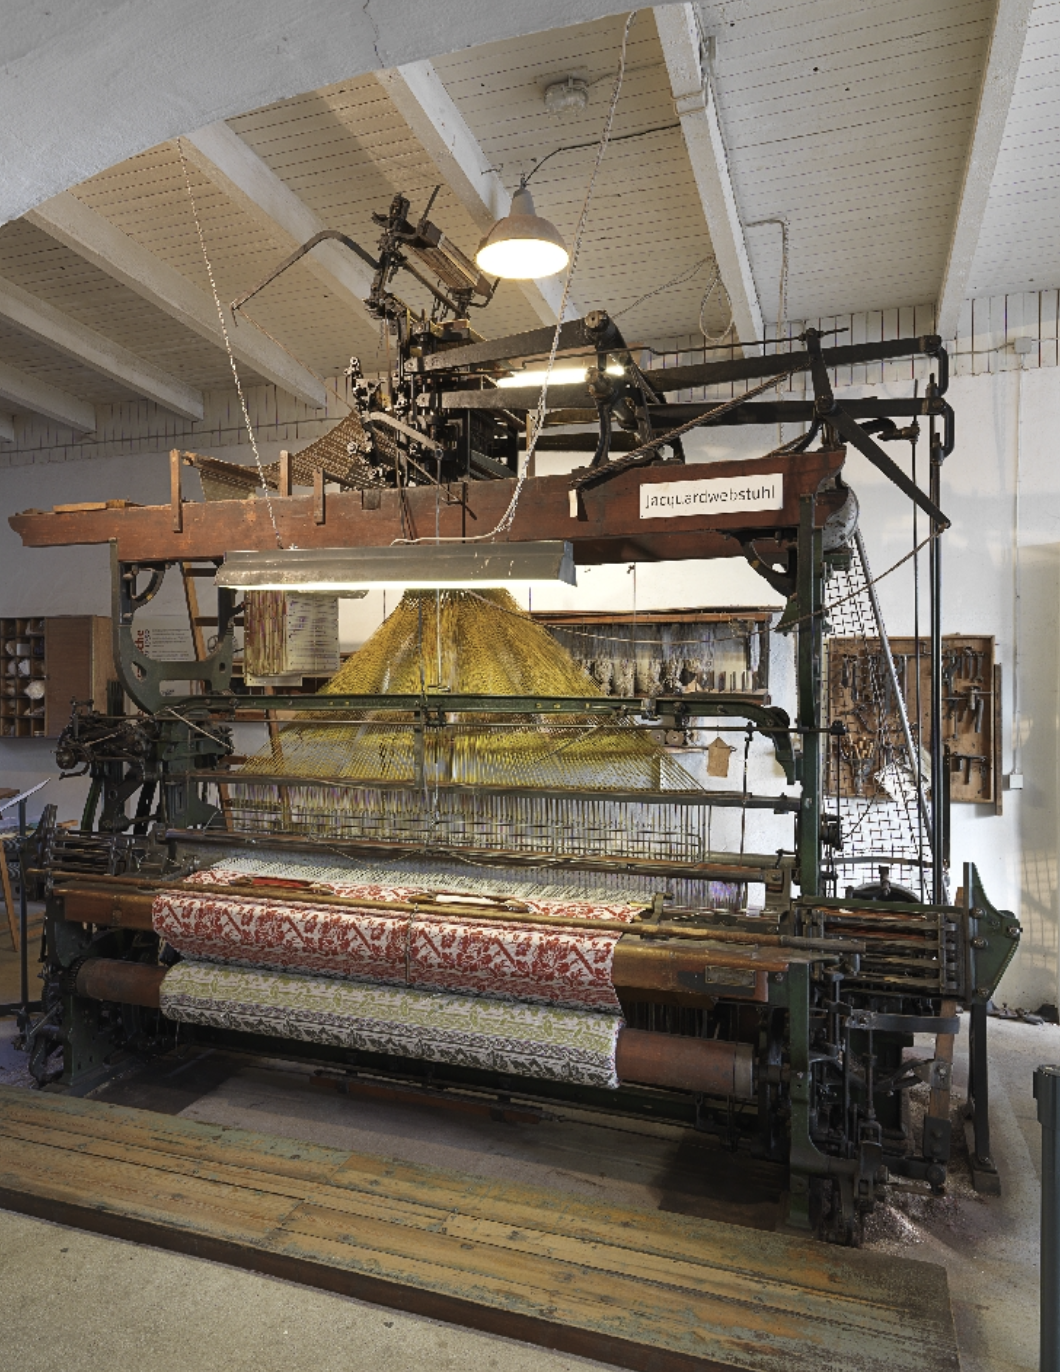
\includegraphics[width=0.8\linewidth]{images/jacquardwebstuhl.png}
\end{center}

\begin{center}
    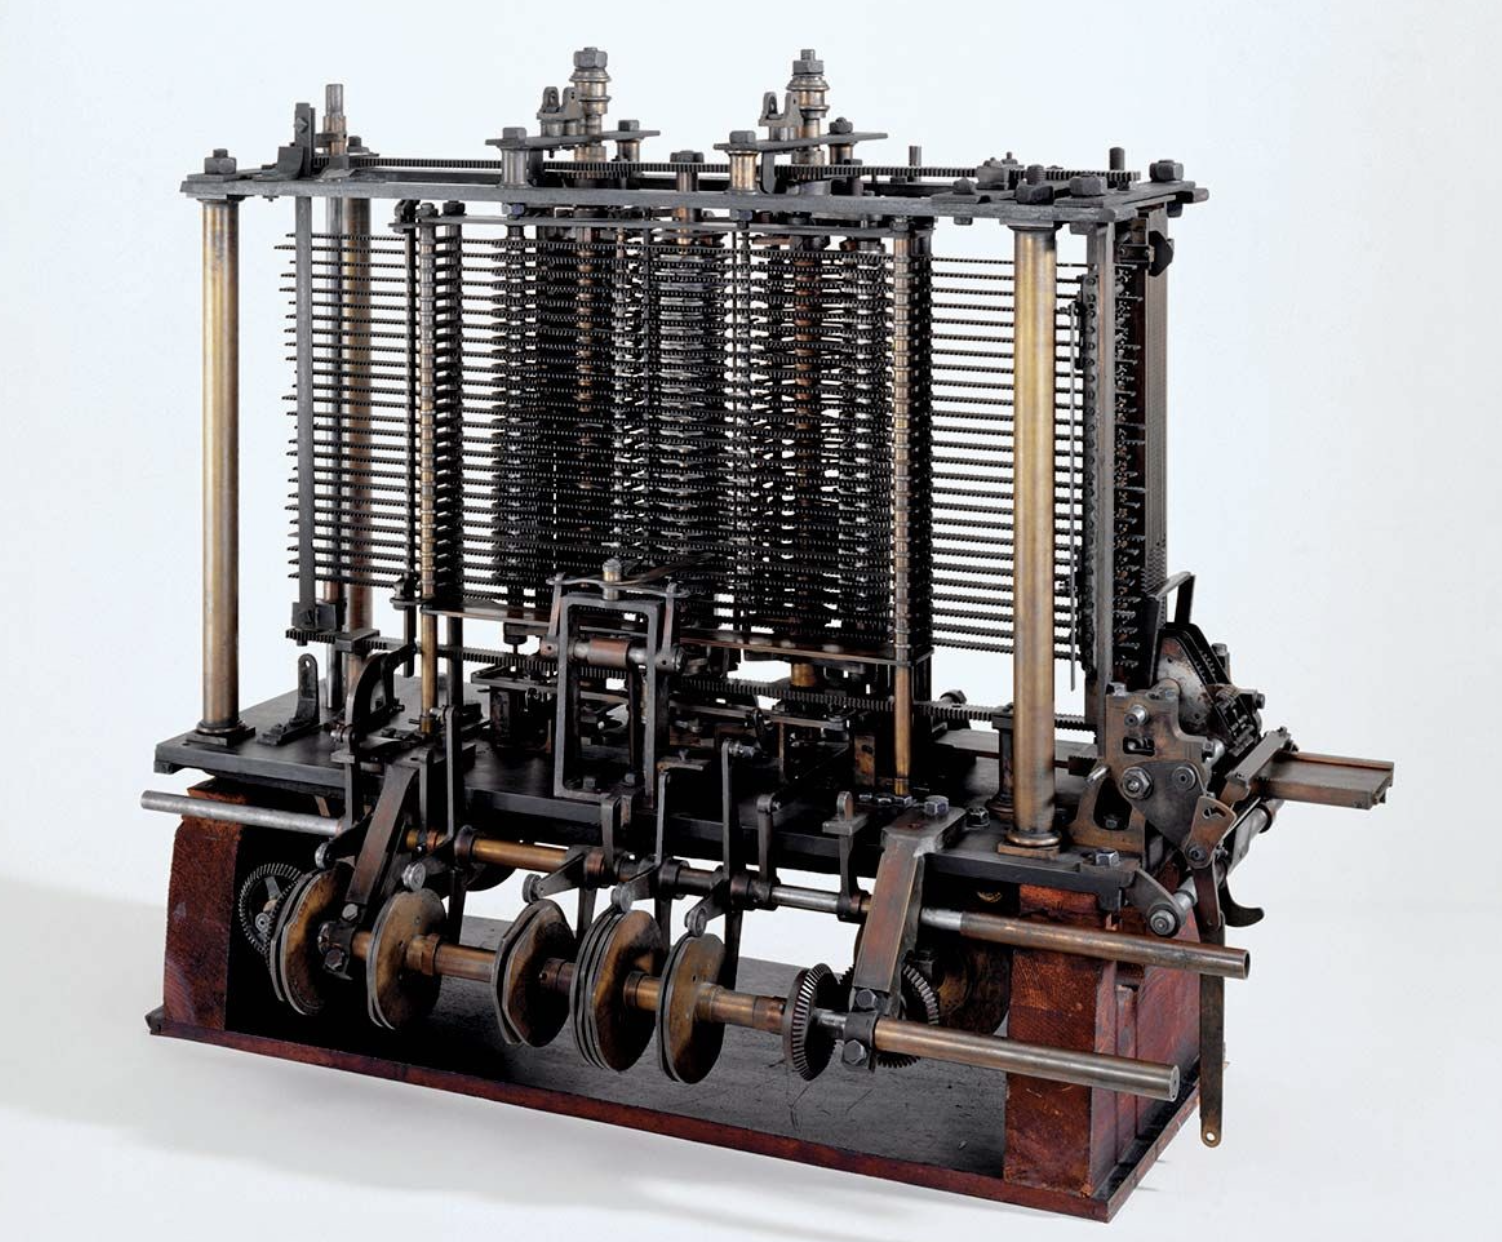
\includegraphics[width=0.8\linewidth]{images/analyticalmachine.png}
\end{center}

Die frühen Vorläufer waren keine „Computer“ im heutigen Sinn, 
sondern Maschinen zur Automatisierung bestimmter Prozesse.

\paragraph{Jacquardwebstuhl (um 1800)}

\begin{itemize}
    \item Automatisierung komplexer Webmuster
    \item Steuerung über Lochkarten
    \item Industrielle Anwendung
\end{itemize}

Hier wird erstmals das Prinzip sichtbar, dass ein Programm 
von der Maschine getrennt existieren kann.

\paragraph{Analytical Machine (Babbage/Lovelace, 1840er)}

\begin{itemize}
    \item Dampfbetrieben
    \item Lochkarten
    \item Allgemeine Programmierbarkeit
    \item Theoretisches Konzept, nicht realisiert
\end{itemize}

Die Analytical Machine formulierte bereits das Prinzip eines 
universellen Rechners.

\paragraph{Hollerith-Maschinen (um 1900)}

\begin{itemize}
    \item Lochkartenbasiert
    \item Verarbeitung grosser Datenmengen
    \item Einsatz bei Volkszählungen
    \item Verwaltungsmaschine
\end{itemize}

Hier verschiebt sich der Zweck: weg von mathematischen Problemen, 
hin zur Datenverarbeitung im administrativen Kontext.

Gemeinsames Prinzip dieser Vorläufer:
Die Trennung von Maschine und Programm ermöglicht 
eine Zweckungebundenheit des Rechners.

\subsection{2. 1930er und 1940er: Militär und Wissenschaft}

Mit der Elektrifizierung entstehen elektronische und elektromechanische Rechner.

Beispiele:

\begin{itemize}
    \item Konrad Zuse (Z4)
    \item Colossus (Grossbritannien)
    \item ENIAC (USA)
\end{itemize}

Der Computer wird zur Kriegstechnologie.

Zwecke:

\begin{itemize}
    \item Ballistische Berechnungen
    \item Kryptographie
    \item Entwicklung der Atombombe
\end{itemize}

Charakteristisch:

\begin{itemize}
    \item Massive staatliche Investitionen
    \item Geheimhaltung
    \item Nationale Sicherheit als Legitimation
\end{itemize}

Der Computer ist nun strategisches Instrument.

\subsection{3. 1950er/1960er: Kommerzielle Verwaltungsmaschinen}

\begin{center}
    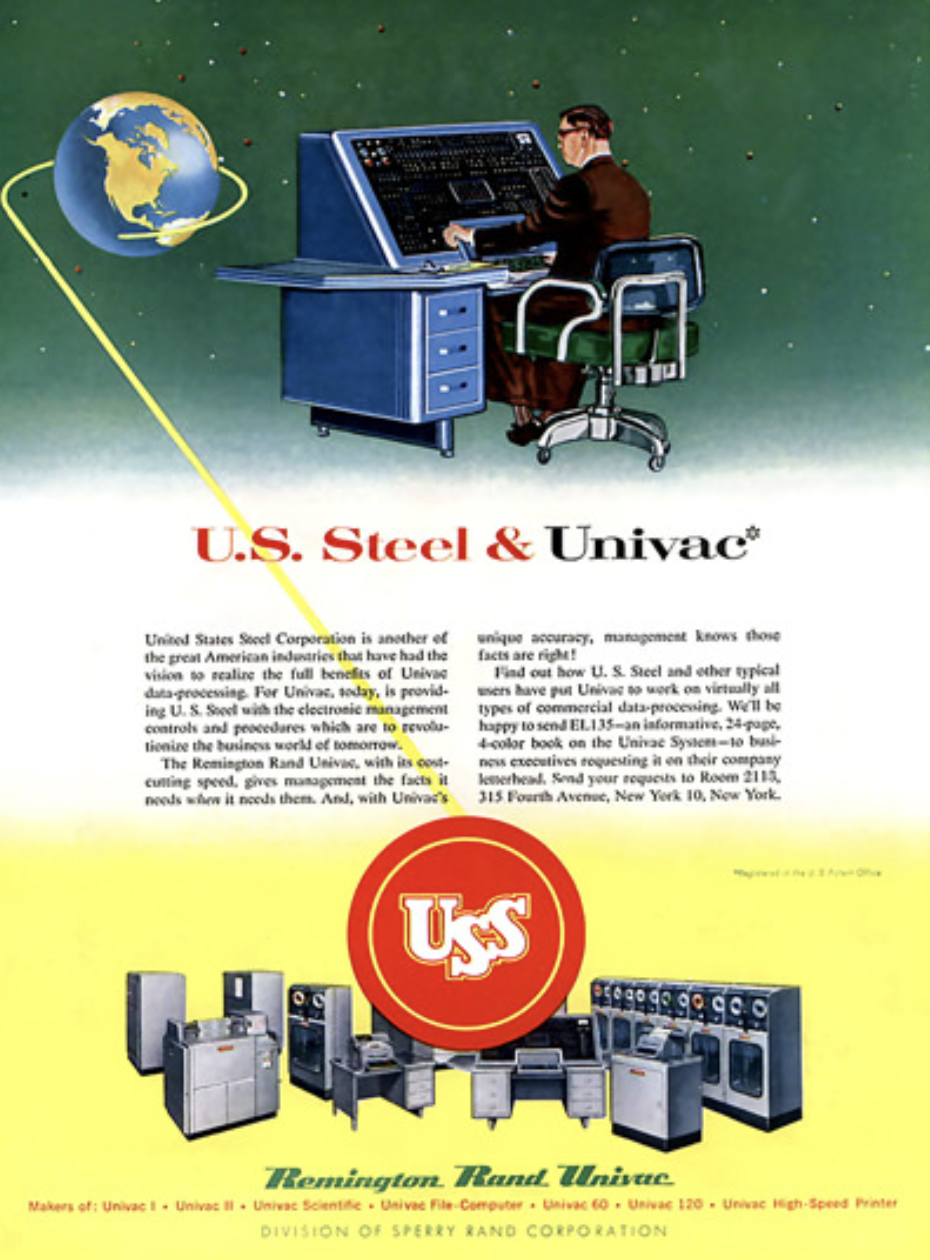
\includegraphics[width=0.8\linewidth]{images/univacwerbung.png}
\end{center}

Mit UNIVAC (1951) beginnt die kommerzielle Phase.

\paragraph{Mainframes}

\begin{itemize}
    \item Raumfüllende Grossrechner
    \item Installation in Rechenzentren
    \item Nutzung durch Banken, Versicherungen, Verwaltungen
\end{itemize}

Zweck:
Effizienzsteigerung bürokratischer Prozesse.

\paragraph{Datenverarbeitung}

Der Prozess war komplex:

\begin{enumerate}
    \item Daten erfassen (Digitalisierung)
    \item Programm schreiben
    \item Lochkarten stanzen
    \item Im Rechenzentrum einreichen
    \item Warten (Stapelverarbeitung)
    \item Resultate abholen
\end{enumerate}

Probleme:

\begin{itemize}
    \item Hohe Kosten
    \item Vermeidung von „idle time“
    \item Unflexible Stapelverarbeitung
\end{itemize}

\paragraph{Technische Lösungen}

\begin{itemize}
    \item Random Access (Magnetplatten statt Magnetband)
    \item Time-Sharing (Mehrere Terminals, quasi Echtzeit)
\end{itemize}

Folgen:

\begin{itemize}
    \item Flexibilisierung des Datenzugriffs
    \item Grundlage für Datenbanksysteme
    \item Beginn der Vernetzung
\end{itemize}

\subsection{4. 1970er/1980er: Computer für alle}

Mit dem Mikroprozessor werden Computer kleiner, billiger und leistungsfähiger.

Es entstehen:

\begin{itemize}
    \item Personal Computer
    \item Vernetzungstechnologien
    \item Neue Firmen im Silicon Valley
\end{itemize}

Die Erzählung ändert sich:
Computer werden als Mittel zur Demokratisierung inszeniert.

Gleichzeitig:

\begin{itemize}
    \item Standardsoftware reguliert Nutzungsmöglichkeiten
    \item Benutzeroberflächen verdecken technische Komplexität
\end{itemize}

Hackerkulturen (z.B. Chaos Computer Club) reagieren kritisch und fordern 
Datenschutz und Transparenz.

Technik tritt zunehmend in den Hintergrund.

\subsection{5. Ab 1990: Computer als Infrastruktur und Umwelt}

Mit dem Internet verschwindet der Computer als einzelnes Gerät 
und wird Teil einer globalen Infrastruktur.

\begin{itemize}
    \item Tim Berners-Lee entwickelt das World Wide Web
    \item Browser (Mosaic, Netscape) machen es zugänglich
    \item Suchmaschinen strukturieren Daten
\end{itemize}

Neu ist:

\begin{itemize}
    \item Verkauf digitaler Dienstleistungen
    \item Plattformökonomie (Amazon, Google, Facebook)
    \item Daten als Zahlungsmittel
\end{itemize}

Der Computer wird unsichtbar – er wird zur Umwelt.

Zentrale Frage:
Was ist ein Computer noch, wenn er überall ist?

\subsection{Zentrale Erkenntnisse}

Die Geschichte des Computers ist keine lineare Erfolgsgeschichte.

Sie zeigt:

\begin{itemize}
    \item Verschiebung der Zwecke (Rechnen → Verwaltung → Kommunikation → Infrastruktur)
    \item Veränderung der Akteurskonstellationen (Privatpersonen → Militär → Konzerne → Plattformen)
    \item Wandel der Wahrnehmung (sichtbare Maschine → unsichtbare Infrastruktur)
\end{itemize}

Computergeschichte ist daher immer auch:

\begin{itemize}
    \item Militärgeschichte
    \item Verwaltungsgeschichte
    \item Wirtschaftsgeschichte
    \item Kulturgeschichte
    \item Infrastrukturgeschichte
\end{itemize}

Die zentrale These lautet:

Nicht nur der Computer hat sich verändert – 
auch das, was als „Computer“ gilt, hat sich historisch gewandelt.

        \section{Technik als Deutungsangebot – Raketentechnik und Raumfahrt}

\subsection{Einführung: Technik als historisches Deutungsangebot}

Die Vorlesung betrachtet Raketentechnik nicht primär als technische Entwicklung,
sondern als historisches und gesellschaftliches Deutungsangebot.

Technik besitzt keine feste Bedeutung.
Je nach historischem Kontext kann dieselbe Technologie unterschiedliche Funktionen,
Ziele und Symboliken erhalten.

Zentrale Leitfragen:

\begin{itemize}
    \item Welche Bedeutungen werden Raketen zugeschrieben?
    \item Welche Rolle spielt Krieg bei technischen Innovationen?
    \item Wie verändert sich die Wahrnehmung von Raumfahrt im Laufe der Zeit?
    \item Welche politischen und gesellschaftlichen Interessen prägen technische Entwicklungen?
\end{itemize}

Die Geschichte der Raumfahrt ist daher nicht nur Technikgeschichte,
sondern auch Politik-, Militär- und Kulturgeschichte.

\subsection{Historische Perspektive und Anachronismus}

Zu Beginn wird vor einer häufigen Falle historischer Betrachtung gewarnt:
dem Anachronismus.

Historische Ereignisse werden oft aus heutiger Perspektive bewertet.
Für eine wissenschaftliche Analyse ist jedoch entscheidend, die Sichtweise
der damaligen Akteure und ihren historischen Kontext zu berücksichtigen.

Vergangene Entscheidungen dürfen daher nicht anhand späterer Entwicklungen
oder heutigen Wissens beurteilt werden.

\subsection{Grundlagen der Raketentechnik}

Die technischen Grundprinzipien der Rakete sind erstaunlich konstant geblieben.

Bereits im China des 13. Jahrhunderts wurden Raketen nach dem Rückstossprinzip eingesetzt.

Historisch verändert haben sich jedoch:

\begin{itemize}
    \item Materialien (Stahl, Titan, Nickellegierungen, Carbon)
    \item Antriebssysteme (Feststoff-, Flüssig- und Methantriebwerke)
    \item Steuerungssysteme (digitale Navigation seit den Apollo-Missionen)
    \item Einsatzgebiete und Zwecke
\end{itemize}

Die gleiche Grundtechnologie kann als Waffe,
Trägerrakete, Satellitensystem oder Raumfahrzeug dienen.

\subsection{Technik und Krieg: Die A4 bzw. V2-Rakete}

Ein entscheidender Entwicklungsschritt erfolgte im Zweiten Weltkrieg.

Die Aggregat 4 (A4), später als V2 („Vergeltungswaffe 2“) bezeichnet,
gilt als erste funktionsfähige Fernrakete.

Wichtige Eckpunkte:

\begin{itemize}
    \item Entwicklung unter Wernher von Braun ab 1939
    \item Erste erfolgreiche Tests 1942
    \item Serienproduktion ab 1943
    \item Einsatz gegen Städte wie London und Antwerpen
\end{itemize}

Die Produktion erfolgte in grossen Teilen durch KZ-Häftlinge.
Tausende Menschen wurden zur Arbeit gezwungen,
viele verloren dabei ihr Leben.

Die Geschichte der Rakete ist daher untrennbar mit
nationalsozialistischer Gewalt und Zwangsarbeit verbunden.

\begin{center}
    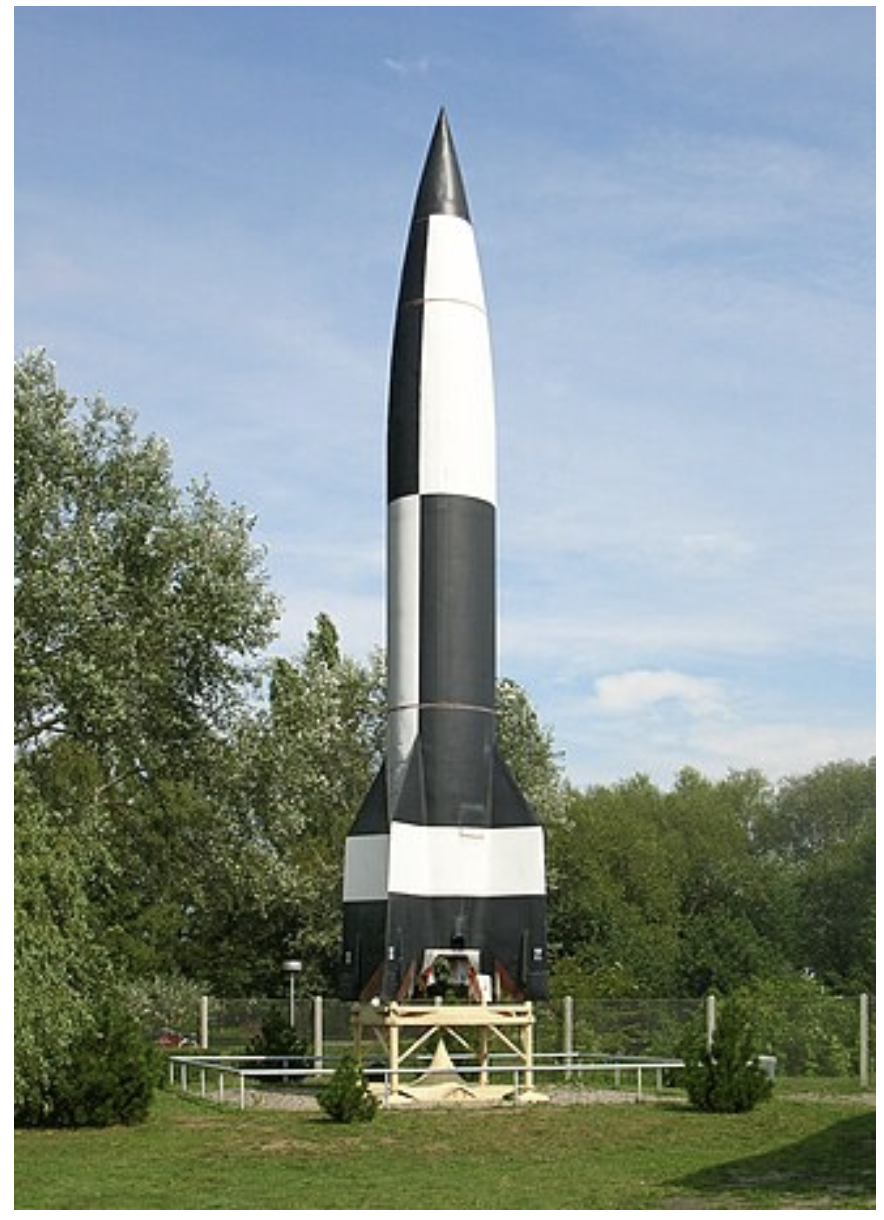
\includegraphics[width=0.8\linewidth]{images/rakete.png}
\end{center}


\subsection{Krieg als Motor technischer Entwicklung?}

Die Vorlesung diskutiert die verbreitete These,
dass Kriege technische Innovationen beschleunigen.

Argumente dafür:

\begin{itemize}
    \item Enorme finanzielle Ressourcen
    \item Enge Zusammenarbeit zwischen Militär, Wissenschaft und Industrie
    \item Hohe politische Priorität
\end{itemize}

Gleichzeitig zeigt sich, dass Krieg Innovationen auch behindern kann:

\begin{itemize}
    \item Geheimhaltung verhindert Wissensaustausch
    \item Fehlender Kostendruck reduziert Effizienz
    \item Produktion und Weiterentwicklung konkurrieren miteinander
    \item Ethische Folgen werden ausgeblendet
\end{itemize}

Die Vorstellung, Krieg sei automatisch ein Innovationstreiber,
wird daher kritisch hinterfragt.

\subsection{Techniker nach dem Zweiten Weltkrieg}

\begin{center}
    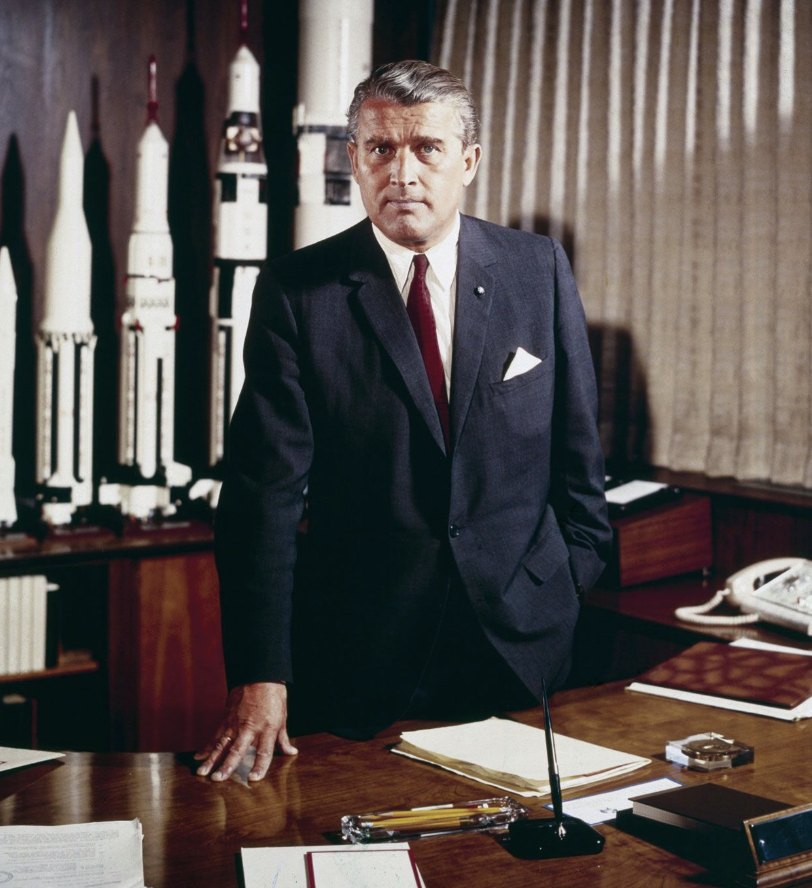
\includegraphics[width=0.8\linewidth]{images/von_Braun.png}
\end{center}

Nach Kriegsende versuchten die Siegermächte,
deutsches Raketenwissen für sich zu nutzen.

Die wichtigsten Programme waren:

\paragraph{Project Paperclip}

Die USA rekrutierten hunderte deutsche Wissenschaftler,
darunter Wernher von Braun.

Viele von ihnen arbeiteten später an den amerikanischen
Raumfahrtprogrammen und den Saturn-Raketen der NASA.

\paragraph{Aktion Ossawakim}

Die Sowjetunion überführte ebenfalls zahlreiche deutsche Spezialisten
in die UdSSR, teilweise freiwillig,
teilweise unter erheblichem Druck.

Damit wurde die deutsche Raketentechnik zu einer wichtigen Grundlage
des späteren Wettlaufs ins All.

\textbf{Bild einfügen:}
Wernher von Braun (wie auf Folie 10).

\subsection{Raumfahrt im Kalten Krieg}

\begin{center}
    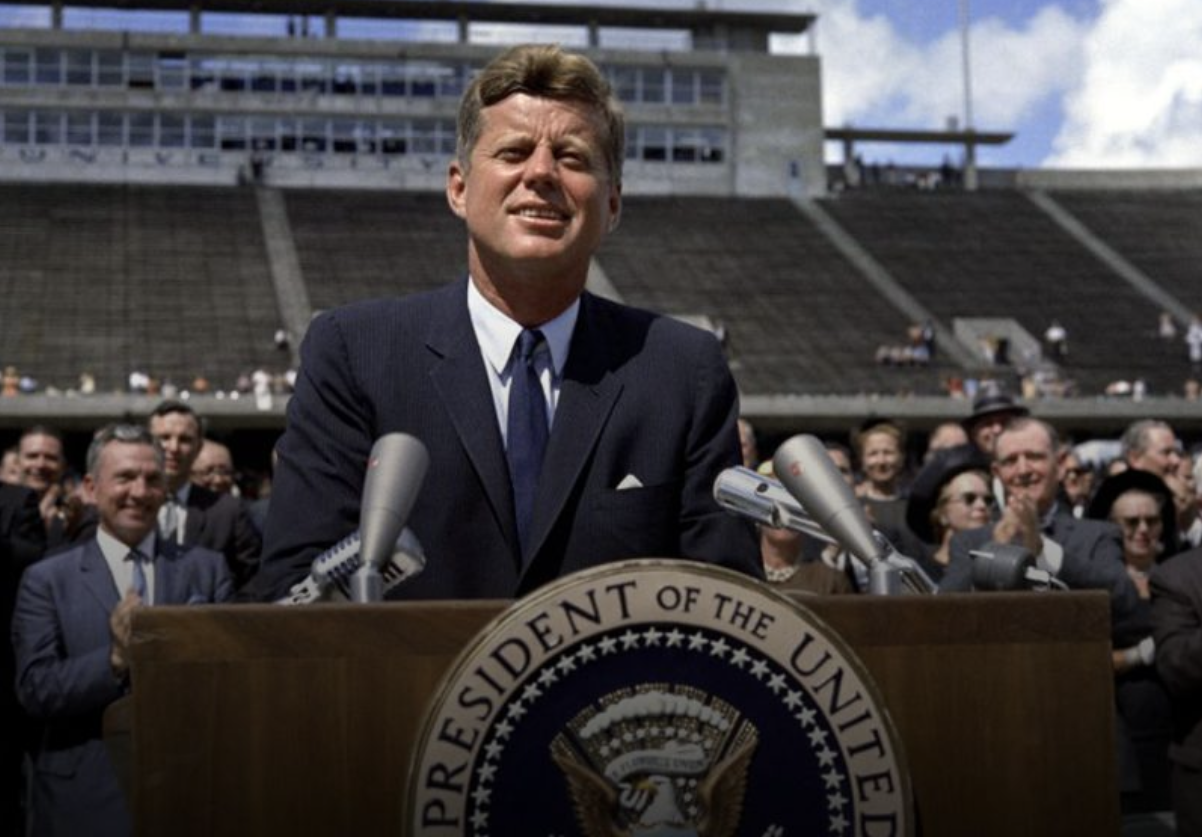
\includegraphics[width=0.8\linewidth]{images/JFK.png}
\end{center}

Im Kalten Krieg wurde Raumfahrt zu einem Symbol
gesellschaftlicher und technologischer Überlegenheit.

Die USA und die Sowjetunion konkurrierten nicht nur militärisch,
sondern auch auf wissenschaftlicher und symbolischer Ebene.

Wichtige Ereignisse:

\begin{itemize}
    \item 1957: Sputnik-Schock
    \item Gründung der NASA
    \item 1961: Juri Gagarin als erster Mensch im Weltall
    \item 1969: Mondlandung der Apollo-11-Mission
\end{itemize}

Raumfahrt wurde zu einem globalen Medienereignis
und zum sichtbaren Ausdruck nationaler Leistungsfähigkeit.

\paragraph{John F. Kennedys Mondrede}

Die Rede „We choose to go to the moon“ von 1962
verdeutlicht, wie politische Akteure technische Projekte legitimieren.

Die Quelle zeigt:

\begin{itemize}
    \item Raumfahrt als nationales Gemeinschaftsprojekt
    \item Betonung von Fortschritt und Pioniergeist
    \item Demonstration amerikanischer Stärke
\end{itemize}

Quellenkritisch ist dabei wichtig,
nicht nur auf den Inhalt,
sondern auch auf Kontext, Publikum und politische Ziele zu achten.

\subsection{Die Neuorientierung der NASA}

Nach der erfolgreichen Mondlandung verlor die NASA
ihr zentrales Ziel des Space Race.

Neue Vorschläge waren:

\begin{itemize}
    \item Bemannte Marsmissionen
    \item Dauerhafte Mondbasis
    \item Ausbau von Satellitenanwendungen
    \item Raumstationen
    \item Wiederverwendbare Raumfahrzeuge
    \item Internationale Kooperation
\end{itemize}

Präsident Richard Nixon reduzierte jedoch das Budget deutlich.

Dadurch verlagerte sich der Schwerpunkt
von spektakulären Einzelmissionen
hin zu langfristiger Infrastruktur.

\subsection{Raumfahrt seit den 1970er Jahren}

Die Raumfahrt entwickelt sich zunehmend
von einem Prestigeprojekt zu einer dauerhaften Infrastruktur.

Wichtige Entwicklungen:

\begin{itemize}
    \item Skylab (1973–1974)
    \item Apollo-Soyuz-Testprojekt (1975)
    \item Internationale Raumstation ISS
    \item Robotische Planetenerkundung
    \item Internationale Zusammenarbeit
\end{itemize}

Seit den 1990er Jahren gewinnen zudem private Unternehmen
an Bedeutung.

Beispiele:

\begin{itemize}
    \item Arianespace
    \item SpaceX
    \item weitere kommerzielle Raumfahrtanbieter
\end{itemize}

\subsection{Neue Raumfahrt im 21. Jahrhundert}

Seit den 2020er Jahren erleben viele frühere Visionen
eine Renaissance.

Diskutierte Projekte:

\begin{itemize}
    \item Dauerhafte Mondbasis
    \item Ressourcenabbau auf dem Mond
    \item Bemannte Marsmissionen
    \item Weltraumtourismus
\end{itemize}

Gleichzeitig entsteht ein neues geopolitisches Konkurrenzverhältnis,
insbesondere zwischen den USA und China.

Die Raumfahrt wird erneut zum Schauplatz
internationaler Machtpolitik.

\subsection{Satelliten als unsichtbare Infrastruktur}

\begin{center}
    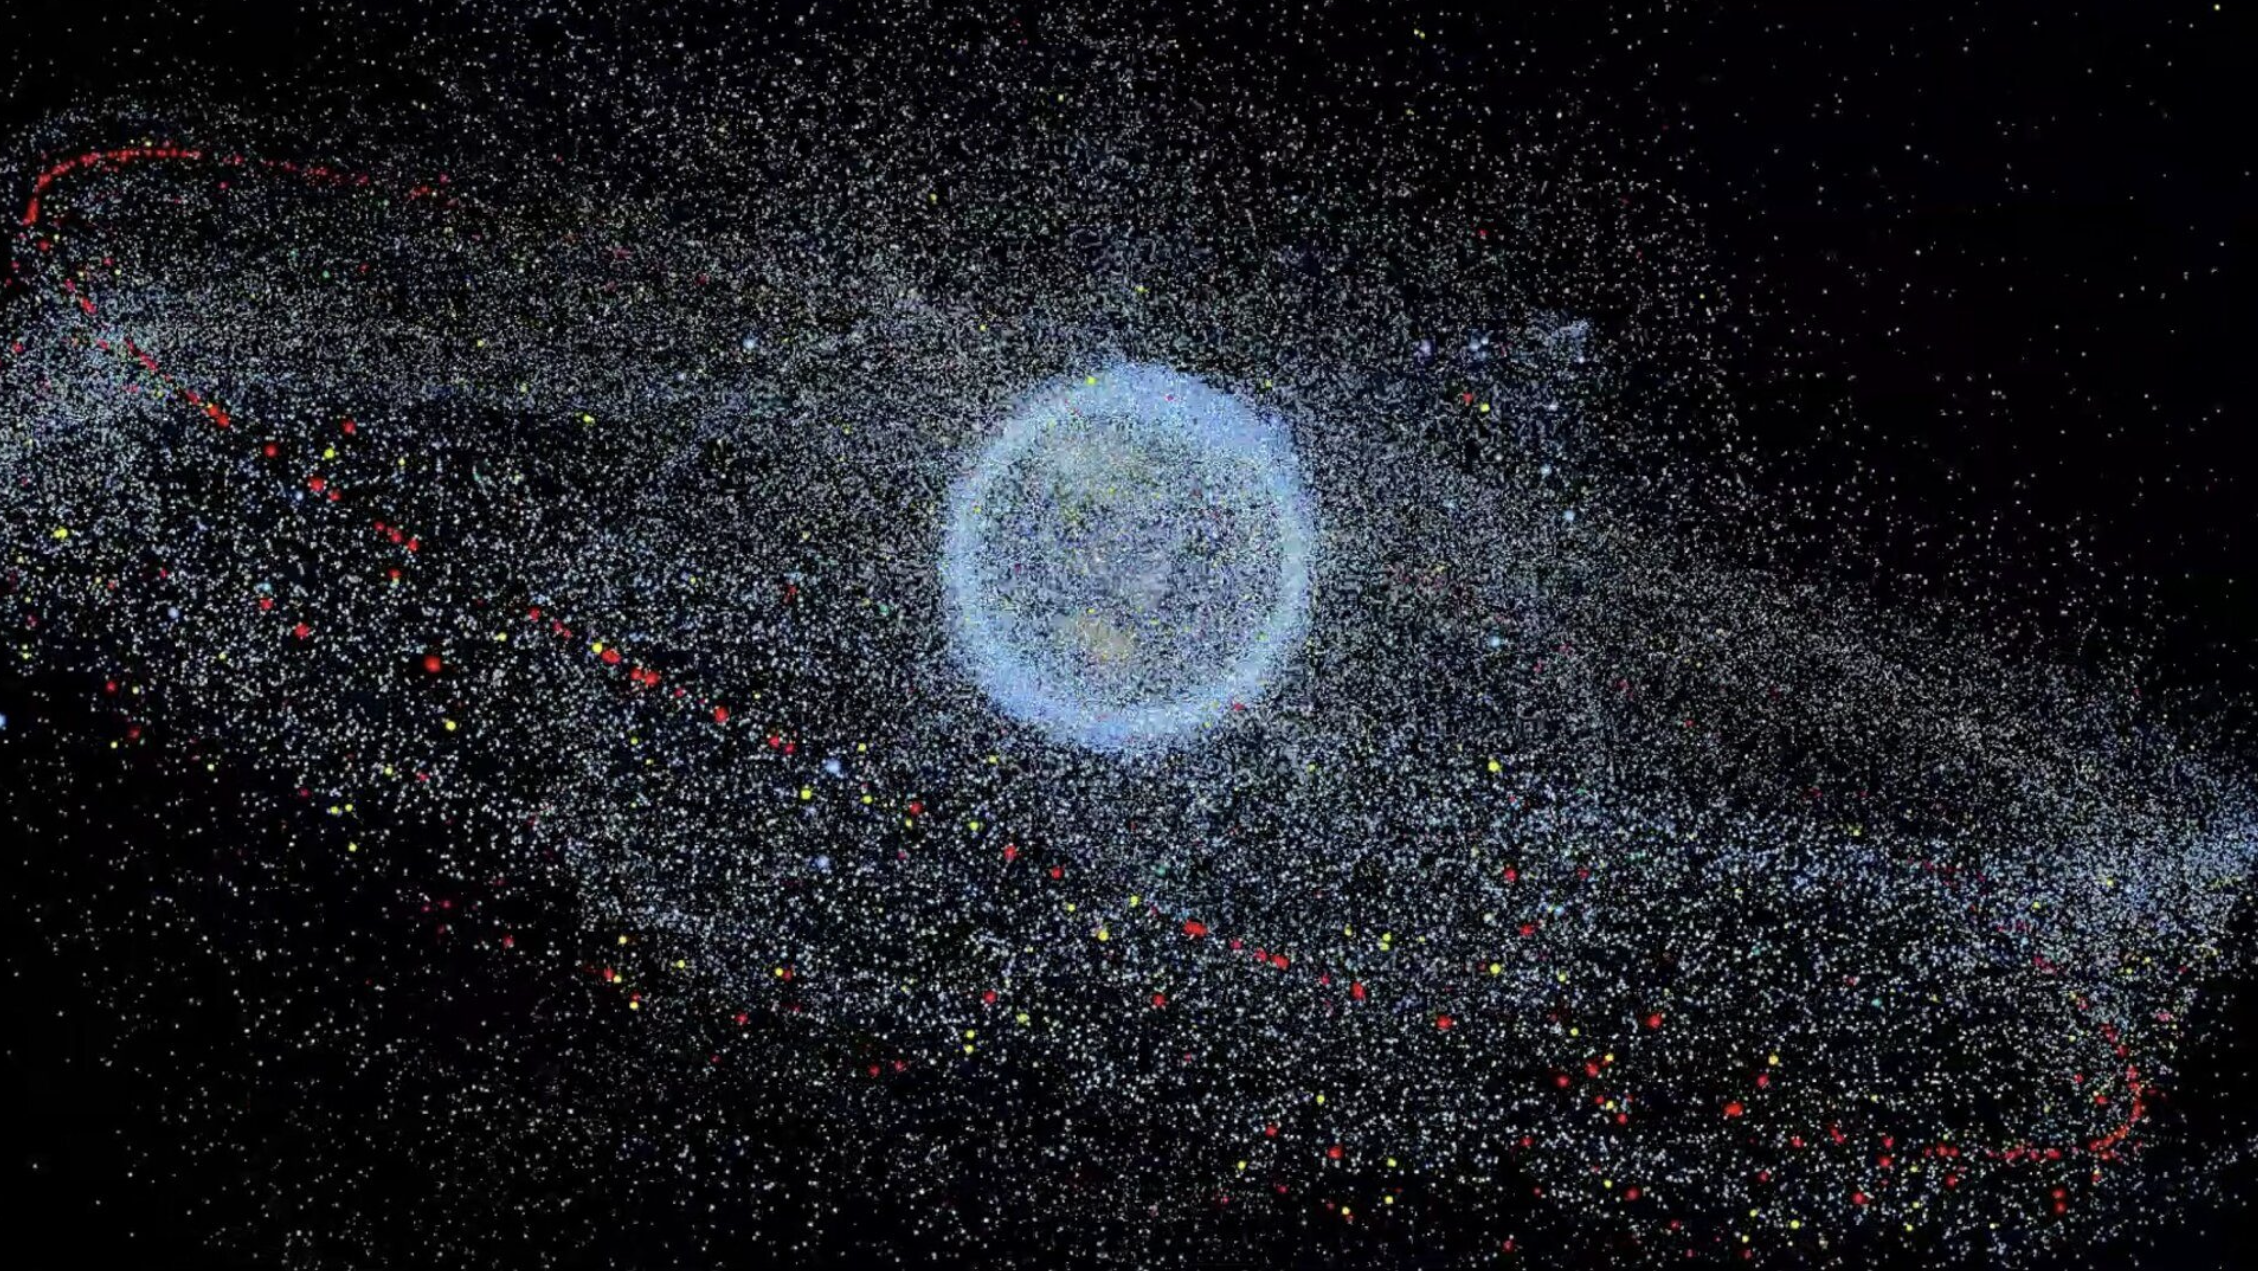
\includegraphics[width=0.8\linewidth]{images/All.png}
\end{center}

Heute prägen vor allem Satelliten den Alltag.

Sie ermöglichen:

\begin{itemize}
    \item Kommunikation
    \item Navigation
    \item Wettervorhersagen
    \item Erdbeobachtung
    \item globale Vernetzung
\end{itemize}

Mit dem Ausbau der Satelliteninfrastruktur
entsteht jedoch auch das Problem des Weltraumschrotts.

Raumfahrt wird dadurch zunehmend zu einer Frage
der nachhaltigen Nutzung orbitaler Infrastrukturen.

\subsection{Zentrale Erkenntnisse}

Die Geschichte der Raketentechnik ist keine reine Erfolgsgeschichte
technischer Innovation.

Sie zeigt:

\begin{itemize}
    \item Die enge Verbindung von Technik und Krieg
    \item Die politische Instrumentalisierung technischer Projekte
    \item Die Bedeutung symbolischer Macht im Kalten Krieg
    \item Die Entwicklung von spektakulären Missionen hin zu Infrastruktur
    \item Die zunehmende Rolle privater Akteure
\end{itemize}

Die zentrale These lautet:

Raketentechnik und Raumfahrt sind nicht nur technische Entwicklungen,
sondern gesellschaftliche Deutungsangebote.
Ihre Bedeutung verändert sich mit den politischen,
wirtschaftlichen und kulturellen Kontexten, in denen sie eingesetzt werden.
        \section{Industrialisierung und Aufbruch in die Moderne}

\subsection{Einführung: Industrialisierung als gesellschaftlicher Transformationsprozess}

Die Vorlesung betrachtet die Industrialisierung nicht nur als technische Entwicklung,
sondern als umfassenden gesellschaftlichen Wandel.

Industrialisierung bezeichnet jene Phase der wirtschaftlichen Entwicklung,
in der industrielle Produktion zur wichtigsten Triebkraft von Wachstum,
Innovation und gesellschaftlicher Veränderung wurde.

Dabei entstanden neue Technologien, Produktionsformen und Wirtschaftsstrukturen,
während traditionelle Formen der Herstellung und Arbeit an Bedeutung verloren. Gleichzeitig veränderten sich Lebensweisen, soziale Beziehungen und politische Verhältnisse grundlegend.

Zentrale Leitfragen:

\begin{itemize}
    \item Was versteht man unter Industrialisierung?
    \item Welche technischen und wirtschaftlichen Entwicklungen ermöglichten sie?
    \item Wie veränderte sich die Arbeitswelt?
    \item Welche gesellschaftlichen Folgen hatte die Industrialisierung?
\end{itemize}

Die Geschichte der Industrialisierung ist daher nicht nur Wirtschafts- und Technikgeschichte,
sondern auch Sozial-, Kultur- und Politikgeschichte.

\subsection{Das historiographische Problem der Industrialisierung}

Die Vorlesung betont, dass Industrialisierung kein einheitlicher Prozess war.

Vielmehr handelt es sich um eine komplexe Entwicklung,
die unterschiedliche Bereiche des gesellschaftlichen Lebens erfasste:

\begin{itemize}
    \item Produktionssysteme
    \item Technologien
    \item Ausbildung und Wissen
    \item Landschaften und Städte
    \item Arbeits- und Lebensweisen
\end{itemize}

Hinzu kommen erhebliche regionale Unterschiede.

Während manche Regionen bereits im 18. Jahrhundert industrialisiert wurden,
erlebten andere diesen Wandel erst deutlich später.

Auch die Perspektive der betrachteten Akteure beeinflusst die historische Darstellung:

\begin{itemize}
    \item Unternehmer
    \item Arbeiterinnen und Arbeiter
    \item Techniker
    \item Fabrikbesitzer
    \item Frauen und Kinder
    \item staatliche Kontrolleure
\end{itemize}

Die Industrialisierung lässt sich deshalb nicht auf eine einzige Ursache zurückführen.
Vielmehr wirkten wirtschaftliche, technische, politische und soziale Faktoren zusammen und beeinflussten sich gegenseitig.

\subsection{Protoindustrie im ostschweizerischen Textilgewerbe}

Vor der eigentlichen Industrialisierung existierten bereits arbeitsteilige Produktionsformen.

Besonders wichtig war in der Ostschweiz zwischen dem 16. und 18. Jahrhundert
das Leinwand- und Baumwollgewerbe.

Kennzeichnend waren:

\begin{itemize}
    \item Verarbeitung von Leinwand und Baumwolle
    \item Einbindung in weltweite Handelsnetzwerke
    \item starke Bedeutung des Zunftwesens
    \item arbeitsteilige Organisation der Produktion
\end{itemize}

Die Herstellung von Textilien erfolgte in zahlreichen einzelnen Arbeitsschritten,
die auf verschiedene Personen und Orte verteilt waren.

Dadurch entstand bereits vor der Industrialisierung eine komplexe Produktionsstruktur,
die als Protoindustrie bezeichnet wird.

\begin{center}
    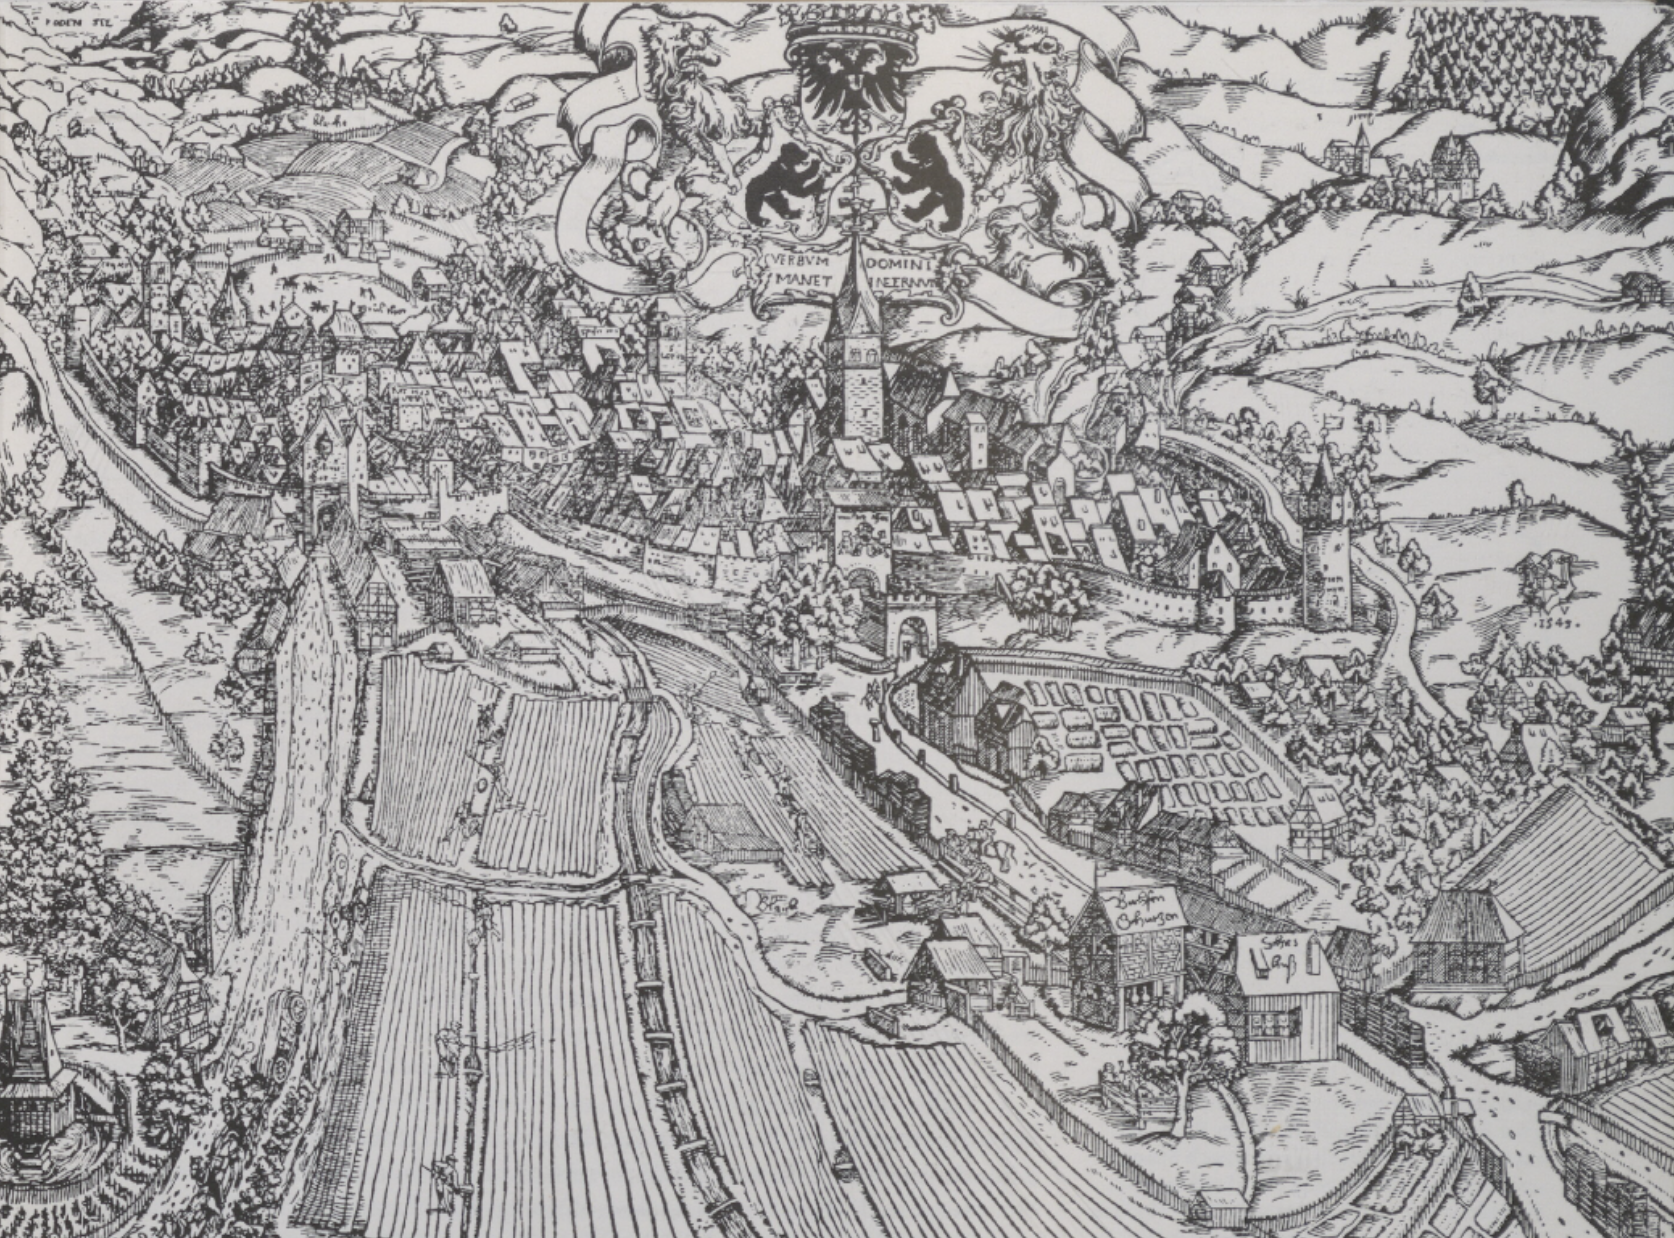
\includegraphics[width=0.8\linewidth]{images/st_gallen_1545.png}
\end{center}

\subsection{Produktion im Verlagssystem}

Die Textilproduktion beruhte überwiegend auf Heimarbeit.

Viele Familien kombinierten textile Tätigkeiten mit Landwirtschaft.
Produziert wurde meist im sogenannten Verlagssystem.

Dabei stellten Kaufleute oder sogenannte Fergger die Verbindung
zwischen Produzenten und Absatzmärkten her.

Sie:

\begin{itemize}
    \item lieferten Rohstoffe
    \item verteilten Aufträge
    \item organisierten den Verkauf
    \item bestimmten häufig die Preise
\end{itemize}

Das Verlagssystem gilt als eine frühe Form der Lohnarbeit
und bereitete spätere industrielle Produktionsformen vor.

Gleichzeitig sorgte das Zunftwesen für Qualitätskontrolle,
schränkte aber technische Neuerungen teilweise ein. 
\subsection{Der Engpass der Garnspinnerei}
\begin{center}
    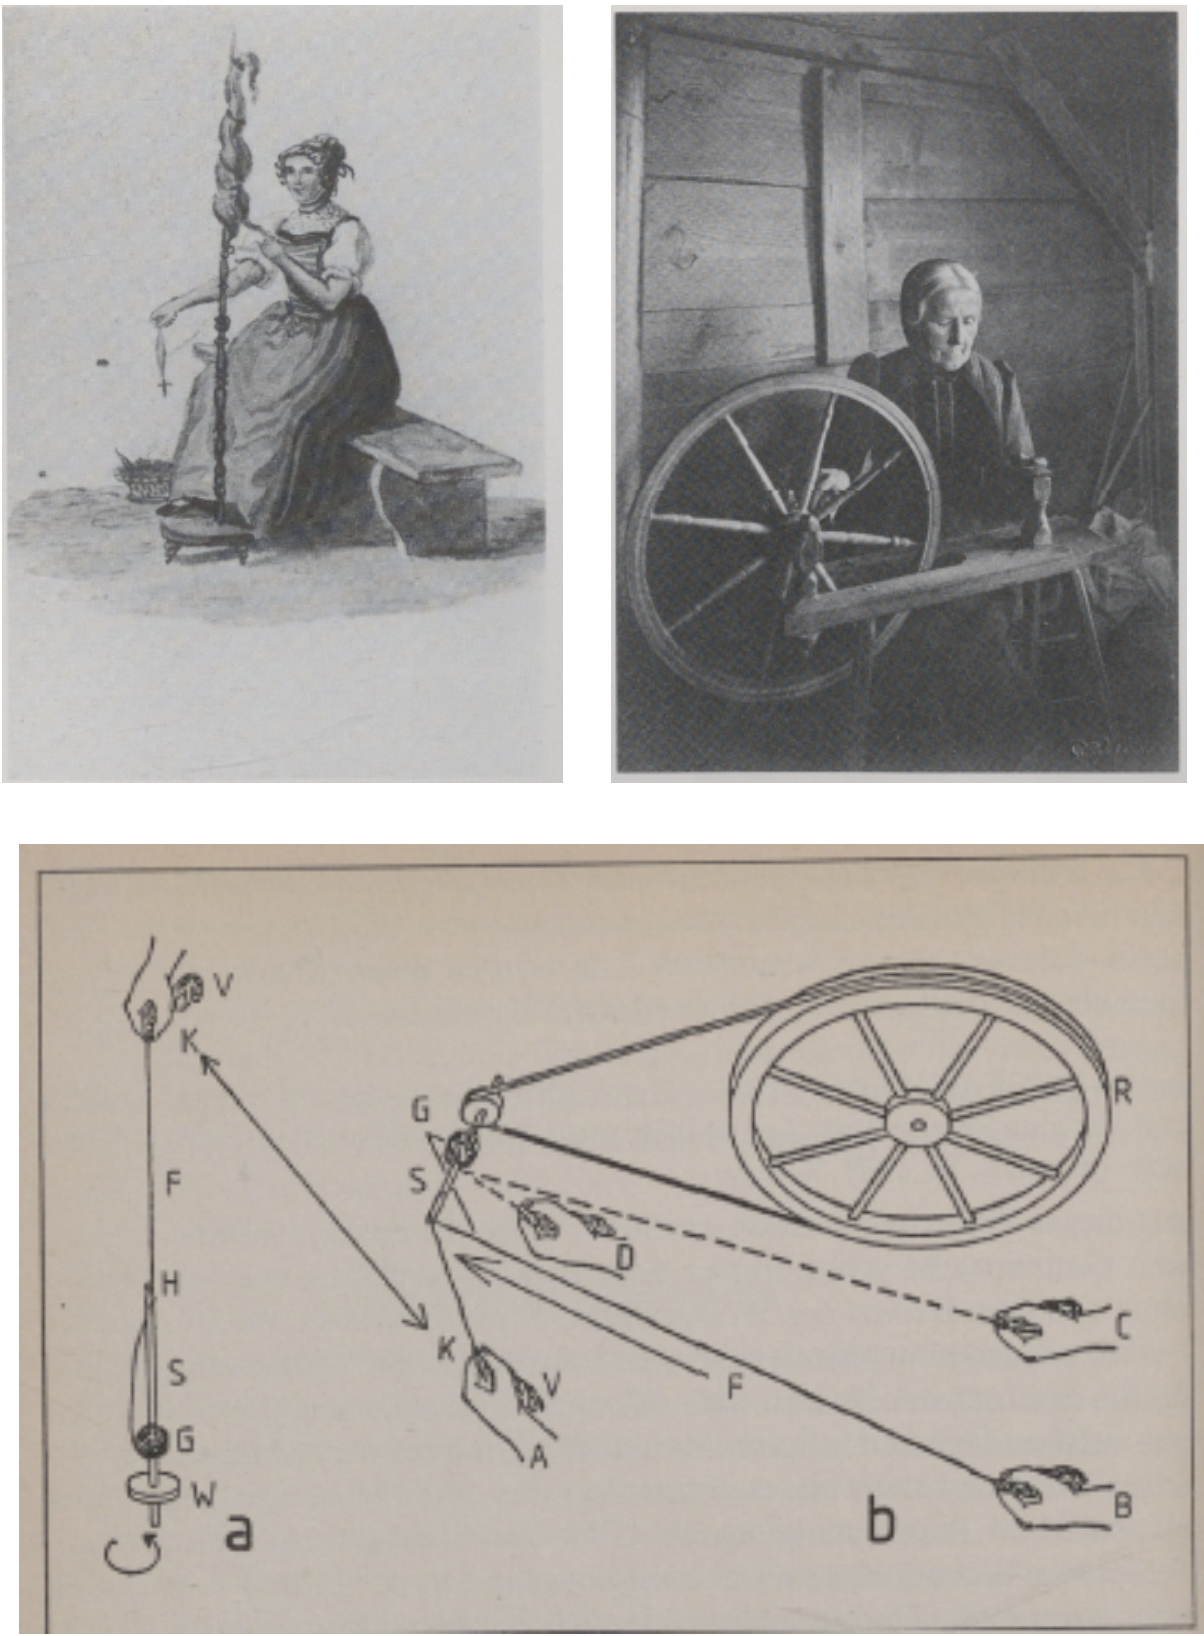
\includegraphics[width=0.7\linewidth]{images/spinning_jenny.png}
\end{center}
Ein zentrales Problem der vorindustriellen Textilproduktion war die Garnherstellung.

Das Spinnen war deutlich arbeitsintensiver als das Weben.

Dadurch entstand ein Produktionsengpass,
der zum Ausgangspunkt wichtiger technischer Innovationen wurde.

Entscheidend waren Entwicklungen aus Grossbritannien:

\begin{itemize}
    \item mechanische Spinnmaschinen wie die Spinning Jenny
    \item die Mule-Spinnmaschine
    \item später mechanische Webstühle
\end{itemize}

Diese Maschinen steigerten die Produktivität erheblich
und ermöglichten eine weitgehende Mechanisierung der Textilherstellung.

Der technische Fortschritt setzte somit zunächst nicht in der Schweiz,
sondern in Grossbritannien ein. 

\subsection{Warum begann die Industrialisierung in Grossbritannien?}

Grossbritannien gilt als Ursprungsland der Industrialisierung.

Von der Mitte des 18. bis zur Mitte des 19. Jahrhunderts
entstanden dort die grundlegenden industriellen Produktionsformen.

Die Mechanisierung breitete sich rasch aus:

\begin{itemize}
    \item Textilindustrie
    \item Maschinenbau
    \item Eisen- und Stahlproduktion
    \item Bergbau
    \item Chemieindustrie
    \item Energieversorgung
    \item Transportwesen
\end{itemize}

Gleichzeitig veränderte sich die Arbeitswelt grundlegend.

Maschinen konnten zunehmend von weniger qualifizierten Arbeitskräften bedient werden,
wodurch Frauen und Kinder verstärkt in die industrielle Produktion eingebunden wurden.

Die Industrialisierung führte ausserdem zu:

\begin{itemize}
    \item Konzentration von Kapital
    \item Entstehung moderner Unternehmen
    \item Ausbau der Kreditwirtschaft
    \item Zentralisierung der Produktion in Fabriken
    \item starkem Städtewachstum
\end{itemize}

Die industrielle Revolution war somit nicht nur eine technische,
sondern auch eine wirtschaftliche und gesellschaftliche Revolution. 

\subsection{Nachholende Industrialisierung in der Schweiz}

Die Schweiz übernahm viele Entwicklungen aus Grossbritannien.

Dieser Prozess wird als nachholende Industrialisierung bezeichnet.

Technologien und Organisationsformen wurden importiert
und an die lokalen Bedingungen angepasst.

Im Verlauf des 19. Jahrhunderts entstanden in der Ostschweiz:

\begin{itemize}
    \item Spinnereien
    \item Webereien
    \item Stickereifabriken
    \item Bleichereien
    \item Veredelungsbetriebe
\end{itemize}

Besonders wichtig war die Einführung des Fabriksystems.

Der Einsatz von Dampfkraft machte Produktionsstandorte
zunehmend unabhängig von Flüssen und Wasserkraft.

Dadurch beschleunigten sich Industrialisierung und Verstädterung erheblich. 

\begin{center}
    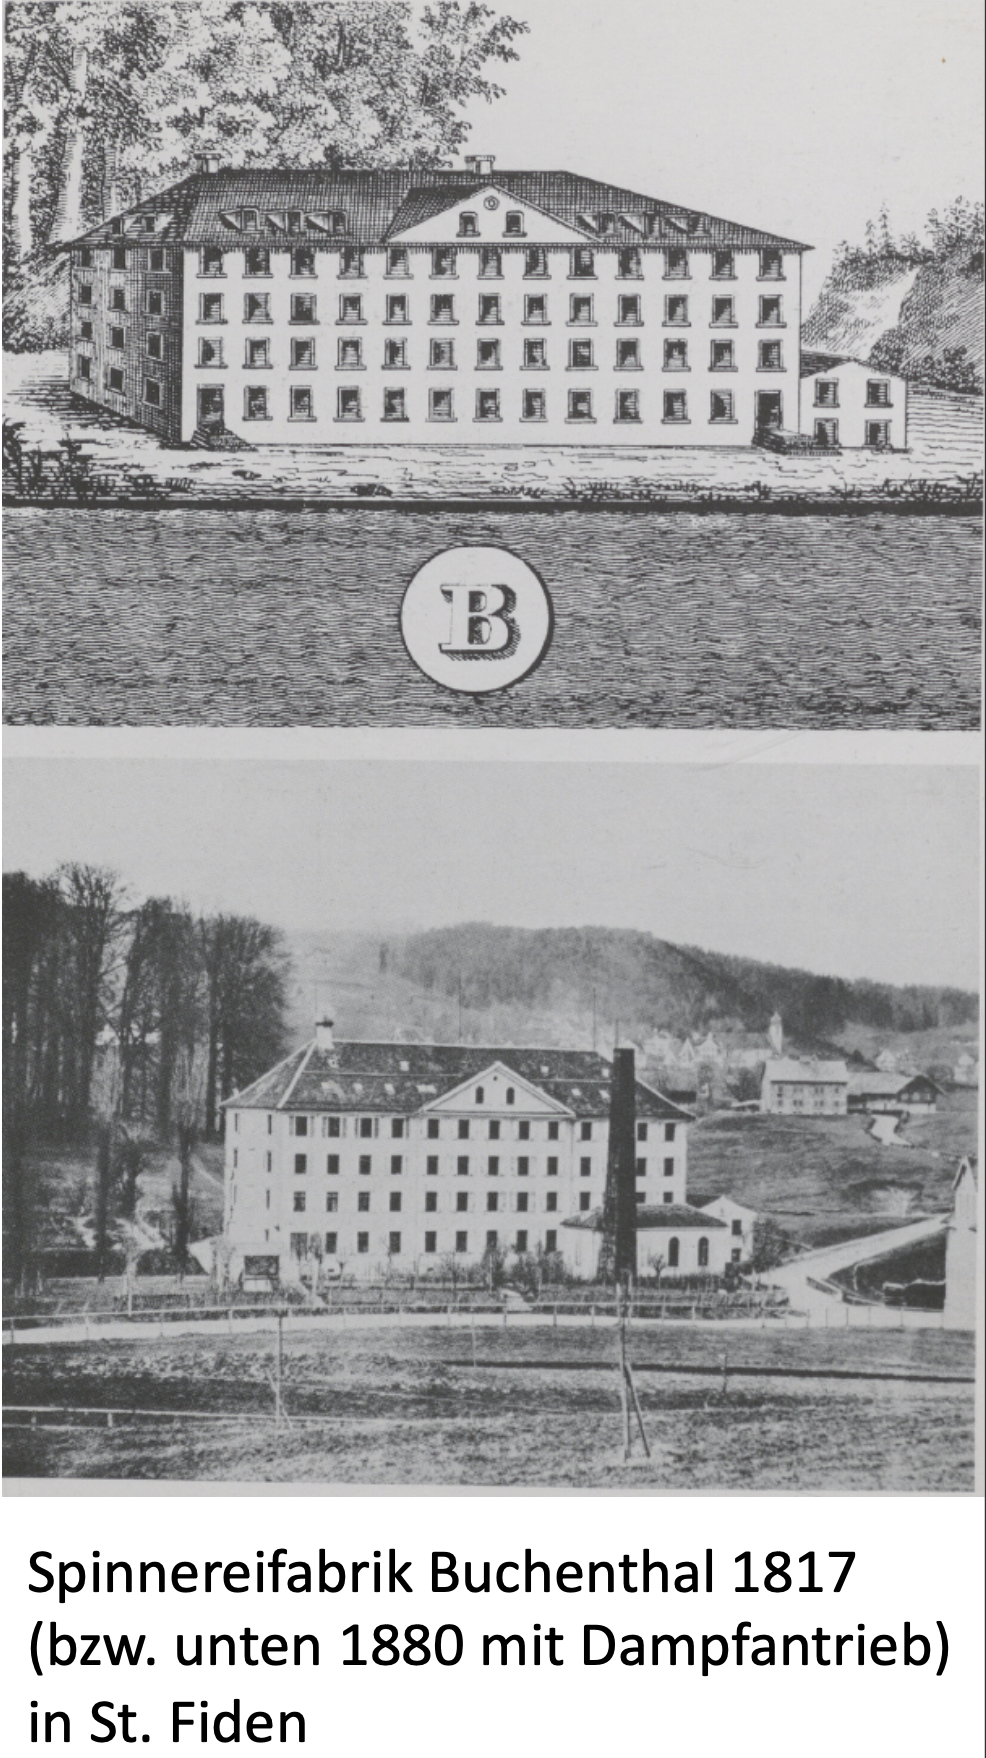
\includegraphics[width=0.8\linewidth]{images/spinnerei_buchental.png}
\end{center}

\subsection{Das Fabriksystem und die soziale Frage}

Mit der Industrialisierung entstanden neue Formen der Arbeit.

Die Fabrik wurde zum zentralen Ort der Produktion.

Damit verbunden waren zahlreiche soziale Probleme:

\begin{itemize}
    \item lange Arbeitszeiten
    \item Kinderarbeit
    \item geringe Arbeitssicherheit
    \item Disziplinierung durch Strafen und Entlassungen
    \item schlechte Arbeitsbedingungen
\end{itemize}

Gleichzeitig entwickelte sich eine neue Arbeiterkultur.

\begin{center}
    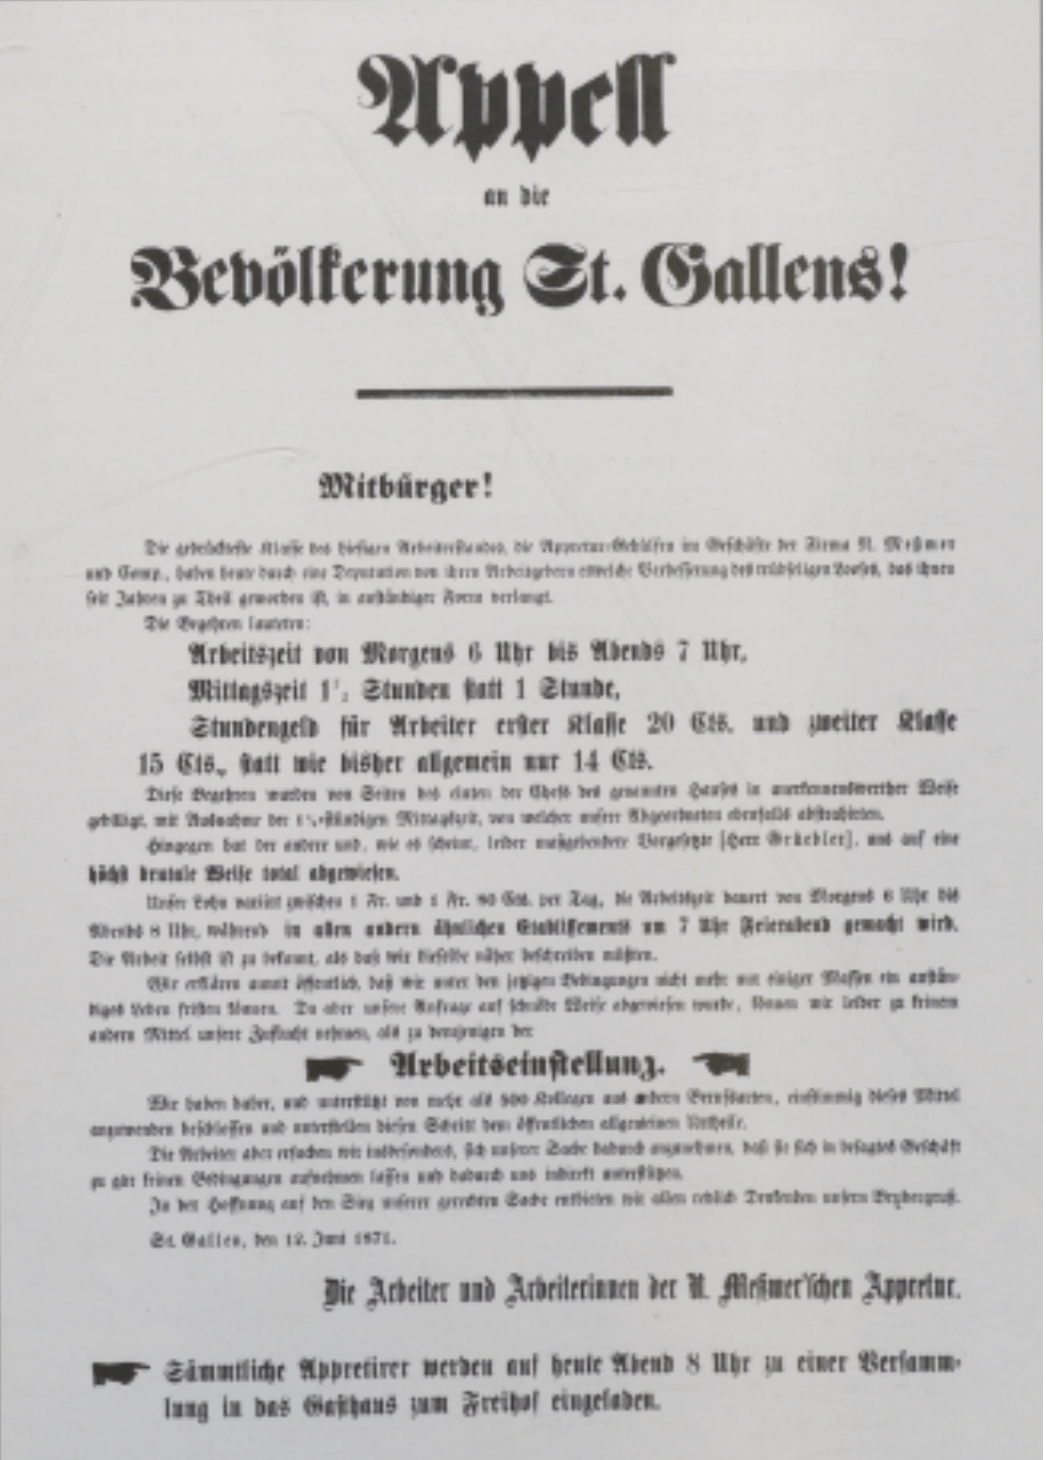
\includegraphics[width=0.6\linewidth]{images/streik_st_gallen_1971.png}
\end{center}

Arbeiterinnen und Arbeiter organisierten sich zunehmend,
bildeten Solidaritätsnetzwerke und führten Streiks durch.

Die Industrialisierung brachte daher sowohl wirtschaftlichen Fortschritt
als auch neue gesellschaftliche Konflikte hervor. 

\subsection{Das Fabrikgesetz von 1877}

Die sozialen Probleme führten schliesslich zu staatlichen Eingriffen.

Mit dem eidgenössischen Fabrikgesetz von 1877
wurden erstmals verbindliche Regeln für Fabriken geschaffen.

Wichtige Bestimmungen waren:

\begin{itemize}
    \item Verbot der Kinderarbeit
    \item Schutz von Gesundheit und Leben der Beschäftigten
    \item Einführung des Elfstundentages
    \item Unfallmeldepflicht
    \item Registrierung der Arbeitnehmer
    \item Regulierung von Disziplinarmassnahmen
    \item Kündigungsschutz
    \item Einführung staatlicher Fabrikinspektoren
\end{itemize}

Das Gesetz markiert einen wichtigen Schritt
vom weitgehend unregulierten Fabrikbetrieb
hin zu staatlich kontrollierten Arbeitsverhältnissen. 

\subsection{Die ostschweizerische Stickereiindustrie}

Im 19. Jahrhundert entwickelte sich die Stickerei
zum bedeutendsten Industriezweig der Ostschweiz.

Gründe dafür waren:

\begin{itemize}
    \item wachsender internationaler Wettbewerb
    \item Spezialisierung auf hochwertige Produkte
    \item hohe Nachfrage nach Stickereiwaren
\end{itemize}

Um 1910 exportierte die Schweiz Stickereien
im Wert von rund 200 Millionen Franken.

Mehr als 60'000 Menschen arbeiteten in den Regionen
St. Gallen, Appenzell und Thurgau in diesem Wirtschaftszweig. 

\subsection{Mechanisierung der Stickerei}

Auch die Stickerei wurde mechanisiert.

Die Einführung von Stickmaschinen ab etwa 1850
steigerte die Produktivität erheblich.

Eine einzelne Maschine konnte die Arbeit
zahlreicher Handstickerinnen ersetzen.

Mit der Schifflistickmaschine ab 1863
wurden zudem körperliche Belastungen reduziert.

Gleichzeitig brachte die Mechanisierung neue Formen der Arbeitsorganisation:

\begin{itemize}
    \item Arbeit nach Maschinentakt
    \item stärkere Arbeitsteilung
    \item höhere Produktionsleistung
\end{itemize}

Anders als in vielen anderen Industrien
blieb jedoch ein grosser Teil der Produktion
weiterhin in Heimarbeit organisiert. 

\begin{center}
    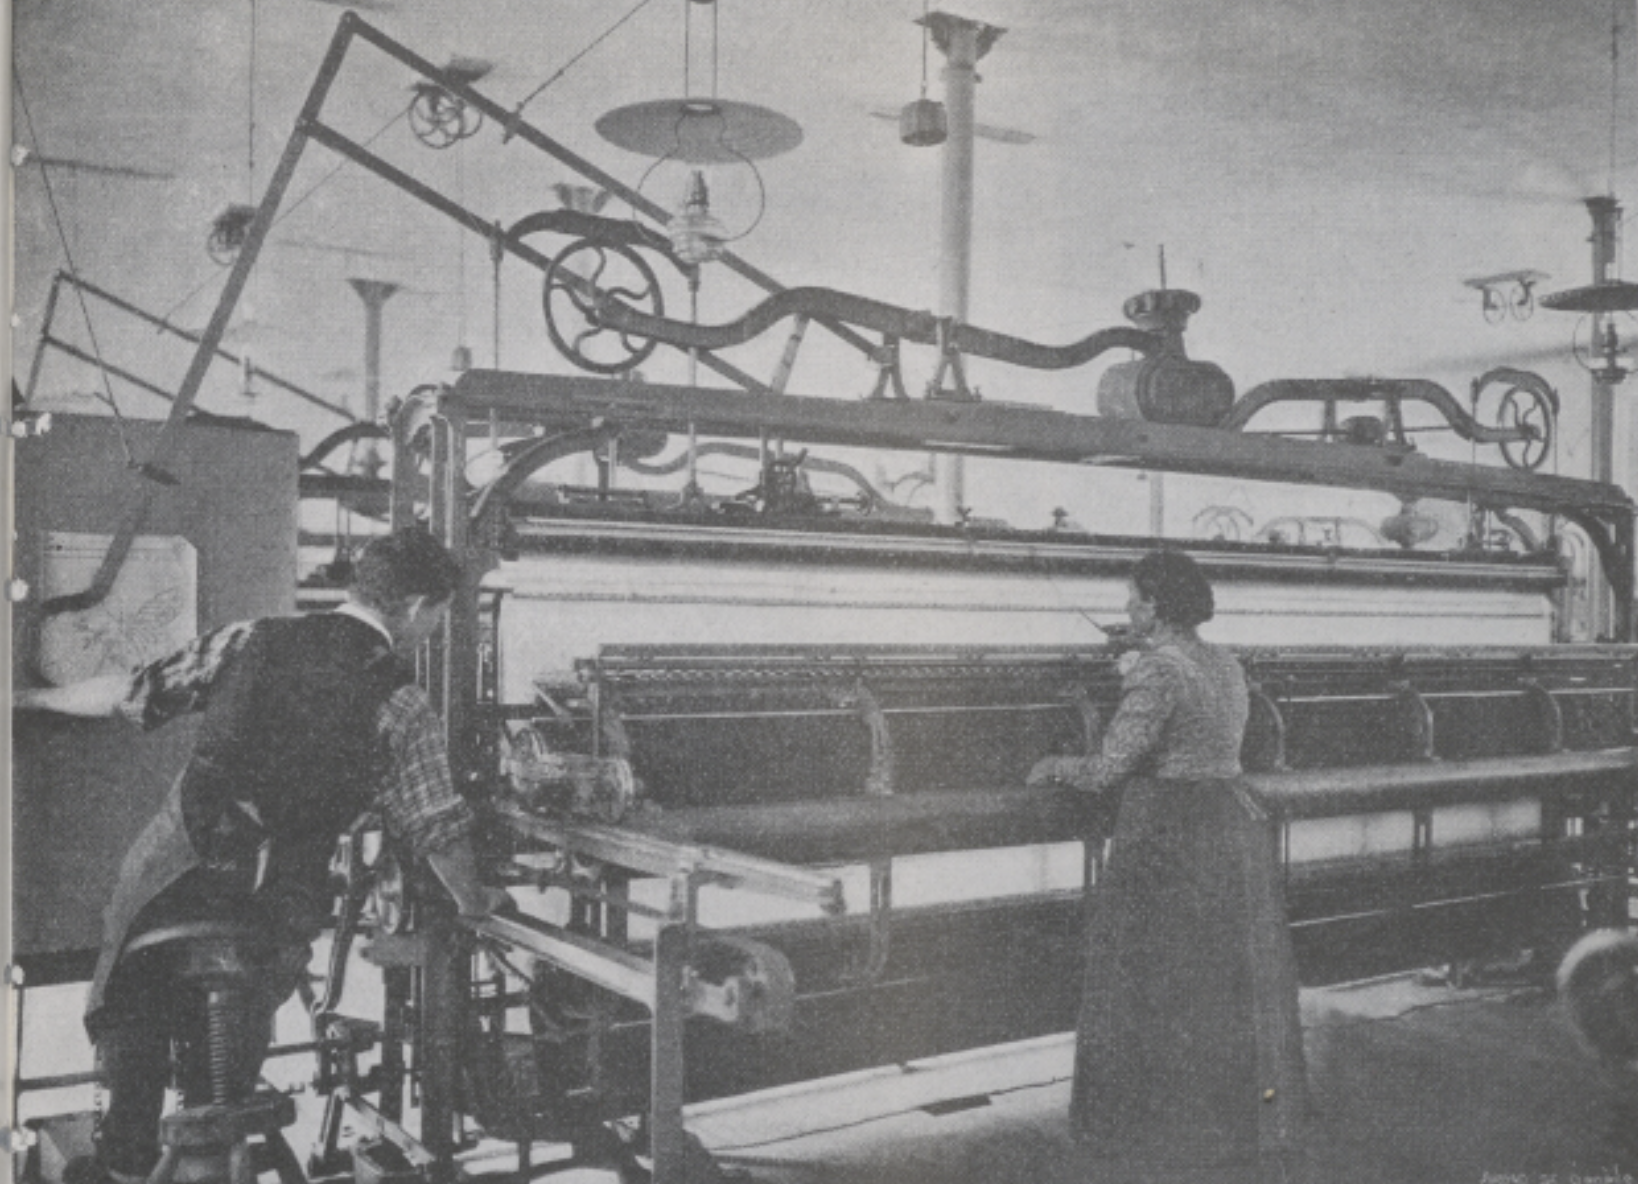
\includegraphics[width=0.8\linewidth]{images/schifflistickmaschine.png}
\end{center}

\subsection{Heimarbeit und das Dilemma der Moderne}

Viele Sticker entschieden sich bewusst gegen die Fabrikarbeit.

Die Heimarbeit versprach:

\begin{itemize}
    \item grössere Selbstständigkeit
    \item flexible Arbeitszeiten
    \item Arbeit im familiären Umfeld
\end{itemize}

Gleichzeitig entstanden neue Abhängigkeiten.

Heimarbeiter mussten:

\begin{itemize}
    \item Maschinen selbst finanzieren
    \item wirtschaftliche Risiken tragen
    \item sich den Vorgaben der Verleger unterordnen
    \item mit starken Marktschwankungen leben
\end{itemize}

Die Industrialisierung führte daher nicht zu einer einfachen Verbesserung der Lebensbedingungen.

Vielmehr entstand ein Spannungsverhältnis zwischen
Fabrikarbeit und scheinbar selbstständiger Heimarbeit.

Dieses Spannungsfeld bezeichnet die Vorlesung als das „Dilemma der Moderne“. 

\begin{center}
    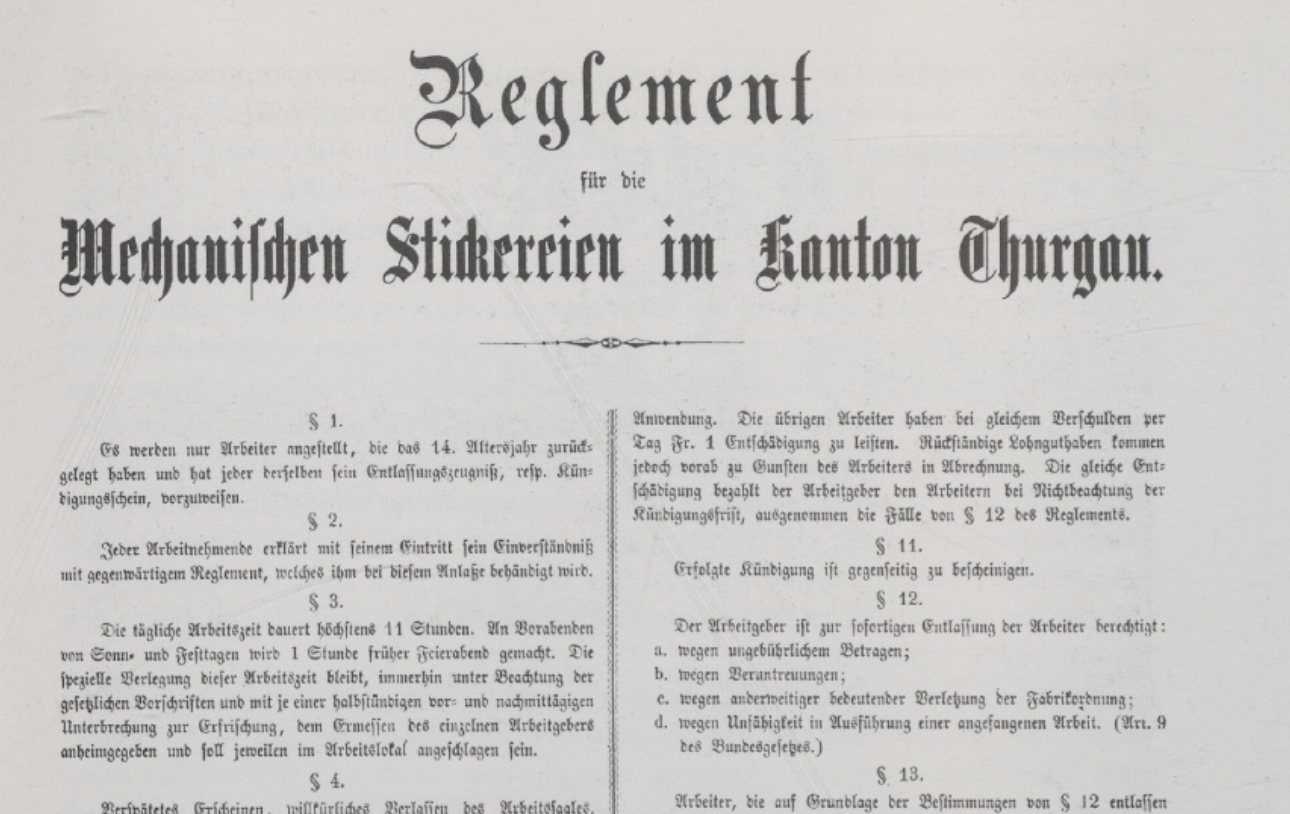
\includegraphics[width=0.6\linewidth]{images/fabrikreglement_stickerei.png}
\end{center}

\subsection{Arbeitsteilung und Geschlechterrollen}

Die Industrialisierung veränderte auch die Geschlechterordnung.

Frauen übernahmen zahlreiche Tätigkeiten
in Textil- und Stickereibetrieben.

Gleichzeitig blieb die Arbeit stark geschlechtsspezifisch organisiert.

Bestimmte Aufgaben wurden Männern,
andere Frauen zugewiesen.

Die industrielle Arbeitsteilung beeinflusste somit nicht nur die Produktion,
sondern auch gesellschaftliche Vorstellungen von Geschlecht und Arbeit. 

\subsection{Das Ende der Stickereiblüte}

Die ostschweizerische Stickerei war stark von Modetrends abhängig.

Nach dem Ersten Weltkrieg veränderten sich Geschmack
und Bekleidungsstile grundlegend.

Die sogenannte Neue Sachlichkeit der 1920er Jahre
bevorzugte schlichte und funktionale Kleidung.

Dadurch sank die Nachfrage nach aufwendigen Stickereien deutlich.

Die einstige Leitindustrie der Ostschweiz verlor ihre wirtschaftliche Bedeutung. 

\subsection{Zentrale Erkenntnisse}

Die Industrialisierung war weit mehr als die Einführung neuer Maschinen.

Sie führte zu tiefgreifenden Veränderungen in Wirtschaft,
Gesellschaft und Alltag.

Die Vorlesung zeigt insbesondere:

\begin{itemize}
    \item den Übergang von der Protoindustrie zum Fabriksystem
    \item die Bedeutung technischer Innovationen für Produktivitätssteigerungen
    \item die Entstehung neuer Arbeitsformen und sozialer Konflikte
    \item die Rolle staatlicher Regulierung
    \item die Wechselwirkungen zwischen Technik, Wirtschaft und Gesellschaft
\end{itemize}

Die zentrale These lautet:

Industrialisierung ist kein rein technischer Prozess.
Sie beschreibt einen umfassenden gesellschaftlichen Wandel,
in dem neue Technologien, wirtschaftliche Interessen und soziale Strukturen
aufeinander einwirken und die moderne Gesellschaft hervorbringen.
        \section{Die Eisenbahn und der Taktfahrplan}

\subsection{Einführung: Verkehr als Grundlage der Moderne}

Die Vorlesung betrachtet die Eisenbahn nicht nur als Transportmittel,
sondern als technische Infrastruktur,
die Wirtschaft, Gesellschaft und Alltag grundlegend veränderte.

Bereits vor der Eisenbahn verbesserten sich Transportmöglichkeiten
durch Strassenbau, Postkutschen, Kanäle und die Dampfschifffahrt.

Mit der Industrialisierung stieg jedoch der Bedarf nach schnelleren,
zuverlässigeren und leistungsfähigeren Verkehrssystemen.

Die Eisenbahn wurde deshalb zu einer der wichtigsten
Fortschrittstechnologien des 19. Jahrhunderts.

Zentrale Leitfragen:

\begin{itemize}
    \item Welche Bedeutung hatte die Eisenbahn für die Industrialisierung?
    \item Wie entwickelte sich das Eisenbahnwesen in der Schweiz?
    \item Weshalb entstand der Taktfahrplan?
    \item Was sagt die Entwicklung der Eisenbahn über gesellschaftlichen Wandel aus?
\end{itemize}

Die Geschichte der Eisenbahn ist daher nicht nur Technikgeschichte,
sondern auch Infrastruktur-, Wirtschafts- und Sozialgeschichte.

\subsection{Die Eisenbahn als Symbol des Fortschritts}

Die moderne Eisenbahn entstand zu Beginn des 19. Jahrhunderts
in Grossbritannien mit der Einführung dampfbetriebener Lokomotiven.

Während Schienenwege bereits seit dem Mittelalter
im Bergbau genutzt wurden,
ermöglichte die Dampflok erstmals einen schnellen
und leistungsfähigen Transport über grössere Distanzen.

In Europa verbanden die ersten Eisenbahnlinien
Industriezentren und Grossstädte.

In Staaten wie den USA spielte die Eisenbahn zusätzlich
eine wichtige Rolle bei der Erschliessung neuer Gebiete.

Die Eisenbahn wurde damit zu einem Symbol
technischen Fortschritts und wirtschaftlicher Modernisierung.

\begin{center}
    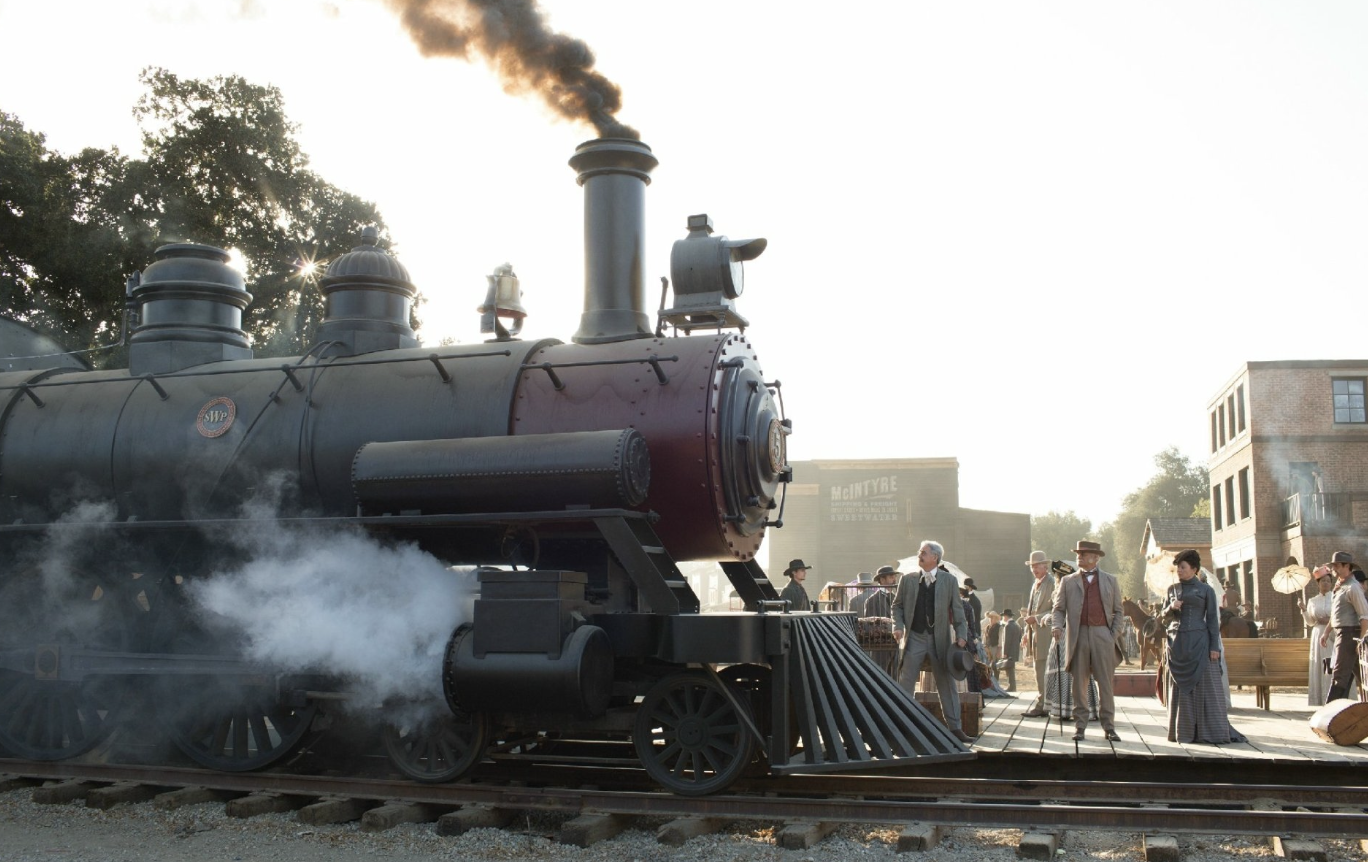
\includegraphics[width=0.8\linewidth]{images/dampflok_fortschritt.png}
\end{center}

\subsection{Die Entwicklung der Eisenbahn in der Schweiz}

Bereits seit den 1820er Jahren entstanden erste Projekte
für ein schweizerisches Eisenbahnnetz.

1847 wurde mit der sogenannten Spanisch-Brödli-Bahn
zwischen Zürich und Baden die erste Eisenbahnlinie eröffnet.

Nach der Gründung des Bundesstaates entwickelte sich
ein stark fragmentiertes Bahnsystem,
in dem private und staatliche Unternehmen miteinander konkurrierten.

Zwischen 1901 und 1909 wurden die grössten Privatbahnen
zu den Schweizerischen Bundesbahnen (SBB) zusammengeführt.

Gleichzeitig entstanden weiterhin regionale Privatbahnen.

Aufgrund fehlender Kohlevorkommen setzte die Schweiz
früh auf die Elektrifizierung des Bahnverkehrs.

Dadurch entwickelte sich die Eisenbahn zu einer zentralen Infrastruktur
des modernen Bundesstaates.

\begin{center}
    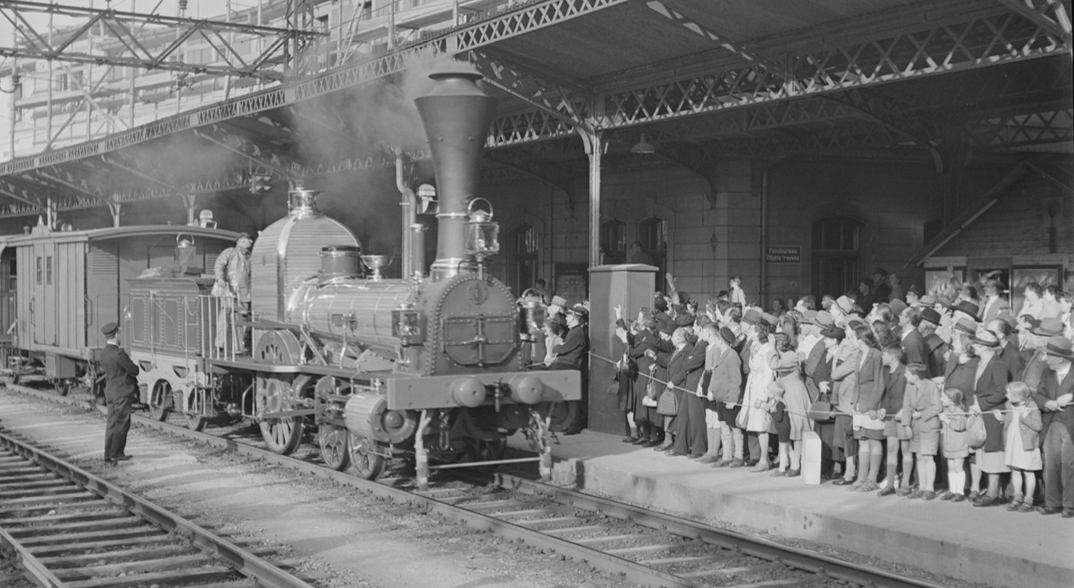
\includegraphics[width=0.8\linewidth]{images/spanisch_broedli_bahn.png}
\end{center}

\subsection{Verkehr, Kommunikation und gesellschaftlicher Wandel}

Die Vorlesung betont,
dass Verkehrssysteme nicht isoliert betrachtet werden können.

Die Entwicklung des Eisenbahnverkehrs
stand in engem Zusammenhang mit neuen Kommunikationsformen.

Dazu gehörten:

\begin{itemize}
    \item die Post
    \item Telegraphennetze
    \item Funktechnik
    \item moderne Sicherungssysteme
\end{itemize}

Transport und Kommunikation entwickelten sich gemeinsam
zu den grundlegenden Infrastrukturen moderner Gesellschaften.

Im Verlauf des 20. Jahrhunderts wandelte sich die Eisenbahn zudem
von einem vorwiegend für Güter genutzten Verkehrsmittel
zu einem Massenverkehrsmittel für die Bevölkerung.

\subsection{Quellenkritik: Das Signalisationssystem der SBB}

Im Zentrum der Quellenanalyse stand das Piktogrammsystem der SBB,
das Ende der 1980er Jahre entwickelt wurde.

Die Quelle besteht aus einer Übersicht der neuen Bahnhofssignalisation
und zeigt standardisierte Symbole für Orientierung,
Dienstleistungen und Verkehrsanschlüsse.

\begin{center}
    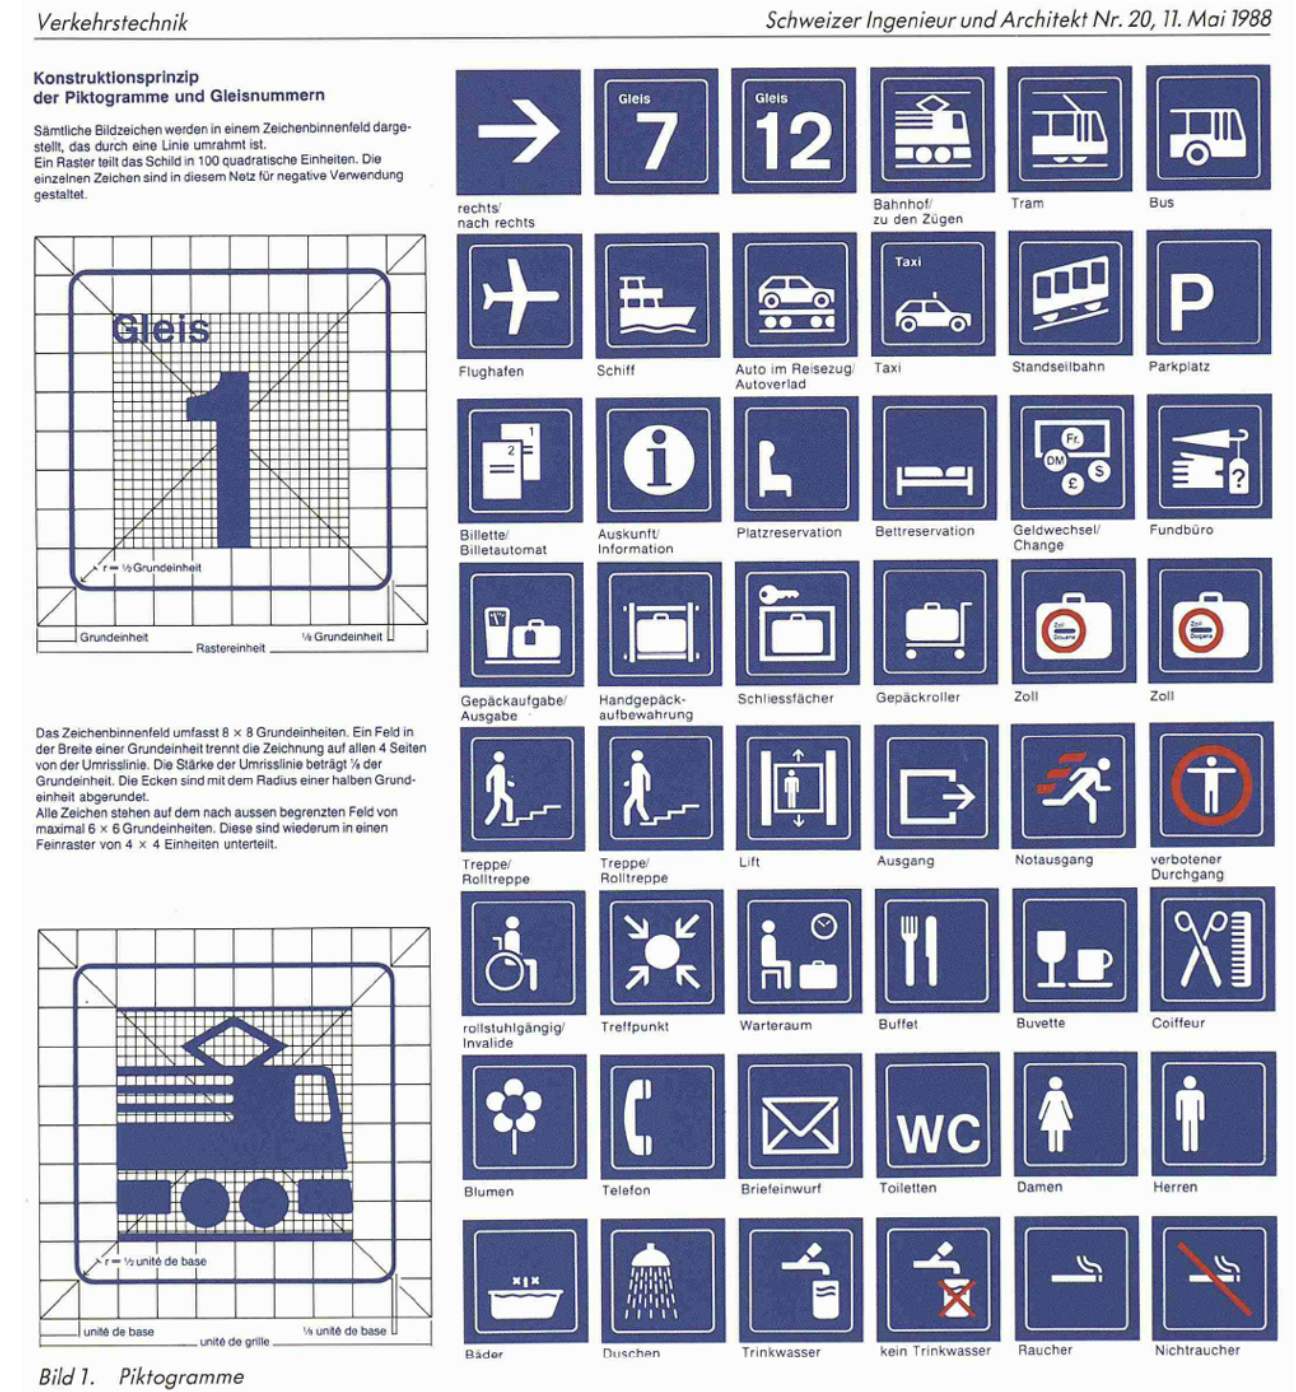
\includegraphics[width=0.9\linewidth]{images/sbb_piktogramme.png}
\end{center}

\paragraph{Äussere Quellenkritik}

Bei der Quelle handelt es sich um eine visuelle Quelle
beziehungsweise um ein technisches Gestaltungskonzept.

Veröffentlicht wurde sie 1988 in der Fachzeitschrift
\textit{Schweizer Ingenieur und Architekt}.

Die Quelle entstand im Umfeld der Schweizerischen Bundesbahnen
und richtet sich sowohl an Fachpersonen
als auch an die breite Öffentlichkeit.

Sie entstand in einer Zeit,
in der die SBB ihre Bahnhöfe modernisierte
und zunehmend auf eine einheitliche Kundenorientierung setzte.

Die Zielgruppe waren nicht mehr nur regelmässige Bahnbenutzer,
sondern auch Gelegenheitsreisende,
Touristen und internationale Fahrgäste.

\paragraph{Innere Quellenkritik}

Die Quelle verfolgt das Ziel,
Orientierung innerhalb komplexer Verkehrsinfrastrukturen
zu vereinfachen.

Die Symbole sollen sprachunabhängig funktionieren
und eine schnelle Informationsaufnahme ermöglichen.

Im Gegensatz zu älteren Beschilderungen
beruht das System auf Standardisierung,
Wiedererkennbarkeit und visueller Klarheit.

Dadurch wird der Bahnhof als übersichtlicher,
effizienter und kundenfreundlicher Raum dargestellt.

Die Gestaltung orientiert sich an internationalen Standards
des Informationsdesigns und der visuellen Kommunikation.

\paragraph{Quelleninterpretation}

Die Quelle zeigt,
dass sich die Rolle der Eisenbahn im Laufe des 20. Jahrhunderts
grundlegend verändert hatte.

Während Bahnhöfe um 1900 vor allem Orte
des Güterverkehrs und des nationalen Reisens waren,
mussten sie in den 1980er Jahren
wachsende Personenströme bewältigen.

Die Signalisation verweist auf neue gesellschaftliche Bedürfnisse:

\begin{itemize}
    \item Mobilität für breite Bevölkerungsschichten
    \item internationale Reisemöglichkeiten
    \item Orientierung unabhängig von Sprache
    \item schnelle Informationsverarbeitung
    \item kundenorientierte Dienstleistungen
\end{itemize}

Die SBB verfolgte mit der neuen Signalisation
das Ziel, Bahnhöfe effizienter nutzbar zu machen
und die Attraktivität des öffentlichen Verkehrs zu steigern.

Die Quelle zeigt somit,
dass technische Infrastruktur zunehmend
auf Benutzerfreundlichkeit und Service ausgerichtet wurde.

Sie kann daher als Ausdruck einer Gesellschaft verstanden werden,
die Mobilität als selbstverständlichen Bestandteil des Alltags betrachtet.

\subsection{Der Taktfahrplan als organisatorische Innovation}

Ein entscheidender Entwicklungsschritt erfolgte 1982
mit der Einführung des schweizweiten Taktfahrplans.

Das Konzept wurde von Samuel Stähli,
Hans Meiner und Jean-Pierre Berthouzoz entwickelt.

Vorbilder fanden sich in den Niederlanden,
bei städtischen Verkehrsbetrieben
und auf einzelnen Bahnstrecken der Schweiz.

Ziel war es,
nicht primär neue Strecken zu bauen,
sondern bestehende Infrastruktur effizienter zu nutzen.

Der Taktfahrplan stellt damit eine organisatorische Innovation dar,
bei der Planung und Koordination wichtiger werden
als technische Neuerungen an Fahrzeugen oder Gleisen.

\subsection{Der „Spinner Club“ und neue Denkweisen}

Die Entwicklung des Taktfahrplans begann bereits Ende der 1960er Jahre.

Eine informelle Arbeitsgruppe innerhalb der SBB,
später als „Spinner Club“ bezeichnet,
arbeitete über Jahre an neuen Konzepten.

Die Gruppe versuchte,
innerhalb einer grossen und stark hierarchischen Organisation
alternative Lösungen für die Zukunft des Bahnverkehrs zu entwickeln.

Die Geschichte des Taktfahrplans zeigt damit,
dass Innovation nicht nur durch neue Technologien entsteht,
sondern auch durch neue organisatorische Ideen.

\begin{center}
    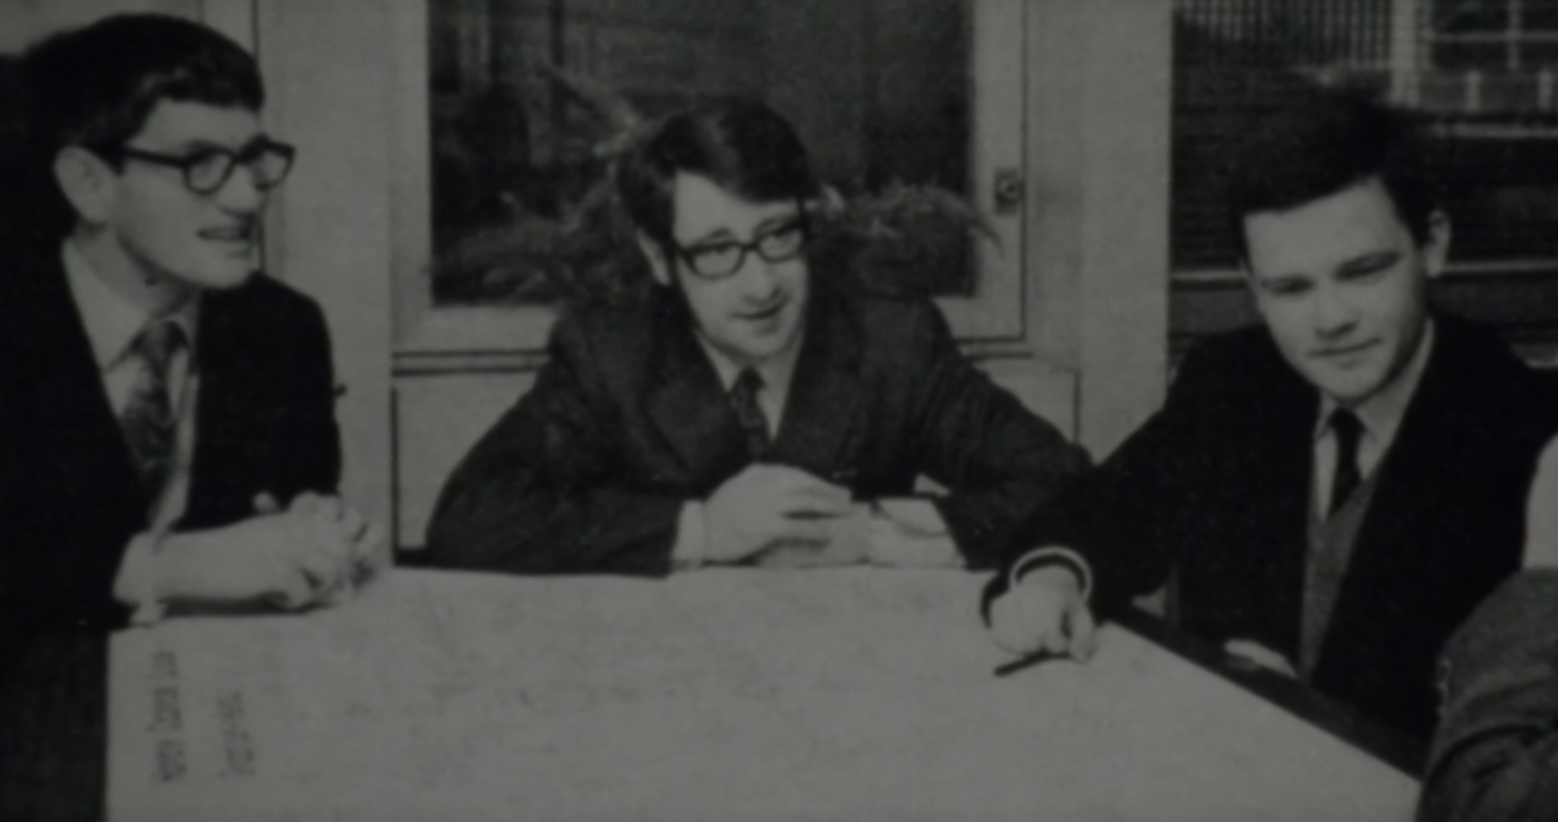
\includegraphics[width=0.7\linewidth]{images/spinner_club.png}
\end{center}

\subsection{Vom Verkehrsmittel zum Mobilitätsangebot}

Mit dem Taktfahrplan veränderte sich die Logik des Bahnbetriebs.

Statt sich ausschliesslich an bestehender Nachfrage zu orientieren,
schufen die SBB ein regelmässiges und leicht verständliches Angebot.

Ziele waren:

\begin{itemize}
    \item Effizienzsteigerung
    \item bessere Anschlüsse
    \item höhere Attraktivität des Bahnverkehrs
    \item Konkurrenzfähigkeit gegenüber dem Auto
\end{itemize}

Die Eisenbahn entwickelte sich dadurch
von einem reinen Transportmittel
zu einem umfassenden Mobilitätssystem.

\begin{center}
    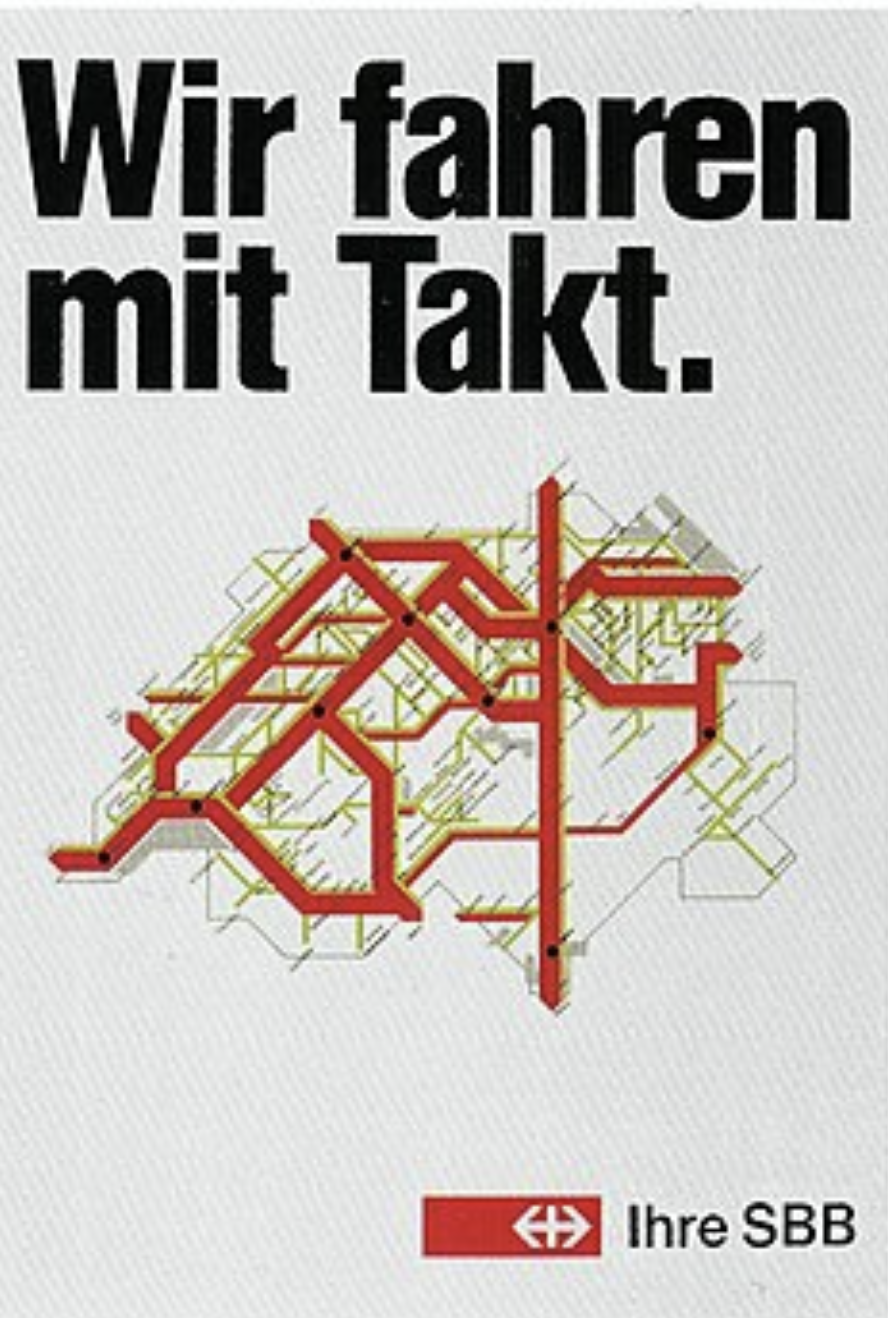
\includegraphics[width=0.55\linewidth]{images/wir_fahren_mit_takt.png}
\end{center}

\subsection{Zentrale Erkenntnisse}

Die Geschichte der Eisenbahn zeigt,
dass technische Innovationen stets mit organisatorischen
und gesellschaftlichen Veränderungen verbunden sind.

Die Vorlesung verdeutlicht insbesondere:

\begin{itemize}
    \item die Rolle der Eisenbahn für die Industrialisierung
    \item die Entstehung nationaler Infrastrukturen
    \item die Bedeutung von Kommunikation und Verkehr
    \item den Wandel zu kundenorientierten Verkehrssystemen
    \item die Bedeutung organisatorischer Innovationen wie des Taktfahrplans
\end{itemize}

Die zentrale These lautet:

Die Entwicklung der Eisenbahn ist nicht nur eine Geschichte
technischer Maschinen und Fahrzeuge.
Sie ist zugleich die Geschichte einer Gesellschaft,
die Mobilität, Orientierung und Vernetzung
zu zentralen Bestandteilen ihres Alltags macht.
        \section{(Auto-)Mobile Society}

\subsection{Einführung: Vom Industrie- zum Konsumzeitalter}

Die Vorlesung untersucht die gesellschaftlichen Veränderungen,
die sich in der zweiten Hälfte des 20. Jahrhunderts vollziehen.

Im Mittelpunkt steht dabei das Automobil,
das nicht nur ein technisches Artefakt,
sondern auch ein Symbol moderner Mobilität,
individueller Freiheit und gesellschaftlichen Wandels darstellt.

Die Vorlesung knüpft an die vorherige Sitzung über Eisenbahn und Taktfahrplan an.

Während dort die Entwicklung öffentlicher Verkehrsinfrastrukturen im Zentrum stand,
rückt nun der Individualverkehr in den Fokus.

Zentrale Leitfragen:

\begin{itemize}
    \item Wie wurde das Automobil zum Massenkonsumgut?
    \item Welche gesellschaftlichen Veränderungen ermöglichte die Massenmotorisierung?
    \item Wie hängen Mobilität, Konsum und industrielle Produktion zusammen?
    \item Welche Formen von Kontrolle und Disziplinierung stehen hinter individueller Freiheit?
\end{itemize}

Die Geschichte des Automobils ist daher nicht nur Technikgeschichte,
sondern auch Konsum-, Sozial- und Kulturgeschichte.

\subsection{Massenmotorisierung und individuelle Freiheit}

Die breite Verfügbarkeit des Automobils setzte in den USA bereits
vor dem Zweiten Weltkrieg ein.

In Europa entwickelte sich die Massenmotorisierung
vor allem nach 1945.

Das Auto wurde zum Symbol persönlicher Freiheit.

Neue Möglichkeiten entstanden für:

\begin{itemize}
    \item Freizeit und Tourismus
    \item Ausflüge und Reisen
    \item räumliche Unabhängigkeit
    \item individuelle Lebensgestaltung
\end{itemize}

Mobilität wurde zunehmend als selbstverständlicher Bestandteil
des modernen Lebens verstanden.

\begin{center}
    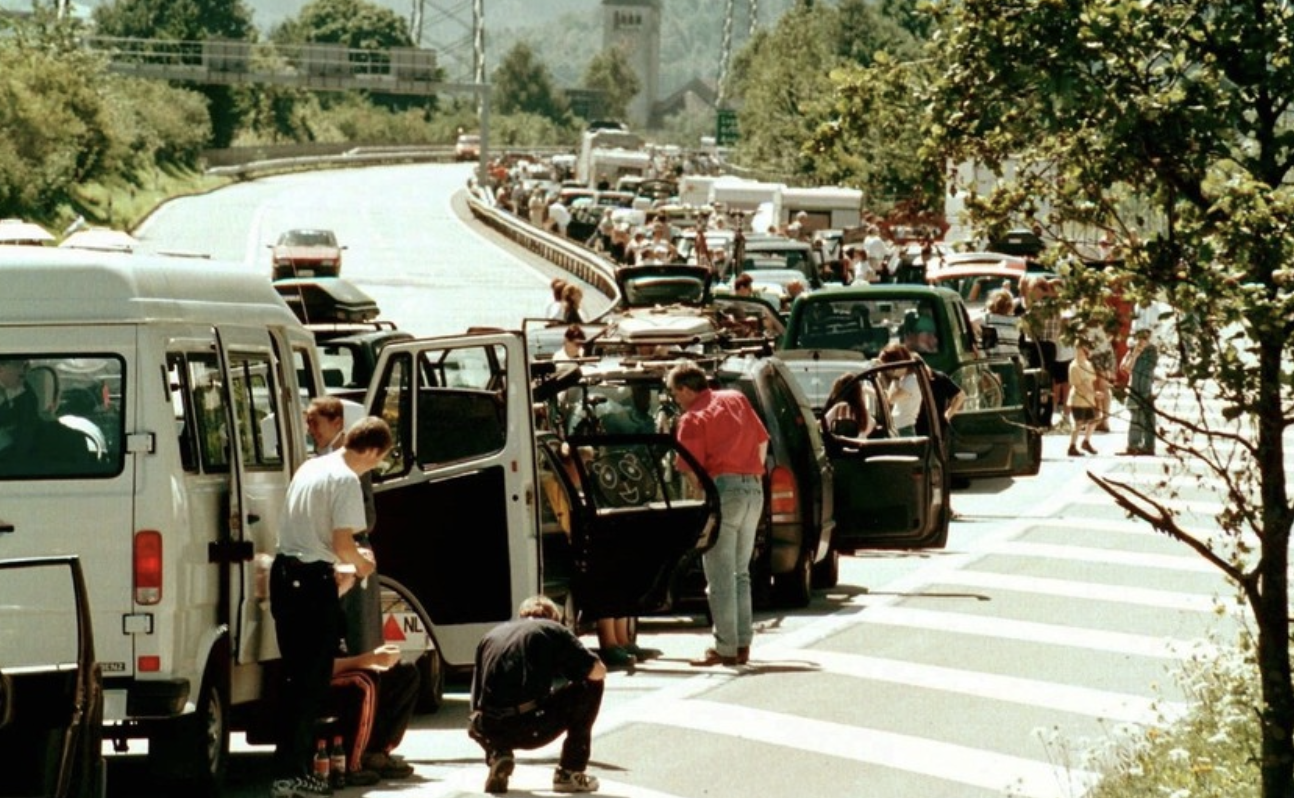
\includegraphics[width=0.75\linewidth]{images/gotthard_stau.png}
\end{center}

\subsection{Automobilisierung und neue Lebensformen}

Die Ausbreitung des Automobils veränderte nicht nur den Verkehr,
sondern auch die Siedlungsstrukturen.

Mit der zunehmenden Verbreitung von Autos entstanden Vororte
und neue Wohnformen ausserhalb der Stadtzentren.

Kennzeichnend waren:

\begin{itemize}
    \item Suburbanisierung
    \item Ausbau des Strassennetzes
    \item räumliche Trennung von Wohnen und Arbeiten
    \item Orientierung am bürgerlichen Lebensstil
\end{itemize}

Die moderne Mobilität veränderte dadurch ganze Landschaften
und prägte den Alltag breiter Bevölkerungsschichten.

\begin{center}
    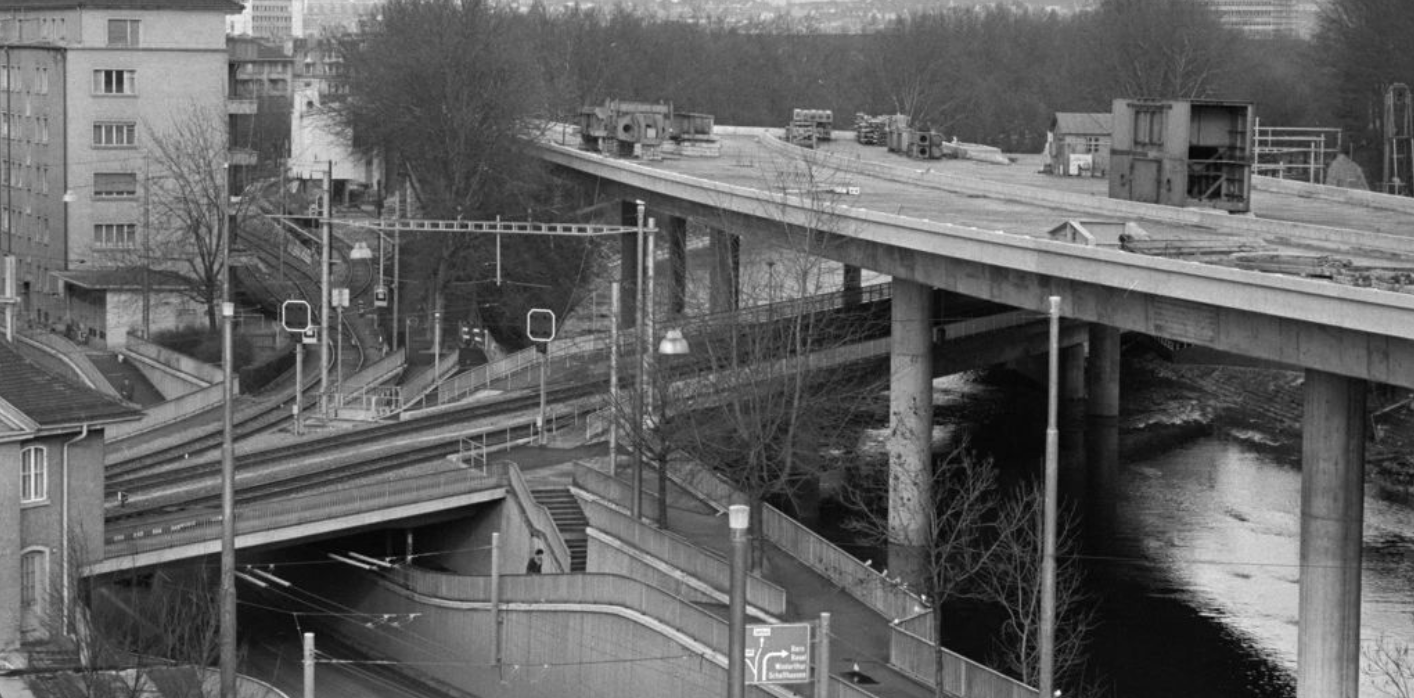
\includegraphics[width=0.8\linewidth]{images/suburbia_autobahn.png}
\end{center}

\subsection{Die frühen Konflikte des Automobils}

Die Einführung des Automobils verlief keineswegs konfliktfrei.

Zu Beginn des 20. Jahrhunderts konkurrierte das Auto
mit etablierten Verkehrsmitteln wie dem Fahrrad,
dem Fussverkehr und dem Pferdeverkehr.

Kritisiert wurden insbesondere:

\begin{itemize}
    \item Lärm
    \item Staubentwicklung
    \item Unfallgefahren
    \item Eingriffe in bestehende Verkehrsordnungen
\end{itemize}

Die Geschichte des Automobils zeigt,
dass technische Innovationen häufig gesellschaftliche Aushandlungsprozesse auslösen.

\begin{center}
    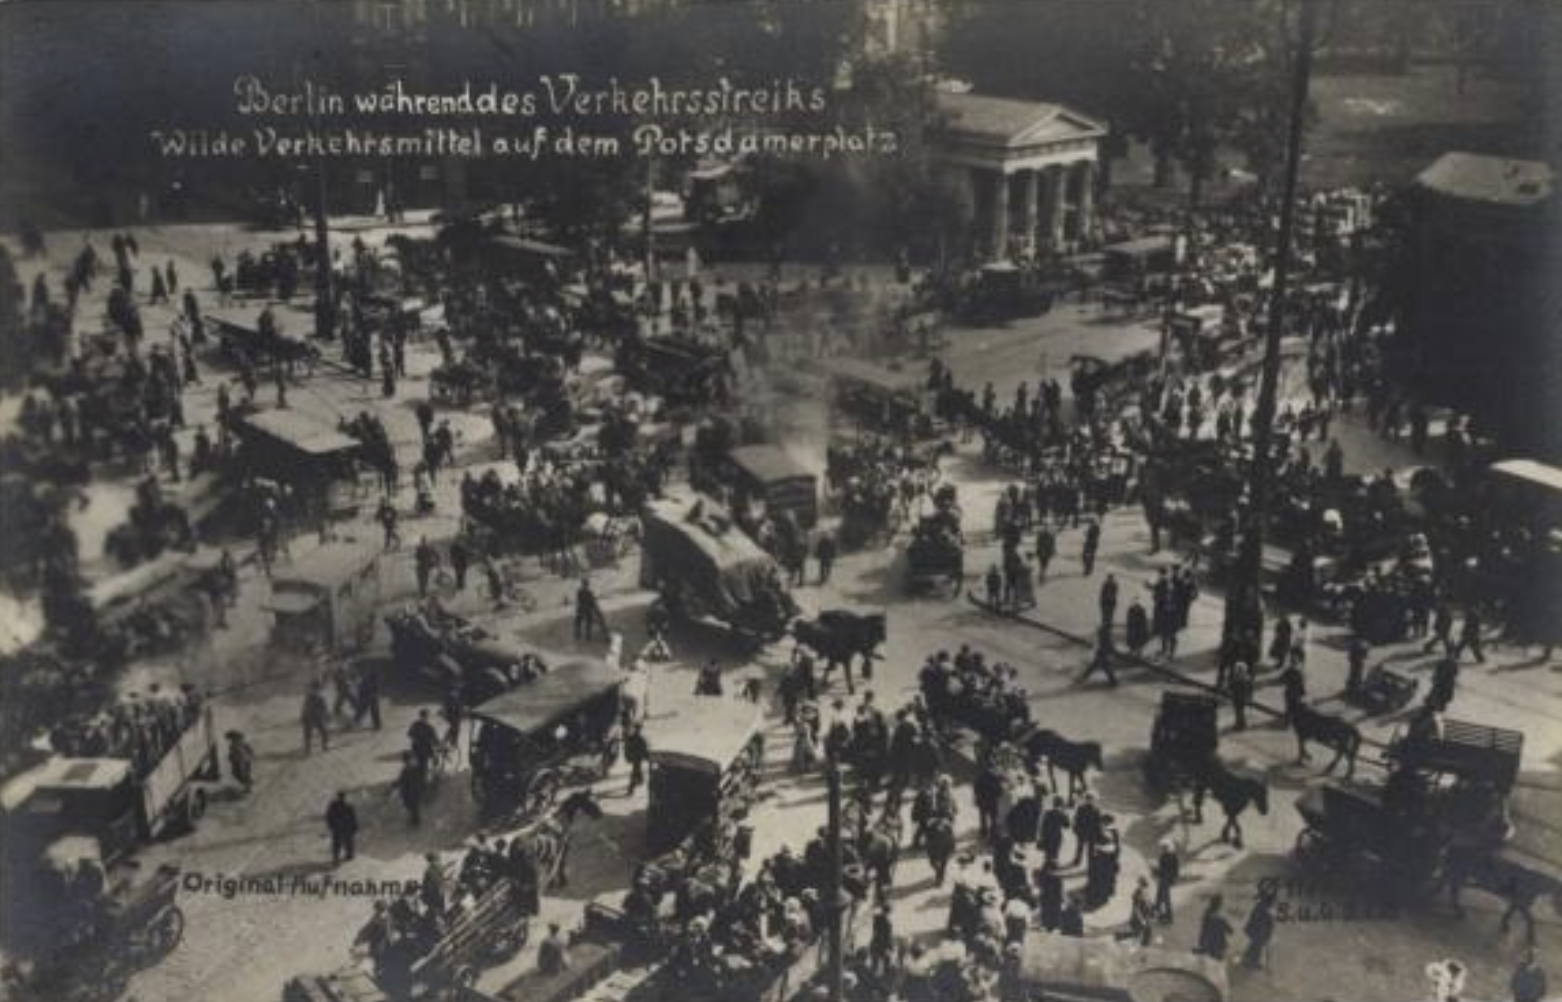
\includegraphics[width=0.75\linewidth]{images/potsdamerplatz_1921.png}
\end{center}

\subsection{Das Auto als Symbol von Geschwindigkeit und Individualismus}

Schon früh wurde das Automobil nicht nur als Transportmittel,
sondern auch als Freizeit- und Sportgerät inszeniert.

Autorennen erfüllten mehrere Funktionen:

\begin{itemize}
    \item Erprobung neuer Technologien
    \item Werbung für Hersteller
    \item Inszenierung technischer Leistungsfähigkeit
    \item Vermarktung von Geschwindigkeit und Freiheit
\end{itemize}

Dadurch entstand das bis heute wirksame Bild des Autos
als Ausdruck von Individualität und persönlicher Unabhängigkeit.

\begin{center}
    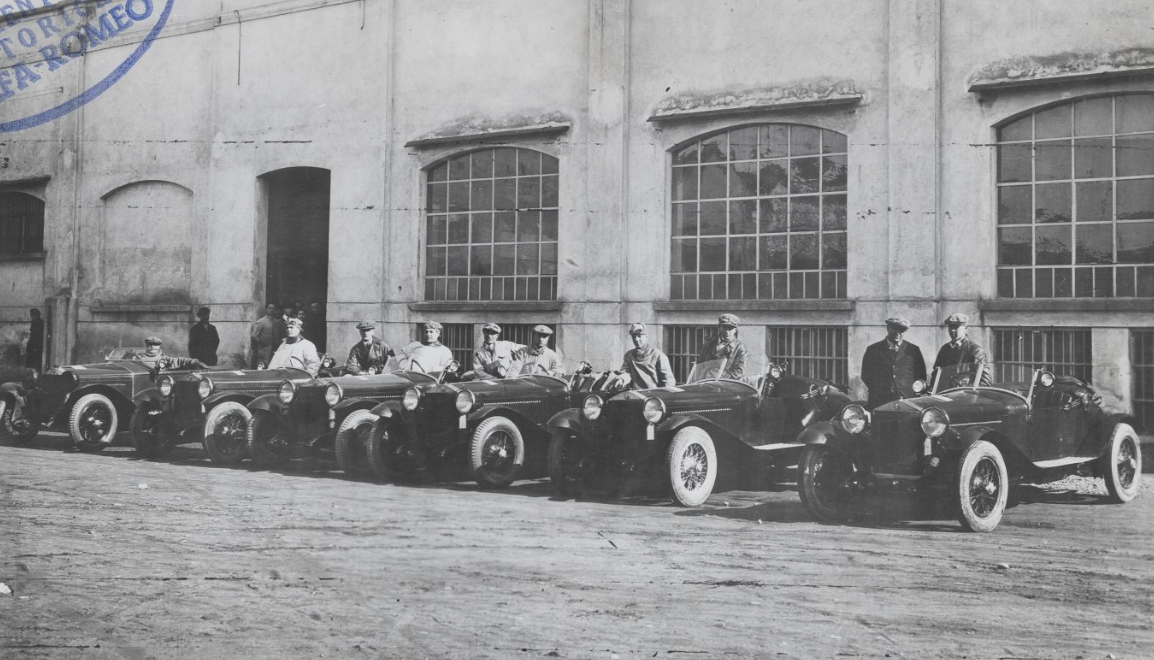
\includegraphics[width=0.75\linewidth]{images/autorennen_fruehes_20jh.png}
\end{center}

\subsection{Vom Industrieprodukt zum Konsumgut}

Die Vorlesung stellt die Frage,
wie das Automobil vom Luxusobjekt zum Massenprodukt werden konnte.

Der Schlüssel liegt in der Entwicklung neuer Produktionsformen.

Technische Innovationen allein genügten nicht.

Entscheidend waren neue Organisationsformen der Arbeit,
die eine kostengünstige Massenproduktion ermöglichten.

\subsection{Taylorismus und wissenschaftliche Arbeitsorganisation}

Ende des 19. Jahrhunderts entwickelte Frederick Winslow Taylor
das Konzept des Scientific Management.

Ziel war die wissenschaftliche Optimierung industrieller Arbeit.

Kennzeichnend waren:

\begin{itemize}
    \item Zerlegung komplexer Tätigkeiten in Einzelschritte
    \item Standardisierung von Arbeitsabläufen
    \item Zeitmessung mit Stoppuhren
    \item Trennung von Planung und Ausführung
    \item Kontrolle der Arbeitsleistung
\end{itemize}

Der Taylorismus bildete eine wichtige Grundlage
für die spätere Massenproduktion.

\subsection{Die Bewegungsstudien der Gilbreths}

Frank und Lillian Gilbreth erweiterten den Taylorismus
durch die systematische Analyse menschlicher Bewegungen.

Mithilfe von Fotografie und sogenannten Chronocyclegraphs
wurden einzelne Handgriffe sichtbar gemacht.

Ziel war die Reduktion unnötiger Bewegungen
und die weitere Steigerung der Effizienz.

Der menschliche Körper wurde damit selbst
zum Gegenstand technischer Optimierung.

\begin{center}
    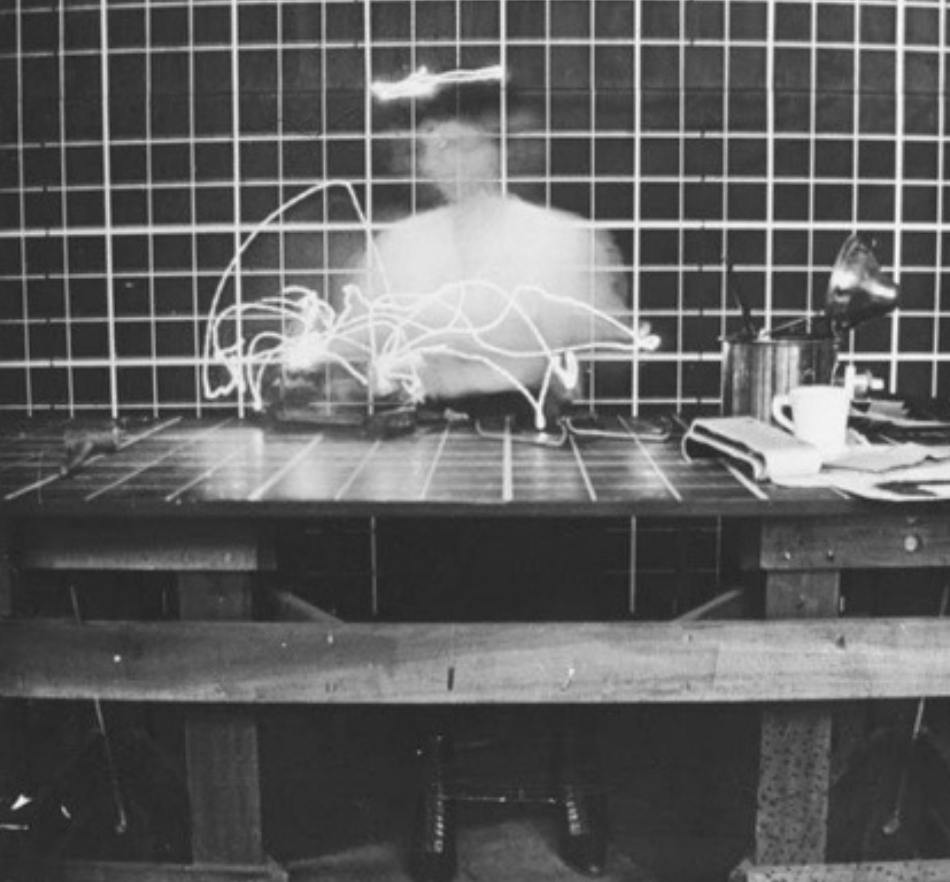
\includegraphics[width=0.7\linewidth]{images/gilbreth_studie.png}
\end{center}

\subsection{Fordismus und Fliessbandproduktion}

Mit Henry Ford erreichte die Rationalisierung industrieller Arbeit
eine neue Stufe.

Ab 1913 wurde die Automobilproduktion
durch das Fliessband grundlegend verändert.

Merkmale des Fordismus:

\begin{itemize}
    \item kontinuierliche Massenfertigung
    \item standardisierte Arbeitsschritte
    \item hohe Produktionszahlen
    \item sinkende Produktionskosten
    \item Taktung der Arbeit durch Maschinen
\end{itemize}

Die Geschwindigkeit der Maschinen bestimmte nun den Arbeitsrhythmus der Beschäftigten.

Dadurch wurde das Automobil erstmals für breite Bevölkerungsschichten erschwinglich.

\begin{center}
    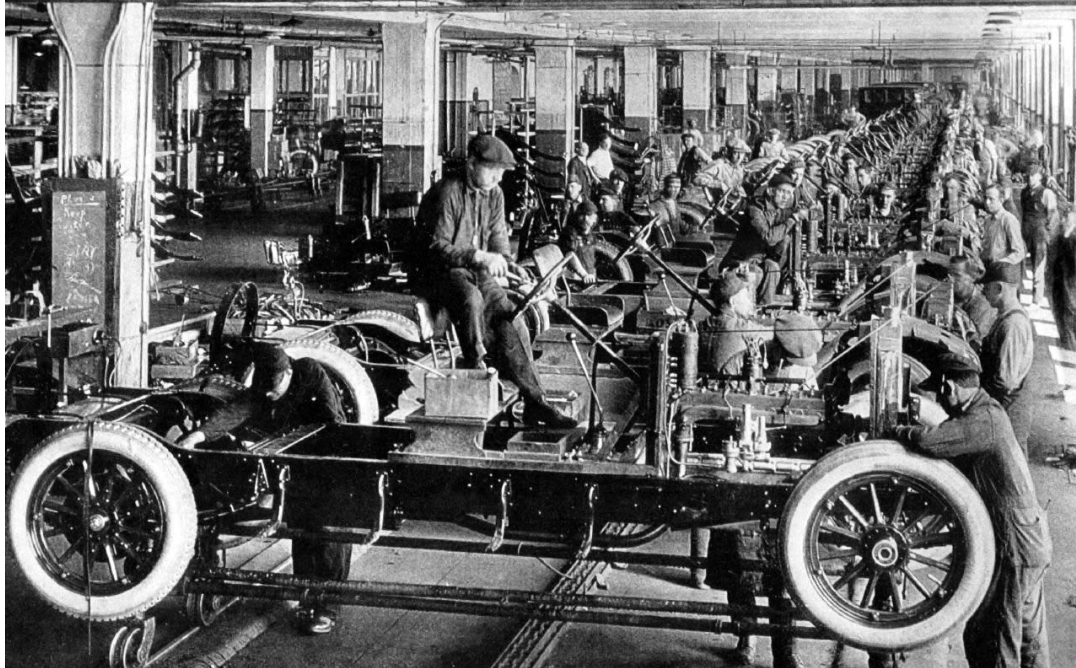
\includegraphics[width=0.8\linewidth]{images/ford_fliessband.png}
\end{center}

\subsection{Globale Rohstoffe und Fordlândia}

Die Automobilproduktion war auf globale Rohstoffketten angewiesen.

Besonders wichtig war Kautschuk für die Herstellung von Reifen.

Der weltweite Kautschukhandel beruhte vielfach
auf kolonialen Herrschaftsverhältnissen und Ausbeutung.

Henry Ford versuchte deshalb,
mit der brasilianischen Siedlung Fordlândia
eine eigene Kautschukproduktion aufzubauen.

Das Projekt scheiterte jedoch.

Die Ursachen lagen in:

\begin{itemize}
    \item fehlender Kenntnis lokaler Bedingungen
    \item ökologischen Problemen
    \item Widerstand der lokalen Bevölkerung
\end{itemize}

Die Geschichte von Fordlândia verdeutlicht,
dass technische und wirtschaftliche Modelle
nicht beliebig auf andere Gesellschaften übertragen werden können.

\begin{center}
    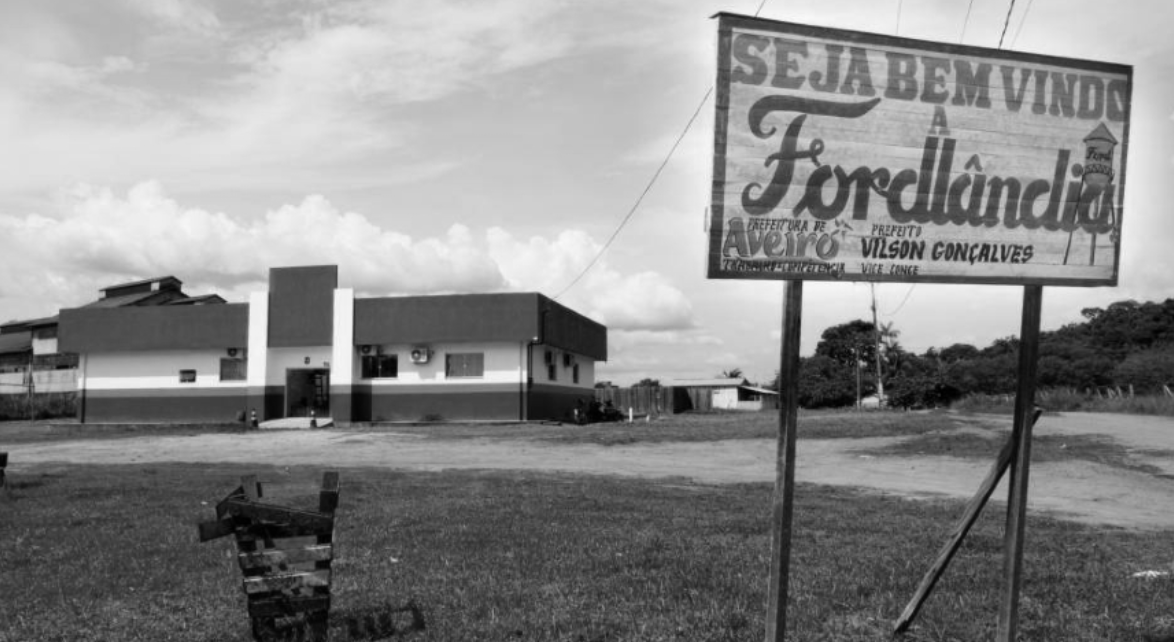
\includegraphics[width=0.75\linewidth]{images/fordlandia.png}
\end{center}

\subsection{Produzenten und Konsumenten}

Ford veränderte nicht nur die Produktion,
sondern auch die Beziehung zwischen Unternehmen und Beschäftigten.

1914 führte Ford vergleichsweise hohe Löhne
und kürzere Arbeitszeiten ein.

Ziel war es,

\begin{itemize}
    \item die Fluktuation zu reduzieren
    \item die Produktivität zu steigern
    \item Arbeiter zu Konsumenten zu machen
\end{itemize}

Gleichzeitig kontrollierte das Unternehmen
über das sogenannte Sociological Department
das Privatleben seiner Beschäftigten.

Die Entstehung der Konsumgesellschaft war damit eng
mit neuen Formen sozialer Kontrolle verbunden.

\subsection{Bewegung und Kontrolle}

Die Vorlesung endet mit einer grundlegenden Beobachtung:

Die moderne Freiheit zur individuellen Mobilität
beruht auf umfangreichen technischen,
organisatorischen und gesellschaftlichen Kontrollmechanismen.

Damit Menschen sich frei bewegen können,
müssen gleichzeitig

\begin{itemize}
    \item Arbeitsprozesse diszipliniert werden,
    \item Verkehrsinfrastrukturen organisiert werden,
    \item Landschaften umgestaltet werden,
    \item globale Lieferketten kontrolliert werden.
\end{itemize}

Mobilität und Kontrolle stehen daher nicht im Widerspruch,
sondern sind eng miteinander verbunden.

\begin{center}
    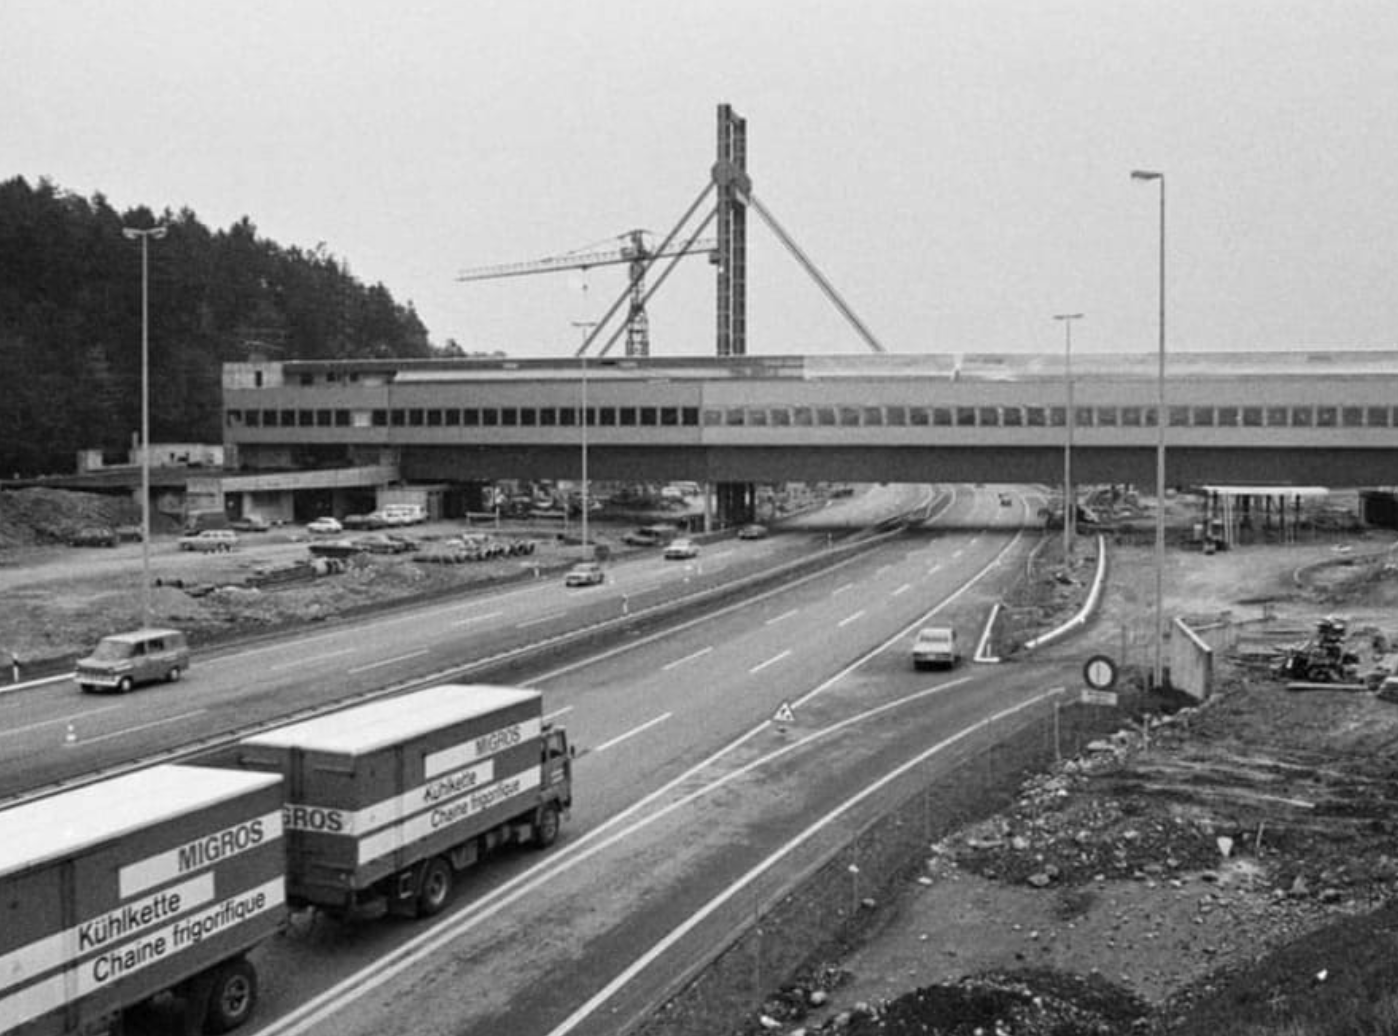
\includegraphics[width=0.8\linewidth]{images/fressbalken_wuerenlos.png}
\end{center}

\subsection{Zentrale Erkenntnisse}

Die Geschichte des Automobils ist keine reine Erfolgsgeschichte technischer Innovation.

Sie zeigt:

\begin{itemize}
    \item den Übergang von der Industrie- zur Konsumgesellschaft
    \item die Bedeutung der Massenproduktion
    \item die Verbindung von Mobilität und individueller Freiheit
    \item die globale Verflechtung industrieller Produktion
    \item die Rolle von Kontrolle und Disziplinierung in modernen Gesellschaften
\end{itemize}

Die zentrale These lautet:

Die moderne Automobilgesellschaft entstand nicht allein durch technische Erfindungen.
Sie wurde durch neue Produktionsformen,
globale Rohstoffketten,
Konsumpraktiken und gesellschaftliche Leitbilder von Freiheit ermöglicht.
        \section{Der „neue Mensch“ und die Technisierung des Haushalts}

\subsection{Einführung: Rationalisierung als gesellschaftliches Leitbild}

Die Vorlesung untersucht die Ausweitung technischer und wissenschaftlicher
Rationalisierung auf immer neue Bereiche des gesellschaftlichen Lebens.

Während Rationalisierung zunächst vor allem mit industrieller Produktion
verbunden war, entstand im Verlauf des 19. und 20. Jahrhunderts die Vorstellung,
dass auch Menschen, Lebensweisen und soziale Strukturen
wissenschaftlich gestaltet und optimiert werden könnten.

Grundlage dafür war ein tiefes Vertrauen in Wissenschaft,
Technik und Fortschritt.

Diese galten als objektive Instrumente,
mit deren Hilfe sich gesellschaftliche Probleme lösen
und die Lebensbedingungen verbessern liessen.

Zentrale Leitfragen:

\begin{itemize}
    \item Wie wurde der Mensch selbst zum Gegenstand technischer Planung?
    \item Welche Vorstellungen von Fortschritt prägten das 20. Jahrhundert?
    \item Wie beeinflussten Wissenschaft und Technik Alltag und Lebensführung?
    \item Weshalb wurde auch der Haushalt rationalisiert?
\end{itemize}

Die Geschichte der Technisierung des Haushalts ist daher nicht nur
Technikgeschichte, sondern auch Sozial-, Kultur- und Ideengeschichte.

\subsection{Industrialisierungserfahrungen und die Idee der gesellschaftlichen Optimierung}

Die Industrialisierung führte nicht nur zu wirtschaftlichen Veränderungen,
sondern auch zu neuen gesellschaftspolitischen Vorstellungen.

Viele Reformbewegungen gingen davon aus,
dass Wissenschaft und Technik genutzt werden könnten,
um Individuen und Gesellschaft gezielt zu verbessern.

Zu den wichtigsten Strömungen gehörten:

\begin{itemize}
    \item Eugenik
    \item Lebensreform
    \item die Vorstellung des „neuen Menschen“
\end{itemize}

Obwohl sich diese Bewegungen stark unterschieden,
teilten sie die Annahme,
dass gesellschaftlicher Fortschritt durch Planung,
Steuerung und Optimierung erreicht werden könne.

\subsection{Eugenik und die wissenschaftliche Steuerung des Menschen}

Die Eugenik verstand sich als wissenschaftlich begründetes Programm
zur Verbesserung der Gesellschaft durch die Kontrolle menschlicher Fortpflanzung.

Typische Massnahmen waren:

\begin{itemize}
    \item Eheverbote
    \item Zwangssterilisationen
    \item Gesundheits- und Hygienekampagnen
    \item Förderung bestimmter Bevölkerungsgruppen
\end{itemize}

Die Eugenik verband Wissenschaft,
Politik und Moral zu einem System gesellschaftlicher Steuerung.

Ziel war die Schaffung eines gesunden,
leistungsfähigen und produktiven „Volkskörpers“.

Heute gilt die Eugenik als Beispiel dafür,
wie wissenschaftliche Autorität zur Legitimation
von Diskriminierung und Gewalt eingesetzt werden konnte.

\begin{center}
    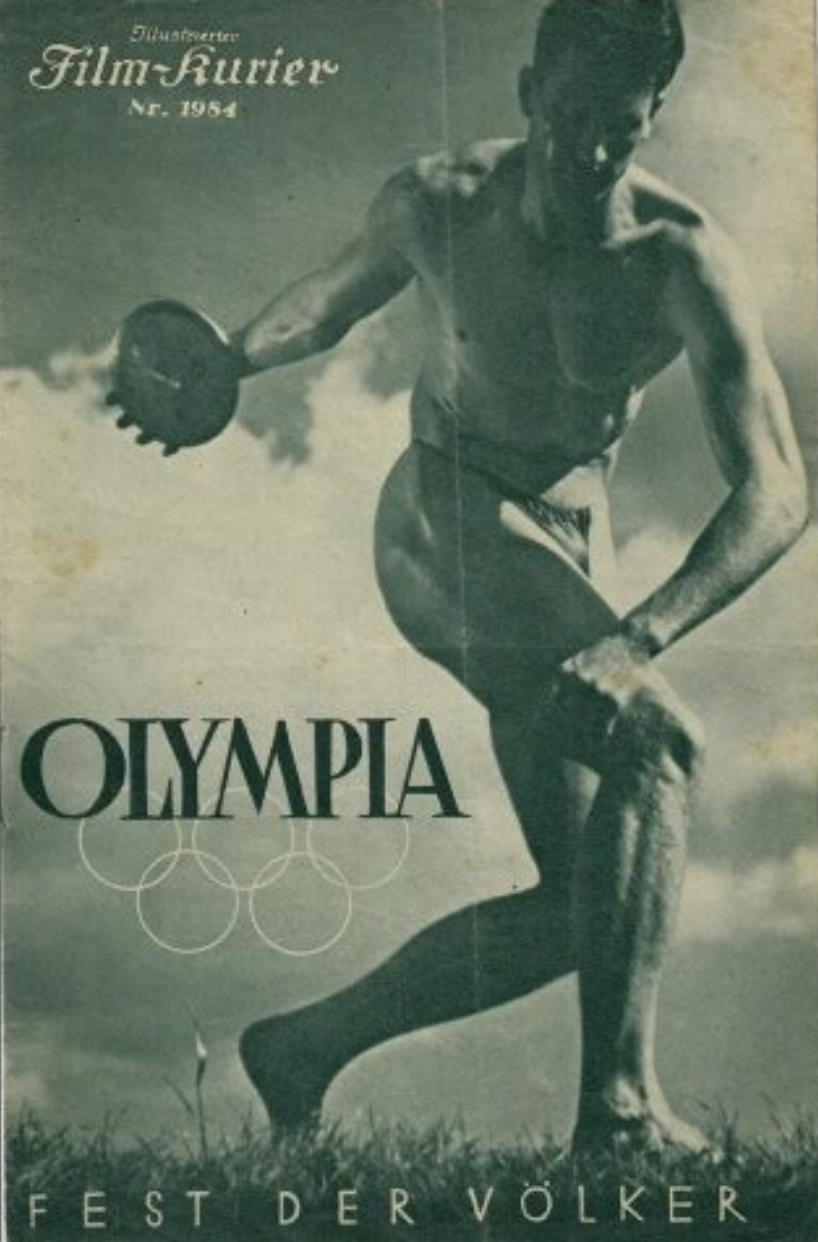
\includegraphics[width=0.55\linewidth]{images/olympia_1936.png}
\end{center}

\subsection{Lebensreform und die Suche nach dem natürlichen Leben}

Parallel zur Eugenik entwickelte sich die Lebensreformbewegung.

Sie kritisierte die Folgen von Industrialisierung,
Urbanisierung und Massenkonsum.

Angestrebt wurden:

\begin{itemize}
    \item gesunde Ernährung
    \item Körperkultur und Sport
    \item Naturheilkunde
    \item naturnahe Lebensformen
\end{itemize}

Die Bewegung verstand sich als Gegenentwurf
zur modernen Industriegesellschaft.

Gleichzeitig beruhte auch sie auf der Vorstellung,
dass Menschen und Gesellschaft gezielt verbessert
und optimiert werden könnten.

Dadurch weist sie trotz ihrer Kritik an der Moderne
Parallelen zu anderen Rationalisierungsprojekten auf.

\begin{center}
    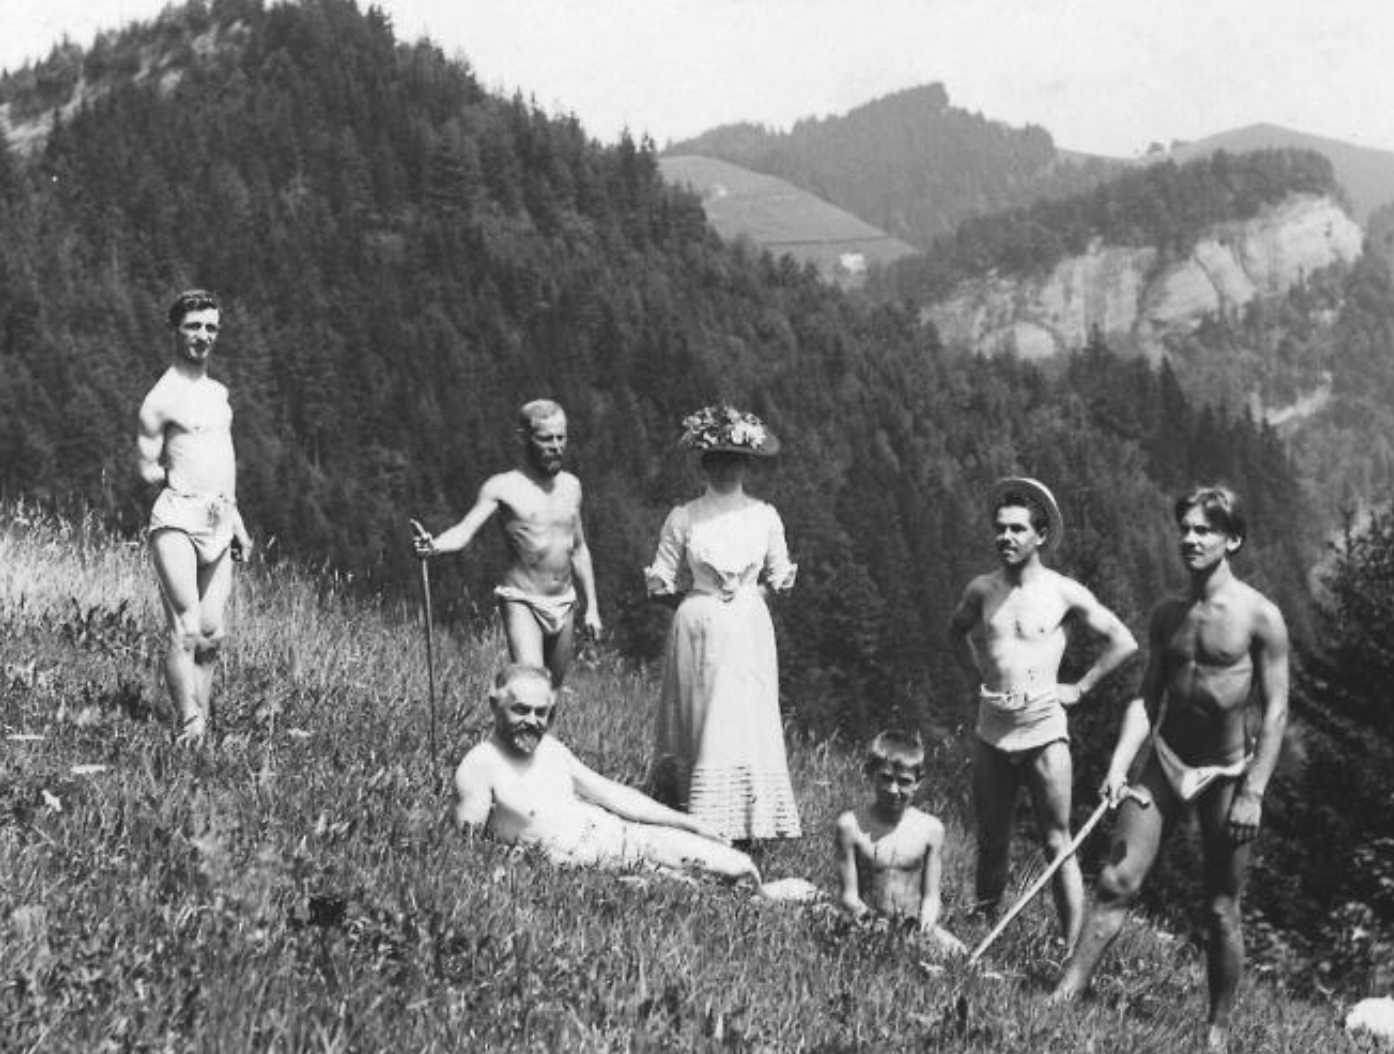
\includegraphics[width=0.8\linewidth]{images/monte_verita.png}
\end{center}

\subsection{Der „neue Mensch“ als gesellschaftliches Ideal}

Besonders im sozialistischen Denken entstand die Vorstellung
eines „neuen Menschen“.

Dieser sollte nicht nur technisch ausgebildet,
sondern auch moralisch, sozial und politisch
den Anforderungen einer zukünftigen Gesellschaft entsprechen.

Dazu dienten unter anderem:

\begin{itemize}
    \item Bildung und Erziehung
    \item Gesundheitsprogramme
    \item Arbeitsorganisation
    \item Freizeit- und Kulturangebote
\end{itemize}

Technischer Fortschritt,
gesellschaftlicher Fortschritt und moralische Entwicklung
wurden dabei als untrennbare Einheit verstanden.

Die Optimierung des Menschen galt zugleich
als Optimierung der Gesellschaft.

\begin{center}
    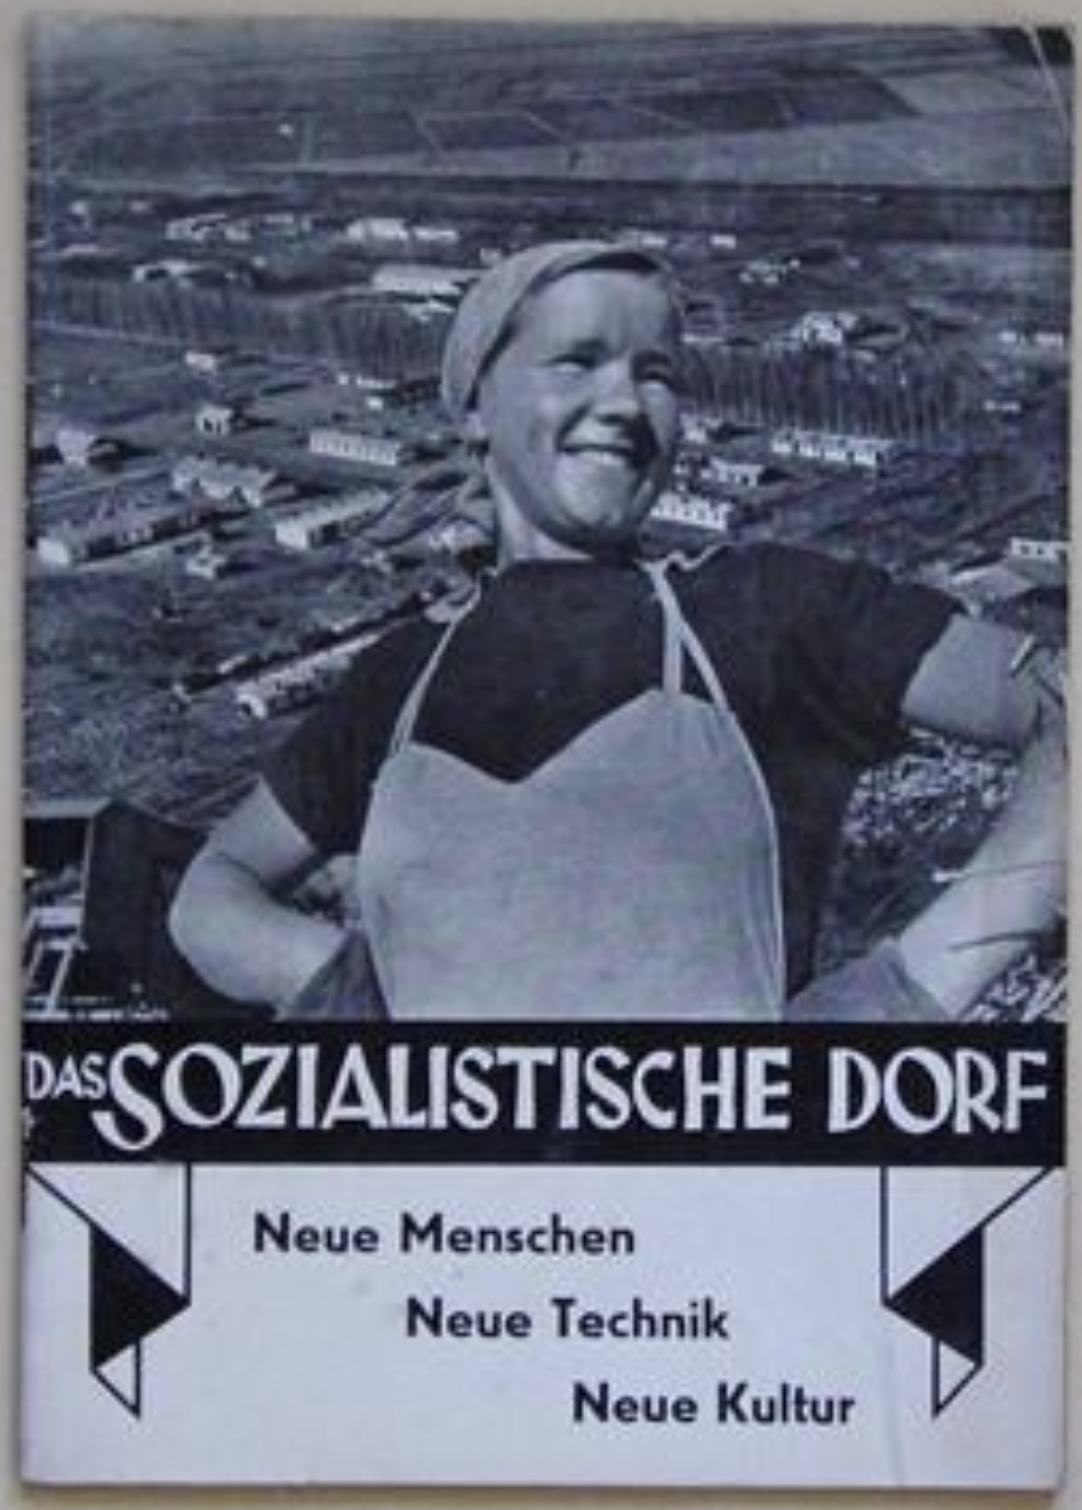
\includegraphics[width=0.55\linewidth]{images/sozialistisches_dorf.png}
\end{center}

\subsection{Technik, Wissenschaft und soziale Kontrolle}

Die Vorlesung zeigt,
dass Wissenschaft und Technik im 20. Jahrhundert
zunehmend als Instrumente gesellschaftlicher Steuerung eingesetzt wurden.

Menschen wurden vermessen,
klassifiziert und analysiert.

Dazu gehörten:

\begin{itemize}
    \item Körperstudien
    \item Bewegungsanalysen
    \item Leistungsmessungen
    \item medizinische und genetische Untersuchungen
\end{itemize}

Wissenschaftliche Erkenntnisse erschienen dadurch objektiv und neutral.

Tatsächlich waren sie jedoch häufig eng mit politischen,
gesellschaftlichen und moralischen Zielvorstellungen verbunden.

Technik strukturierte Verhalten zunehmend,
ohne dass direkter Zwang notwendig war.

\subsection{Rationalisierung des Wohnens}

Die Prinzipien der Rationalisierung beschränkten sich nicht auf Fabriken.

Auch Wohnräume wurden zum Gegenstand technischer Planung.

Ausgangspunkt waren:

\begin{itemize}
    \item Wohnungsnot
    \item Verstädterung
    \item neue Vorstellungen von Hygiene
    \item funktionale Architektur
\end{itemize}

Die Architektur der Neuen Sachlichkeit
forderte zweckmässige und effizient gestaltete Wohnungen.

Wohnräume wurden neu organisiert,
Arbeitsabläufe vereinfacht
und traditionelle Wohnformen verändert.

\begin{center}
    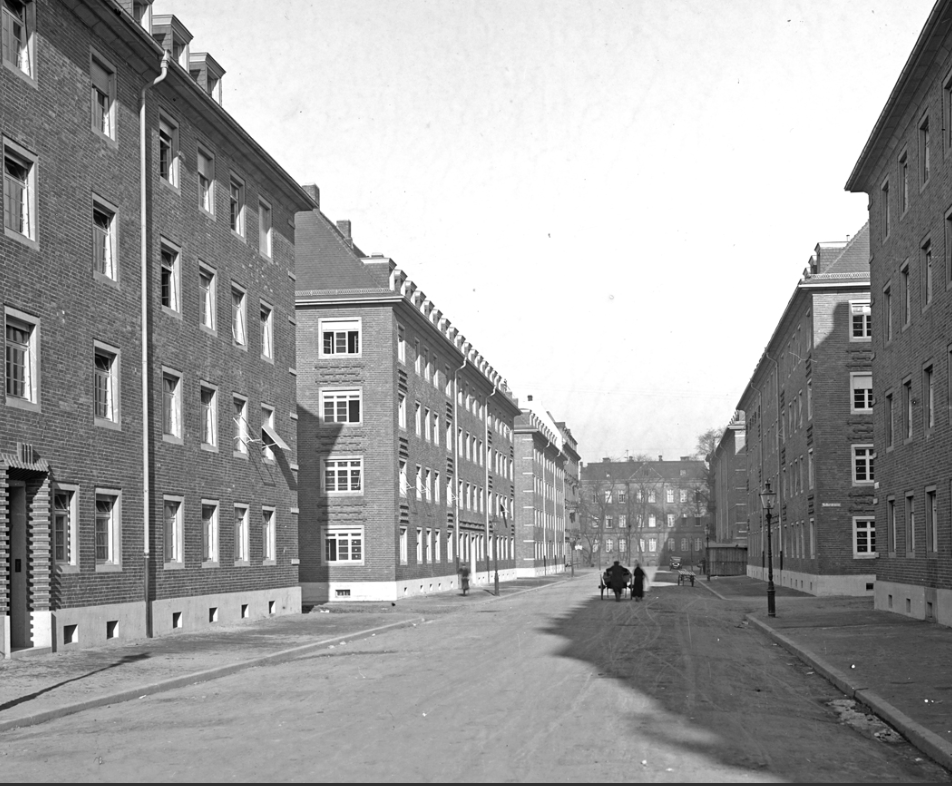
\includegraphics[width=0.85\linewidth]{images/wohnungsnot_moderner_wohnblock.png}
\end{center}

\subsection{Die Frankfurter Küche}

Ein besonders bekanntes Beispiel
für die Rationalisierung des Alltags
ist die Frankfurter Küche von Margarete Schütte-Lihotzky.

Sie wurde ab 1926 entwickelt
und orientierte sich an den Prinzipien
wissenschaftlicher Arbeitsorganisation.

Ziel war die Reduktion unnötiger Wege
und die Effizienzsteigerung der Hausarbeit.

Die Küche wurde als funktionaler Arbeitsraum gestaltet,
dessen Aufbau auf Bewegungsanalysen beruhte.

Damit übertrug man die Logik industrieller Rationalisierung
auf den privaten Haushalt.

\begin{center}
    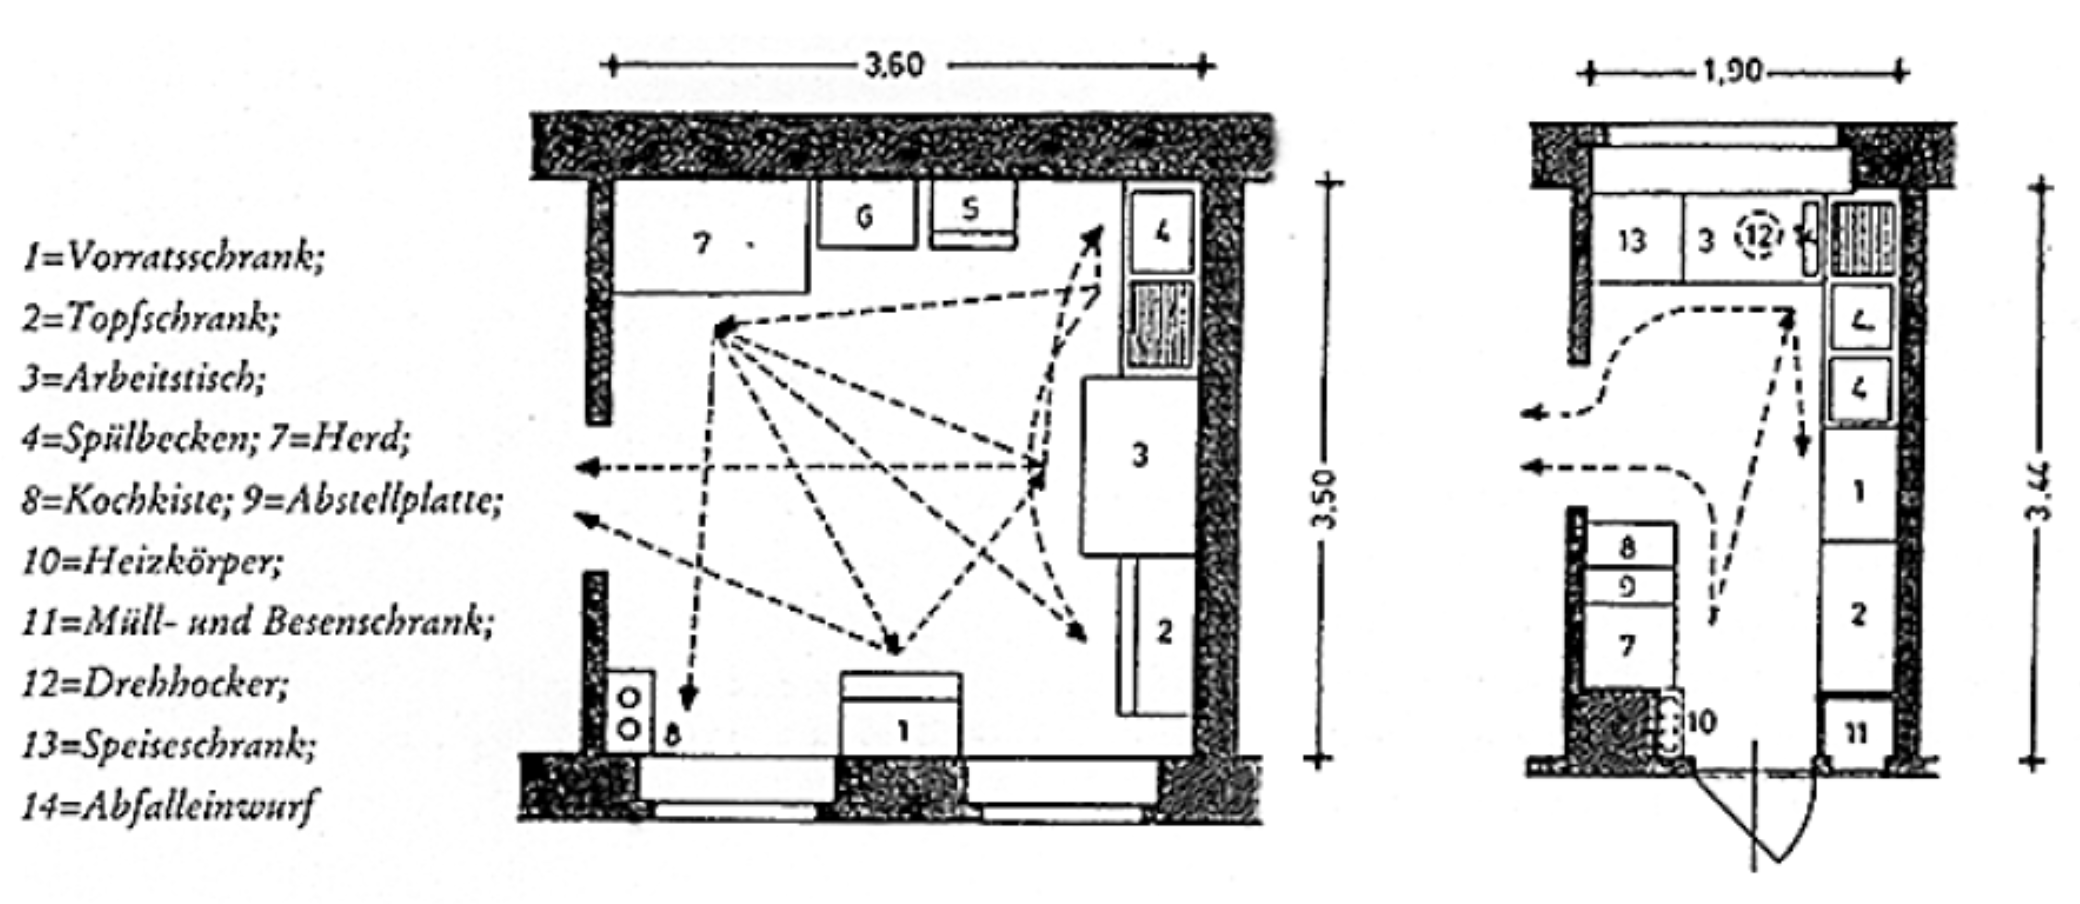
\includegraphics[width=0.9\linewidth]{images/frankfurter_kueche.png}
\end{center}

\subsection{Emanzipation und Kontrolle}

Die Rationalisierung des Alltags besitzt eine doppelte Bedeutung.

Einerseits versprach sie:

\begin{itemize}
    \item höheren Lebensstandard
    \item bessere Hygiene
    \item gesundheitliche Verbesserungen
    \item Arbeitserleichterungen
\end{itemize}

Andererseits führte sie zu neuen Formen
gesellschaftlicher Kontrolle und Normierung.

Die Soziologen Max Horkheimer und Theodor W. Adorno
kritisierten diese Entwicklung als „instrumentelle Vernunft“.

Sie warnten davor,
dass Rationalität zunehmend zum Instrument
der Kontrolle von Menschen und Gesellschaft werde.

Die Geschichte der Technisierung des Haushalts
bewegt sich daher stets im Spannungsfeld
zwischen Befreiung und Kontrolle.

\subsection{Zentrale Erkenntnisse}

Die Vorlesung zeigt,
dass technische Rationalisierung weit über Fabriken hinauswirkte.

Sie beeinflusste:

\begin{itemize}
    \item Vorstellungen von Gesundheit
    \item Erziehung und Bildung
    \item Wohnformen
    \item Haushaltsführung
    \item gesellschaftliche Normen
\end{itemize}

Die zentrale These lautet:

Die Technisierung des Haushalts ist Teil eines umfassenden historischen Prozesses,
in dem Wissenschaft und Technik nicht nur Maschinen,
sondern auch Menschen, Lebensweisen und soziale Strukturen
gestalten sollten.

Dabei entstanden sowohl neue Freiheiten
als auch neue Formen gesellschaftlicher Kontrolle.
        \section{Lesende und rechnende Kassen: Von der Industrie- zur Konsumgesellschaft}

\subsection{Einführung: Technik im Übergang zur Konsumgesellschaft}

Die Vorlesung untersucht den historischen Übergang
von der Industriegesellschaft zur Konsumgesellschaft.

Während Technik im 19. und frühen 20. Jahrhundert
vor allem mit industrieller Produktion,
Fabriken und Arbeitsorganisation verbunden war,
verlagerte sie sich im Verlauf des 20. Jahrhunderts
zunehmend in den Alltag.

Technik organisierte nun nicht mehr nur Arbeit,
sondern auch Konsum,
Haushaltsführung,
Wohnformen und Geschlechterrollen.

Zentrale Leitfragen:

\begin{itemize}
\item Wie verändert Technik den Alltag ausserhalb der Fabrik?
\item Welche Rolle spielte der Haushalt im Übergang zur Konsumgesellschaft?
\item Wie entstanden neue Konsumnormen und Vorstellungen vom richtigen Leben?
\item Wie veränderten technische Geräte die Rolle der Hausfrau?
\item Was zeigt der Strichcode über Konsum und Rationalisierung in den 1970er Jahren?
\end{itemize}

Die Geschichte lesender und rechnender Kassen
ist daher nicht nur eine Geschichte technischer Innovation,
sondern auch eine Geschichte gesellschaftlicher Ordnung,
des Konsums und der Veränderung alltäglicher Praktiken.

\subsection{Die Frankfurter Küche als rationalisierter Privatraum}

Die Vorlesung knüpft anschliessend
an die Rationalisierung des Haushalts an.

Ein wichtiges Beispiel dafür ist erneut
die Frankfurter Küche.

Sie entstand im Zusammenhang
mit der Wohnreform der Neuen Sachlichkeit.

Diese Reformbewegung verfolgte das Ziel,
Wohnräume funktional,
zweckmässig und hygienisch zu gestalten.

Die Frankfurter Küche wurde ab den 1920er Jahren entwickelt
und verbreitete sich später auch ausserhalb Deutschlands,
besonders in den 1950er Jahren.

Sie übertrug Prinzipien des scientific management
auf den privaten Wohnraum.

Ziele waren:

\begin{itemize}
\item Entlastung der Hausarbeit
\item mehr Komfort
\item hygienische Verbesserung
\item effizientere Arbeitsabläufe
\item Modernisierung des Alltags
\end{itemize}

Besonders im Wohnungsbau für Arbeiterfamilien
galt funktionaler Wohnungsbau
als erstrebenswerte Verbesserung
der Wohn- und Lebensverhältnisse.

\begin{center}
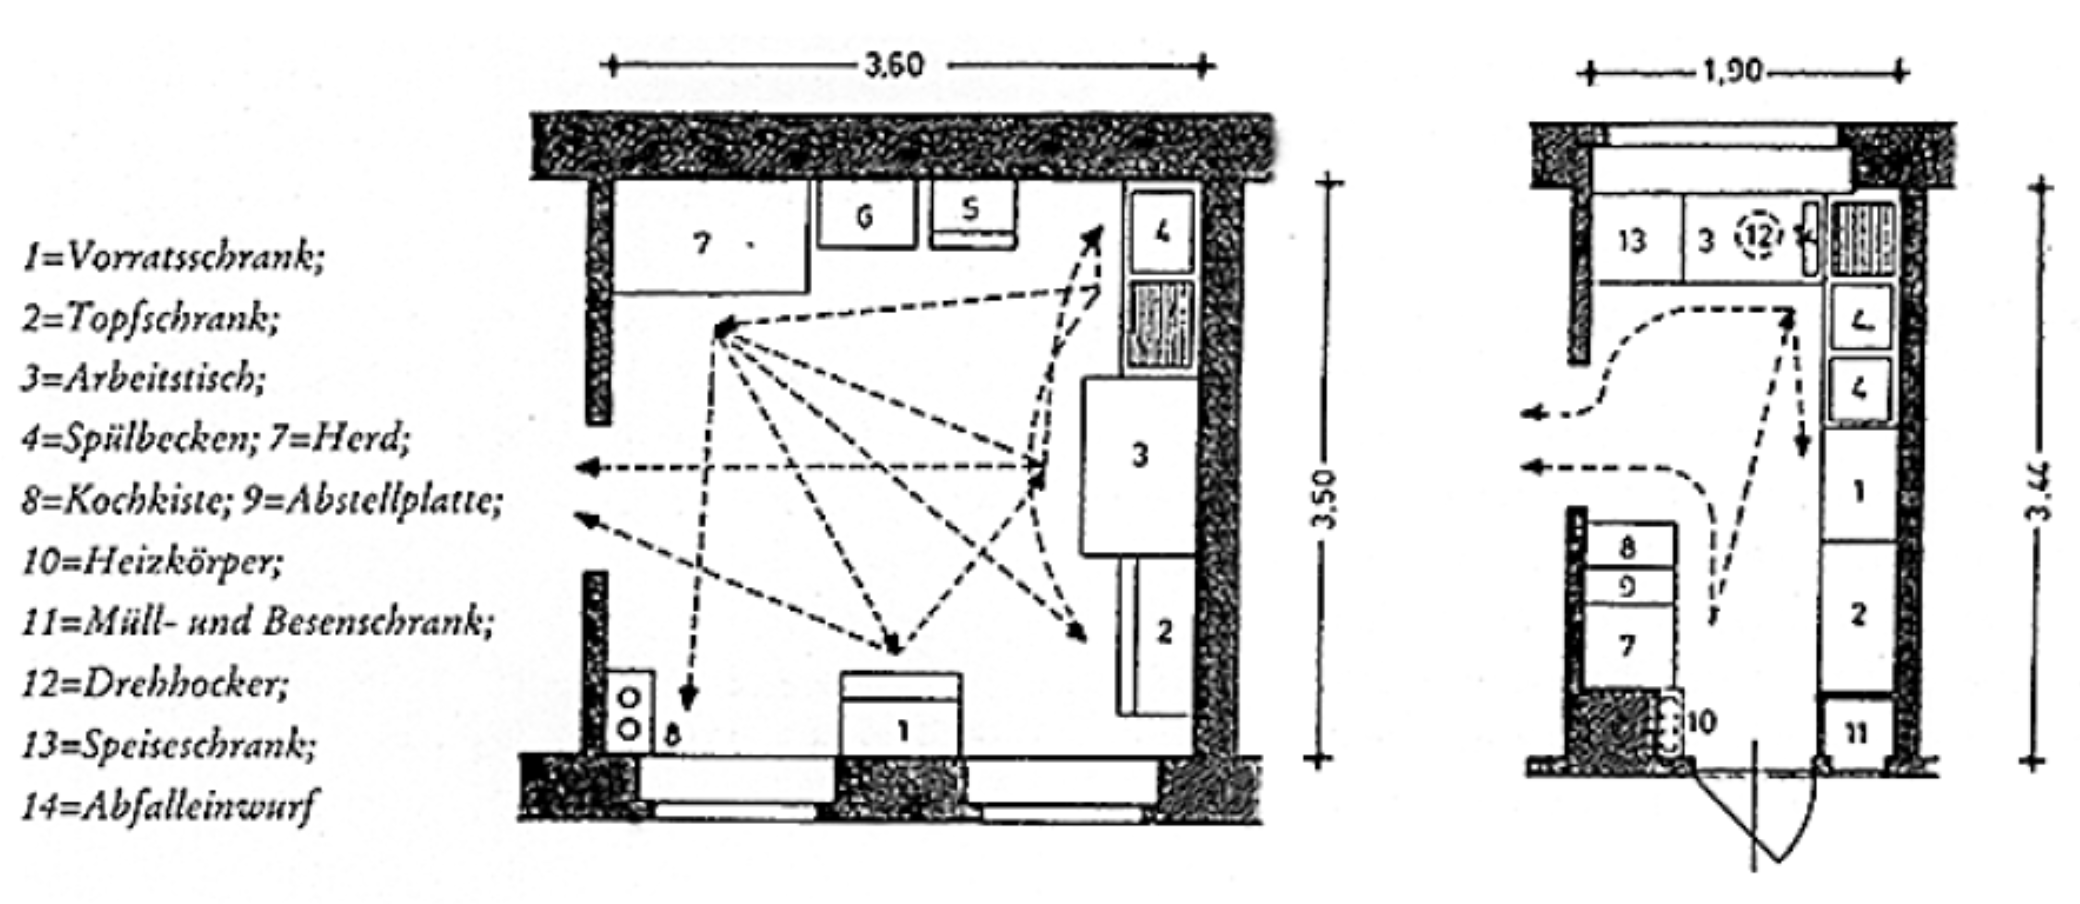
\includegraphics[width=0.85\linewidth]{images/frankfurter_kueche.png}
\end{center}

\subsection{Die Küche, das Heim und die Hausfrau}

Das neue Wohnkonzept ordnete jedem Raum
eine bestimmte Funktion zu.

Damit wurde nicht nur festgelegt,
wie Räume genutzt werden sollten,
sondern auch,
wer sich in ihnen aufhalten sollte.

Die Frankfurter Küche war als Arbeitsraum
für eine einzelne Person konzipiert.

Diese Person war in der gesellschaftlichen Vorstellung
die Hausfrau.

Die Architektur zwang die Bewohnerinnen und Bewohner
zwar nicht unmittelbar dazu,
entsprechend dieser Ordnung zu leben.

Sie legte jedoch bestimmte Verhaltensweisen nahe.

Die Küche wurde dadurch zu einem Raum,
in dem sich gesellschaftliche Vorstellungen
von Geschlecht,
Arbeit und Ordnung materialisierten.

Wichtig ist jedoch:
Die Figur der Frau als Managerin des Haushalts
entstand nicht erst durch diese baulichen Massnahmen.

Sie existierte bereits zuvor
und wurde durch die neue Wohnarchitektur
weiter stabilisiert.

\subsection{Der „Oikos“ als vormoderner Haushalt}

Um die moderne Hausfrau historisch einordnen zu können,
blickt die Vorlesung auf den vormodernen Haushalt zurück.

Vor der Industrialisierung,
also bis ins 18. Jahrhundert,
war der Haushalt nicht nur Wohnort,
sondern zugleich Arbeitsstätte.

Er bildete eine kleine,
relativ ganzheitliche Wirtschaftseinheit.

Der Haushalt war weitgehend auf Selbstversorgung ausgerichtet.

Viele Dinge,
die für das tägliche Leben gebraucht wurden,
wurden selbst hergestellt oder produziert.

Dazu gehörten unter anderem:

\begin{itemize}
\item Feldarbeit
\item Ernte
\item Viehhaltung
\item Nähen von Kleidern
\item Waschen und Putzen
\item Kochen
\item Haltbarmachen von Lebensmitteln
\end{itemize}

Auch in der Vormoderne waren Arbeiten
geschlechtlich zugeordnet.

Dennoch beteiligten sich grundsätzlich
alle im Haushalt lebenden Personen
in irgendeiner Form an der Hausarbeit.

Der Hausherr repräsentierte den Haushalt nach aussen,
während die Hausmutter die Arbeit organisierte.

\begin{center}
\includegraphics[width=0.5\linewidth]{images/oikos.png}
\end{center}

\subsection{Die Hausfrau als Erfindung des 19. Jahrhunderts}

Mit der Industrialisierung veränderte sich
die Struktur des Haushalts grundlegend.

Produktion und Reproduktion wurden zunehmend getrennt.

Die Fabrik wurde zum Ort der Erwerbsarbeit,
das Haus zum Ort der Reproduktion,
Kindererziehung und Haushaltsführung.

Dadurch entstanden ein öffentlicher
und ein privater Raum,
die klar voneinander unterschieden wurden.

Als gesellschaftliche Norm setzte sich zunehmend
folgendes Familienmodell durch:

\begin{itemize}
\item Der Mann arbeitet ausser Haus als Lohnarbeiter oder Erwerbstätiger.
\item Er gilt als Ernährer der Familie.
\item Die Frau bleibt im Haus.
\item Sie zieht die Kinder auf und führt den Haushalt.
\end{itemize}

Die Arbeit der Frau und Mutter
wurde dabei nicht entlohnt.

Gleichzeitig wurde sie moralisch stark aufgeladen.

Die gute Hausfrau wurde zum Ideal
einer geordneten,
modernen und bürgerlichen Lebensweise.

\subsection{Technisierung des Haushalts ab den 1920er Jahren}

Ab den 1920er Jahren kamen vermehrt technische Geräte
für den Haushalt auf den Markt.

Dazu gehörten:

\begin{itemize}
\item Staubsauger
\item Backöfen
\item Waschmaschinen
\item elektrische Lampen
\item weitere elektrische Haushaltsgeräte
\end{itemize}

Als Konsumgüter für breite Bevölkerungsschichten
wurden diese Geräte jedoch erst nach dem Zweiten Weltkrieg
wirklich erschwinglich.

Mit technischen Geräten sollte der Haushalt
effizienter geführt werden.

Ähnlich wie in der Fabrik
kam es auch im Haushalt
zu einer Reorganisation von Arbeit.

Die Technisierung brachte neue Normen,
Zielsetzungen und Erwartungen hervor.

Der Haushalt sollte sauberer,
moderner,
rationeller und besser organisiert sein.

\begin{center}
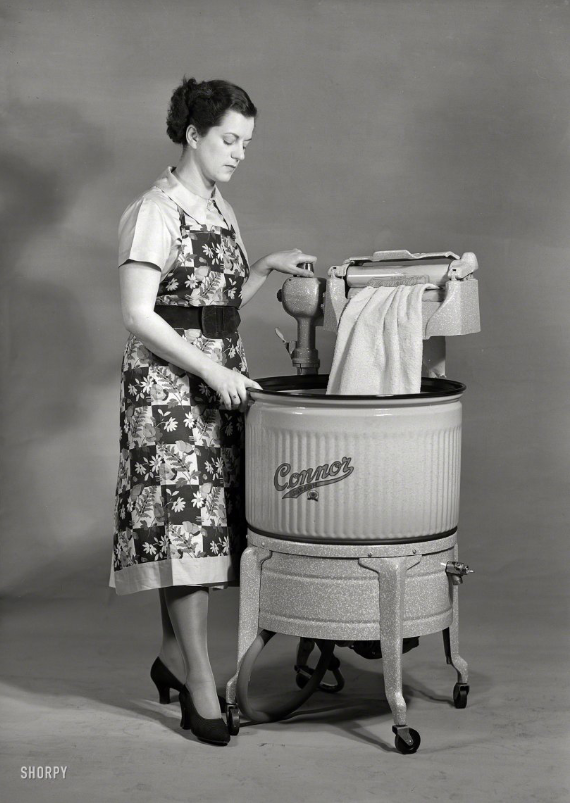
\includegraphics[width=0.5\linewidth]{images/Technik_im_Haushalt.png}
\end{center}

\subsection{Entlastung, Isolation und Geschlechterrollen}

Technische Geräte versprachen zunächst
eine deutliche Entlastung.

Sie konnten körperlich anstrengende Arbeiten
vereinfachen oder beschleunigen.

Besonders die Hausfrau sollte dadurch
von schwerer körperlicher Arbeit entlastet werden.

Gleichzeitig führte die Technisierung des Haushalts
aber auch zu neuen Formen der Isolation.

Hausarbeit wurde weniger in Kooperation
und Gemeinschaft verrichtet.

Stattdessen arbeitete die Hausfrau zunehmend allein
mit technischen Geräten im privaten Raum.

Technik stabilisierte damit bestehende Geschlechterrollen.

Sie machte den Haushalt effizienter,
stellte aber die geschlechtliche Zuständigkeit
für diese Arbeit nicht grundsätzlich in Frage.

Die Vorlesung betont jedoch,
dass die Stabilisierung von Geschlechterrollen
durch Technik kontextabhängig ist.

Technik besitzt kein festes Geschlecht.

Ihre gesellschaftliche Bedeutung entsteht erst
durch konkrete Arbeitsverhältnisse,
Eigentumsformen,
Körperbilder und kulturelle Zuschreibungen.

%\begin{center}
%\includegraphics[width=0.65\linewidth]{images/waschmaschine_1950.png}
%\end{center}

\subsection{Technik und Geschlecht}

Die Vorlesung zeigt anhand verschiedener Beispiele,
dass Geschlecht \textbf{nicht} einfach in Technik eingeschrieben ist.

Technische Geräte sind \textbf{nicht} von sich aus männlich oder weiblich.

Erst ihre Nutzung,
ihre soziale Einbettung
und ihre ökonomische Bedeutung
machen sie zu geschlechtlich codierten Objekten.

Beim Maschinensticken führte der Einsatz von Maschinen dazu,
dass Männer in einem Bereich tätig wurden,
der zuvor stark mit weiblicher Handarbeit verbunden war.

Dies hing unter anderem damit zusammen,
dass Maschinensticken kapitalintensiv war
und Besitz,
Wartung und körperliche Belastung erforderte.

Bei der Schreibarbeit verlief die Entwicklung anders.

Durch die Schreibmaschine wurde Büro- und Sekretariatsarbeit
zunehmend feminisiert.

Diese Arbeit wurde zugleich abgewertet
und schlechter entlohnt.

Daran zeigt sich:

Nicht die Technik selbst bestimmt Geschlechterrollen,
sondern ihre gesellschaftliche Organisation.

%\begin{center}
%\includegraphics[width=0.8\linewidth]{images/technik_und_geschlecht.png}
%\end{center}

\subsection{Technisierung des Haushalts ab den 1950er Jahren}

Ab den 1950er Jahren wurden technische Geräte
zunehmend zu Konsumgütern.

Der Haushalt wurde dadurch zu einem wichtigen Markt.

Die durch Technik stabilisierte Figur der Hausfrau
wurde nun zugleich zur Konsumentin.

Werbung und Produktdesign richteten sich
an ihre vermeintlichen Bedürfnisse.

Gleichzeitig schufen sie diese Bedürfnisse
aber auch erst mit.

Waschmittel,
Küchengeräte,
Staubsauger,
Kühlschränke und andere Produkte
wurden nicht nur als praktische Hilfen verkauft,
sondern als Zeichen eines modernen,
richtigen und gepflegten Haushalts.

Dadurch entstanden neue Normen darüber,
wie ein Haushalt geführt werden sollte.

Besonders wichtig wurden Erwartungen an:

\begin{itemize}
\item Hygiene
\item Sauberkeit
\item Ausstattung
\item Ordnung
\item Dekoration
\item Modernität
\end{itemize}

Die Hausfrau wurde damit zur zentralen Figur
der Konsumgesellschaft.

Sie war verantwortlich für den Kauf,
die Nutzung und die Bewertung technischer Konsumgüter
im privaten Alltag.

%\begin{center}
%\includegraphics[width=0.55\linewidth]{images/persil_werbung_1950er.png}
%\end{center}

\subsection{Der Strichcode und die Rationalisierung des Konsums}

Ein weiteres Thema der Vorlesung ist der Strichcode,
der in den 1970er Jahren
als neue Kassentechnologie diskutiert wurde.

Die Quelle zum Strichcode von 1973 zeigt,
wie technische Rationalisierung
auch den Bereich des Einkaufens erfasste.

Die Kasse wurde nicht mehr nur als Ort des Bezahlens verstanden,
sondern als Schnittstelle zwischen Ware,
Information,
Preis,
Verkauf und Konsumverhalten.

Der Strichcode versprach:

\begin{itemize}
\item schnelleres Kassieren
\item genauere Preisberechnung
\item bessere Warenkontrolle
\item effizientere Lagerhaltung
\item Rationalisierung des Detailhandels
\end{itemize}

Damit wurde eine Logik,
die zuvor vor allem aus Fabrik und Verwaltung bekannt war,
auf den Konsum übertragen.

Nicht nur die Produktion,
sondern auch der Einkauf wurde messbar,
standardisiert und berechenbar.

Die lesende und rechnende Kasse steht daher
für eine neue Phase der Konsumgesellschaft.

Konsum wurde technisch organisiert,
statistisch erfassbar
und ökonomisch besser steuerbar.
\begin{center}
\includegraphics[width=0.8\linewidth]{images/barcode.png}
\end{center}

\subsection{Von der Industrie- zur Konsumgesellschaft}

Die zentrale These der Vorlesung lautet,
dass sich Technik im 20. Jahrhundert
zunehmend vom industriellen Produktionsbereich
in den Alltag verlagerte.

In der Industrie organisierte Technik Arbeit.

Im Haushalt organisierte sie Lebensweisen,
Konsumpraktiken und Geschlechterrollen.

Die Hausfrau war ein Produkt der Moderne.

Sie stand im Zentrum eines technisierten Alltags,
der weniger auf Produktion
als auf Konsum und Reproduktion ausgerichtet war.

Technische Geräte,
Werbung,
Produktdesign,
Wohnarchitektur und Kassensysteme
wirkten gemeinsam an der Entstehung
moderner Konsumgesellschaften mit.

In der Konsumgesellschaft wurden Technik
und Technikfolgen zudem zunehmend
zu Themen des öffentlichen Lebens und der Politik.

Dazu gehörten Fragen nach:

\begin{itemize}
\item Umwelt
\item Infrastruktur
\item Deindustrialisierung
\item Konsumkritik
\item sozialer Ordnung
\end{itemize}

\subsection{Zentrale Erkenntnisse}

Die Vorlesung zeigt,
dass Technik nicht nur Maschinenarbeit
in Fabriken veränderte.

Sie prägte auch den privaten Alltag,
die Organisation des Haushalts
und die Entstehung moderner Konsumformen.

Zentrale Erkenntnisse sind:

\begin{itemize}
\item Die moderne Hausfrau entstand im Zusammenhang mit der Trennung von Produktion und Reproduktion.
\item Haushaltsgeräte versprachen Entlastung, stabilisierten aber häufig bestehende Geschlechterrollen.
\item Technik ist nicht von sich aus geschlechtlich, sondern wird in bestimmten sozialen Kontexten geschlechtlich codiert.
\item Ab den 1950er Jahren wurde der Haushalt zu einem zentralen Ort des Konsums.
\item Werbung und Produktdesign schufen neue Bedürfnisse und Normen des richtigen Haushalts.
\item Der Strichcode zeigt, wie Rationalisierung auch den Einkauf und den Konsum erfasste.
\end{itemize}

Die zentrale These lautet:

Der Übergang von der Industrie- zur Konsumgesellschaft
bedeutete nicht das Ende technischer Rationalisierung.

Vielmehr verlagerte sie sich in neue Bereiche.

Technik strukturierte nun nicht mehr nur Produktion und Arbeit,
sondern auch Konsum,
Haushalt,
Geschlechterrollen und alltägliche Lebensführung.

        \section{Zum Mensch-Maschinen-Verhältnis: Kleine Geschichte der KI}

\subsection{Einführung: Technikentwicklung und Mensch-Maschinen-Verhältnis}

Die Vorlesung untersucht das Verhältnis von Mensch und Maschine
am Beispiel der Geschichte der Künstlichen Intelligenz.

Im Zentrum steht dabei nicht nur die technische Entwicklung von KI,
sondern auch die Frage,
welche Vorstellungen vom Menschen
in technischen Systemen und Erklärungen von Technikentwicklung enthalten sind.

Die Geschichte der KI ist daher nicht nur eine Geschichte
von Computern,
Programmen und Algorithmen.

Sie ist zugleich eine Geschichte darüber,
wie Menschen ihre eigenen Fähigkeiten,
Grenzen und Fehler im Vergleich zu Maschinen verstehen.

Zentrale Leitfragen:

\begin{itemize}
\item Warum entwickeln Menschen Technik?
\item Welche Vorstellungen vom Menschen liegen Technikentwicklung zugrunde?
\item Weshalb erscheinen Maschinen oft als überlegen?
\item Welche Rolle spielt menschliche Fehlbarkeit in der Technikgeschichte?
\item Was verändert KI am Verhältnis von Mensch und Maschine?
\end{itemize}

Die Vorlesung zeigt,
dass Technikentwicklung immer auch mit Hoffnungen,
Ängsten,
Machtvorstellungen und Menschenbildern verbunden ist.

\subsection{Effekte der Technikentwicklung seit 1800}

Seit etwa 1800 veränderte Technik
die Lebensbedingungen grosser Teile der Bevölkerung grundlegend.

Technische Entwicklung führte zu höherer Produktivität,
neuen Produktionsweisen
und wachsendem Wohlstand für viele Menschen.

Sie trug dazu bei,
den Lebensstandard zu erhöhen
und die Abhängigkeit von unmittelbarer Subsistenzwirtschaft zu verringern.

Lebensmittelproduktion,
Mobilität,
Kommunikation,
Bildung und Arbeit wurden zunehmend technisch organisiert.

Wichtige Effekte waren:

\begin{itemize}
\item höhere Produktivität
\item mehr Wohlstand für grosse Teile der Bevölkerung
\item Erhöhung des Lebensstandards
\item Überproduktion von Lebensmitteln
\item Alphabetisierung und Bildung
\item neue Formen politischer und gesellschaftlicher Teilhabe
\end{itemize}

Gleichzeitig veränderte Technik auch die Lebensweise
und Arbeitsweise der Menschen.

Der Alltag wurde neu strukturiert.

Die Trennung von Arbeiten und Wohnen,
die Entstehung der Fabrik,
neue Tagesabläufe
und neue Formen von Lohnarbeit
prägten moderne Gesellschaften.

\subsection{Technik, Gesellschaft und neue Organisationsformen}

Technikentwicklung seit 1800 führte nicht nur
zu neuen Maschinen,
sondern auch zu neuen Organisationsformen.

Fabriken,
Fabrikordnungen,
Fliessbandarbeit,
Management,
Spezialisierung
und Informationsverarbeitung
veränderten die Art,
wie Menschen arbeiteten und zusammenlebten.

Dabei entstanden auch neue gesellschaftliche Figuren.

Dazu gehörten:

\begin{itemize}
\item Unternehmer
\item Fabrikarbeiter und Proletariat
\item Fabrikanten
\item Angestellte
\item Manager
\end{itemize}

Zugleich entstanden neue politische Ideologien
und gesellschaftliche Bewegungen.

Sozialismus,
Marxismus,
Kapitalismus,
Liberalismus,
Sozialdemokratie,
Frauenrechtsbewegung
und Faschismus
sind auch im Zusammenhang
mit den Umbrüchen technischer und industrieller Moderne zu verstehen.

Technik erzeugte daher nicht nur materielle Veränderungen,
sondern auch Erwartungen,
Hoffnungen und Ängste.

\subsection{Machbarkeitsfantasien und gesellschaftliche Gestaltung}

Ein zentrales Merkmal moderner Technikentwicklung
ist die Vorstellung,
dass nicht nur Produktionsprozesse,
sondern auch Gesellschaften
technisch geplant,
modelliert und gestaltet werden könnten.

Technik erzeugt dadurch Machbarkeitsfantasien.

Wenn Maschinen,
Fabriken und Infrastrukturen planbar erscheinen,
liegt die Vorstellung nahe,
auch soziale Ordnung,
Arbeit,
Bildung,
Gesundheit
oder Verhalten gezielt gestalten zu können.

Wissenschaft und Technik liefern dabei
eine scheinbar rationale Legitimation.

Gezielte Eingriffe in Gesellschaftsentwicklung
erscheinen dadurch nicht nur möglich,
sondern oft auch notwendig.

Die zentrale Frage lautet daher:

Was treibt Technikentwicklung eigentlich an?

\subsection{Technik als Problemlösung}

Ein erstes Erklärungsmodell versteht Technik
als Antwort auf menschliche Probleme und Bedürfnisse.

Technik entsteht demnach,
weil Menschen bestimmte Herausforderungen bewältigen wollen.

Dazu gehören etwa:

\begin{itemize}
\item Energiebedarf
\item Mobilität
\item Kommunikation
\item Produktion
\item Informationsverarbeitung
\end{itemize}

Nach diesem Modell lösen technische Innovationen
konkrete Probleme.

Seit 1800 entstanden zudem Pfadabhängigkeiten.

Das bedeutet,
dass einmal eingeführte technische Lösungen
weitere technische Entwicklungen nach sich ziehen.

Wenn ein Bereich technisch organisiert wird,
entstehen neue Bedürfnisse,
neue Standards
und neue Folgeprobleme,
die wiederum technisch gelöst werden sollen.

Dieses Modell erklärt jedoch nicht vollständig,
weshalb sich bestimmte Lösungen durchsetzen
und andere nicht.

\subsection{Technik als Wachstumsmotor}

Ein zweites Erklärungsmodell betont
wirtschaftliche Interessen.

Technikentwicklung wird hier durch Wettbewerb,
Profit und Effizienz vorangetrieben.

Unternehmen entwickeln Technik,
um Kosten zu senken,
Produktivität zu steigern
und Märkte zu erweitern.

Technik erscheint damit als Motor
kapitalistischen Wachstums.

Maschinen,
Automatisierung
und digitale Systeme
werden eingesetzt,
um Arbeitsprozesse effizienter zu machen
und wirtschaftliche Vorteile zu erzielen.

Dieses Modell erklärt besonders gut,
weshalb Technik häufig dort entsteht,
wo sie ökonomisch verwertbar ist.

Es zeigt aber weniger,
warum bestimmte technische Vorstellungen
kulturell oder politisch attraktiv werden.

\subsection{Wissenschaft, Fortschrittsglaube und technische Dynamik}

Ein weiteres Erklärungsmodell betont
die Rolle von Wissenschaft und Fortschrittsglauben.

Neue wissenschaftliche Erkenntnisse
führen demnach zu technischen Innovationen.

Technischer Fortschritt erscheint dadurch
als Folge wissenschaftlicher Erkenntnis
und als Ausdruck rationaler Notwendigkeit.

Dieses Modell ist besonders eng verbunden
mit dem modernen Glauben an Wissenschaft,
Objektivität und Fortschritt.

Gleichzeitig stellt sich die Frage,
ob Technik nicht auch eigene Dynamiken entwickelt,
die sich teilweise von wissenschaftlichen Zielen lösen.

Technische Systeme können weiterentwickelt werden,
weil sie bereits existieren,
weil sie wirtschaftlich genutzt werden
oder weil sie neue Probleme erzeugen,
die wiederum technische Lösungen verlangen.

\subsection{Staat, Militär und Krieg}

Ein weiteres wichtiges Erklärungsmodell
betont die Rolle von Staat,
Militär und Krieg.

Viele Technologien wurden durch staatliche Förderung
oder kriegerische Auseinandersetzungen beschleunigt.

Dies gilt besonders für:

\begin{itemize}
\item Computertechnik
\item Raketentechnik
\item Kommunikationstechnologien
\item Überwachungssysteme
\item militärische Automatisierung
\end{itemize}

Technologien,
die zunächst für militärische Zwecke entwickelt wurden,
diffundierten später häufig in zivile Bereiche.

Dadurch zeigt sich,
dass Technikentwicklung nicht nur
aus individuellen Bedürfnissen
oder wirtschaftlichem Wettbewerb entsteht,
sondern auch aus politischen
und militärischen Machtinteressen.

\subsection{Soziale Konstruktion von Technik}

Ein weiteres Modell argumentiert gegen Technikdeterminismus.

Technik entwickelt sich nicht einfach von selbst
und bestimmt dann automatisch die Gesellschaft.

Stattdessen entsteht Technik
durch soziale Aushandlung.

Unterschiedliche Gruppen haben unterschiedliche Interessen
und verhandeln darüber,
welche Technik entwickelt wird,
wie sie eingesetzt wird
und welche Bedeutung sie erhält.

Daraus folgt:

Technik ist \textbf{nicht} neutral.

In technische Systeme werden Ansichten,
Überzeugungen,
Normen und Machtverhältnisse eingeschrieben.

Welche Technik sich durchsetzt,
hängt daher \textbf{nicht} nur von ihrer technischen Leistungsfähigkeit ab,
sondern auch von gesellschaftlichen Interessen,
Institutionen und Deutungen.

\subsection{Fehler, Grenzen und Entlastung}

Technikentwicklung besteht nicht nur aus Erfindung
und Fortschritt.

Sie umfasst auch Reparatur,
Wartung,
Instandhaltung,
Installation,
Übertragung
und Fehlerdiagnose.

Je komplexer technische Systeme werden,
desto grösser wird auch ihre Fehleranfälligkeit.

Technik kann Menschen entlasten,
aber zugleich neue Abhängigkeiten schaffen.

Typische Probleme moderner Technik sind:

\begin{itemize}
\item Fehleranfälligkeit
\item Abhängigkeit von Systemen
\item Komplexität
\item Undurchsichtigkeit
\item hoher Wartungsaufwand
\end{itemize}

Gerade digitale Systeme zeigen,
dass Technik nicht einfach störungsfrei funktioniert.

Sie muss laufend kontrolliert,
repariert und angepasst werden.

Damit wird der Mensch nicht überflüssig,
sondern bleibt oft notwendig,
um Maschinen überhaupt funktional am Laufen zu halten.

\subsection{Der Mensch als Mängelwesen}

Viele Erzählungen über Technikentwicklung
beruhen auf der Vorstellung,
dass der Mensch fehlerhaft sei.

Der Mensch erscheint als Mängelwesen,
das durch Technik ergänzt,
entlastet oder ersetzt werden soll.

Menschen sind körperlich begrenzt.

Sie werden müde,
brauchen Pausen,
sind unkonzentriert
und machen Fehler.

Auch moralisch oder emotional
werden Menschen häufig als unzuverlässig beschrieben.

Sie haben bessere und schlechtere Tage,
arbeiten nicht immer gleichmässig
und entscheiden nicht immer rational.

Zudem können Menschen bei grosser Komplexität
den Überblick verlieren.

Diese menschliche Fehlbarkeit wird
im Vergleich zur Maschine besonders sichtbar gemacht.

Die Maschine erscheint dann als Gegenbild:

\begin{itemize}
\item ausdauernd
\item präzise
\item gleichmässig
\item neutral
\item emotionslos
\item berechenbar
\end{itemize}

\subsection{Maschinelle Überlegenheit?}

Die Vorlesung fragt kritisch,
warum Maschinen oft als überlegen dargestellt werden.

Maschinen brauchen keine Pausen,
müssen nicht schlafen,
werden nicht müde
und erscheinen in Entscheidungen oft objektiv.

In vielen Bereichen wird daher behauptet,
dass Maschinen bessere Leistungen erbringen könnten.

Beispiele dafür sind:

\begin{itemize}
\item Roboter an Hotelrezeptionen
\item autonom fahrende Autos
\item autonome Drohnen
\item KI-Systeme in Diagnostik und Entscheidungsfindung
\end{itemize}

In solchen Beispielen wird die Maschine
als rationaler,
neutraler und verlässlicher dargestellt.

Bei KI-Systemen wird häufig behauptet,
sie könnten einen „kühlen Kopf“ bewahren
und dadurch bessere Entscheidungen treffen.

Diese Vorstellung ist jedoch problematisch.

Sie übersieht,
dass Maschinen ebenfalls fehlerhaft sind
und dass ihre Fehler oft aus menschlichen Daten,
menschlichen Entscheidungen
und gesellschaftlichen Strukturen stammen.

\begin{center}
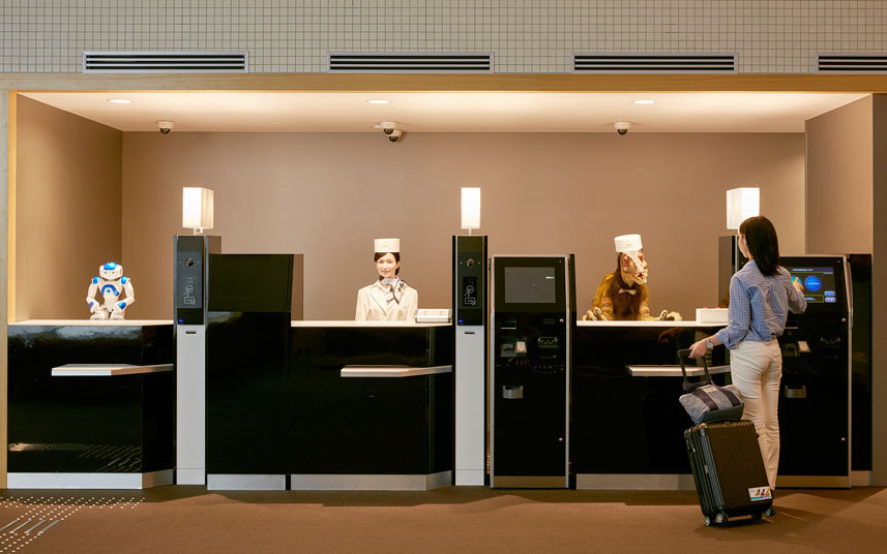
\includegraphics[width=0.75\linewidth]{images/roboter_rezeption_nagasaki.png}
\end{center}

\subsection{Der Mensch als „Bug“ des Systems}

Ein besonders wichtiges Beispiel
für die Ambivalenz menschlicher Fehlbarkeit
ist Stanislaw Petrow.

Petrow war Oberstleutnant
der sowjetischen Luftverteidigungsstreitkräfte.

Im Jahr 1983 meldete ein sowjetisches Frühwarnsystem
einen angeblichen Raketenangriff.

Petrow glaubte dem System jedoch nicht.

Seine Entscheidung verhinderte möglicherweise
eine militärische Katastrophe.

Dieses Beispiel zeigt,
dass menschliche Abweichung
nicht nur als Fehler verstanden werden kann.

Gerade weil Menschen zweifeln,
Kontext berücksichtigen
und technische Signale interpretieren können,
können sie in bestimmten Situationen
entscheidend sein.

Der Mensch ist also nicht einfach ein „Bug“ des Systems.

Er kann auch notwendig sein,
um Maschinenfehler zu erkennen
und technische Systeme kritisch zu überprüfen.

\subsection{Zur Geschichte der Künstlichen Intelligenz}

Die Geschichte der Künstlichen Intelligenz
weist einige historiographische Besonderheiten auf.

Sie lässt sich einerseits relativ schnell erzählen,
weil es vergleichsweise wenige grosse Entwicklungsschritte gibt.

Andererseits ist sie stark gegenwartsbezogen,
weil KI erst seit einigen Jahren
eine breite gesellschaftliche Relevanz besitzt.

Die Geschichte der KI lässt sich grob
in drei Phasen einteilen:

\begin{itemize}
\item Formalisierung von Denken und Denkprozessen
\item KI-Winter in den 1980er und 1990er Jahren
\item datengetriebene Modelle seit den 1980er Jahren mit Durchbruch in den 2010er Jahren
\end{itemize}

In der ersten Phase stand die Idee im Zentrum,
Denken so weit zu formalisieren,
dass es in Programmcode übersetzt werden kann.

Diese Idee kann je nach Perspektive
bis in die Antike,
in die Frühe Neuzeit
oder in die Mitte des 20. Jahrhunderts zurückverfolgt werden.

In der zweiten Phase,
dem sogenannten KI-Winter,
ging die Forschungsförderung zurück,
weil die Ergebnisse hinter den Erwartungen zurückblieben.

In der dritten Phase wurden Modelle
mit möglichst vielen Daten trainiert.

Diese datengetriebene Entwicklung
führte ab den 2010er Jahren
zu wichtigen Durchbrüchen.

\subsection{KI und die Frage nach Intelligenz}

Die Geschichte der KI ist eng verbunden
mit der Frage,
was Intelligenz eigentlich bedeutet.

Wer über KI nachdenkt,
denkt immer auch darüber nach,
was Menschen ausmacht.

Künstliche Intelligenz zwingt dazu,
menschliche Fähigkeiten zu definieren,
zu formalisieren
und mit maschinellen Leistungen zu vergleichen.

Dabei wird häufig spekuliert,
welche menschlichen Fähigkeiten
Maschinen übernehmen könnten.

Diese Spekulation betrifft nicht nur Rechnen
oder logisches Problemlösen,
sondern auch Sprache,
Wahrnehmung,
Entscheidung,
Kreativität
und soziale Interaktion.

Gerade deshalb ist KI nicht nur ein technisches,
sondern auch ein philosophisches,
soziales und politisches Thema.

\subsection{Schach als Leitmedium der KI-Forschung}

Ein wichtiges Beispiel in der Geschichte der KI
ist der Schachcomputer.

Schach wurde lange als Leitmedium
der KI-Forschung betrachtet.

Der Grund dafür liegt in der Struktur des Spiels.

Schach besitzt klare Regeln
und eine begrenzte Anzahl möglicher Züge,
auch wenn diese Anzahl sehr gross ist.

Damit eignet sich Schach gut,
um maschinelles Problemlösen zu testen.

Gleichzeitig zeigt das Beispiel aber auch
eine Einschränkung.

Schach bildet nur eine sehr enge Form von Intelligenz ab.

Es geht um logisches Problemlösen
in einem klar abgegrenzten Regelraum.

Andere Dimensionen menschlicher Intelligenz
spielen dabei keine Rolle.

Dazu gehören:

\begin{itemize}
\item Sprache
\item soziale Beziehungen
\item Widerspruch
\item Körperlichkeit
\item Emotion
\item Politik
\end{itemize}

Der Sieg von Deep Blue gegen Garri Kasparov 1997
wurde deshalb als Zeichen maschineller Überlegenheit verstanden.

Er zeigte aber vor allem,
dass Maschinen in klar definierten Aufgabenräumen
sehr leistungsfähig sein können.

\begin{center}
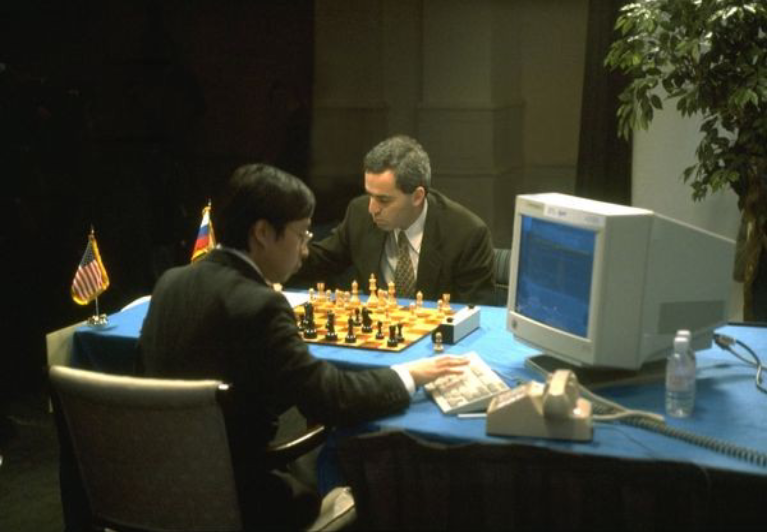
\includegraphics[width=0.75\linewidth]{images/kasparov_deep_blue.png}
\end{center}

\subsection{Fehlbarkeit von Mensch und Maschine}

Unter den Bedingungen des Schachs
erscheint der Mensch spätestens seit Deep Blue
auch im Bereich der Intelligenz unterlegen.

Wenn man jedoch Sprachmodelle wie ChatGPT betrachtet,
verschiebt sich diese Einschätzung.

Sprachmodelle arbeiten nicht in einem klar abgegrenzten Regelraum
wie dem Schachspiel.

Sie bewegen sich in offenen,
mehrdeutigen und sozialen Bedeutungsräumen.

Dadurch wird auch die Fehlerhaftigkeit der Maschine
wieder sichtbar.

Maschinen können falsche Informationen erzeugen,
Zusammenhänge missverstehen
oder scheinbar überzeugende Antworten geben,
die sachlich nicht stimmen.

Die Fehlbarkeit liegt daher nicht nur beim Menschen.

Auch Maschinen machen Fehler.

Entscheidend ist,
dass diese Fehler anders entstehen
und oft schwieriger zu erkennen sind.

\subsection{Digitale Technik und Wartung}

Von der Industrialisierung bis zur Mitte des 20. Jahrhunderts
wurden Maschinen häufig als Mittel verstanden,
um fehlbare Menschen zu entlasten,
zu unterstützen oder zu ersetzen.

Ab den 1960er Jahren,
besonders mit der Digitaltechnik,
veränderte sich dieses Verhältnis.

Der Mensch wurde zunehmend notwendig,
um komplexe Maschinen und Systeme
funktional am Laufen zu halten.

Fehlersuche,
Wartung,
Kontrolle und Anpassung
wurden zentrale Aufgaben.

Gleichzeitig wurden technische Systeme immer komplexer.

Menschen überblickten ihre Systeme
immer weniger vollständig.

Dadurch wurde die Fehlersuche
aufwändig,
ineffizient
und selbst wieder zu einem Problem,
das technisch gelöst werden sollte.

Technik erzeugt also nicht nur Entlastung,
sondern auch neue Arbeit.

\subsection{KI und die Neuordnung des Mensch-Maschinen-Verhältnisses}

Mit KI wird das Mensch-Maschinen-Verhältnis
noch einmal neu geordnet.

Die Frage lautet nicht mehr nur,
ob Maschinen Menschen ersetzen können.

Vielmehr geht es darum,
wer in komplexen Systemen
welche Rolle übernimmt.

KI-Systeme können menschliche Arbeit unterstützen,
aber auch menschliche Fehler reproduzieren.

Sie können Entscheidungen vorbereiten,
aber auch Verantwortung verschieben.

Wichtige Fragen sind daher:

\begin{itemize}
\item Wer kontrolliert KI-Systeme?
\item Wer erkennt Maschinenfehler?
\item Wer trägt Verantwortung für technische Entscheidungen?
\item Reproduziert KI menschliche Vorurteile?
\item Wann ist menschliches Eingreifen notwendig?
\end{itemize}

KI zeigt damit besonders deutlich,
dass die Grenze zwischen menschlicher
und maschineller Fehlbarkeit
nicht eindeutig ist.

Menschen machen Fehler.

Maschinen machen Fehler.

Und KI kann menschliche Fehler
in technische Systeme einschreiben,
verstärken und automatisieren.

\subsection{Zentrale Erkenntnisse}

Die Vorlesung zeigt,
dass die Geschichte der KI
nicht nur als Geschichte technischer Innovationen
verstanden werden kann.

Sie ist Teil einer längeren Technikgeschichte,
in der Menschen Maschinen entwickeln,
um Probleme zu lösen,
Arbeit zu erleichtern,
Effizienz zu steigern
und eigene Grenzen zu überwinden.

Zentrale Erkenntnisse sind:

\begin{itemize}
\item Technikentwicklung beruht auf verschiedenen Faktoren wie Problemlösung, Wachstum, Wissenschaft, Staat, Militär und sozialer Aushandlung.
\item Technik ist nicht neutral, sondern enthält gesellschaftliche Normen, Interessen und Menschenbilder.
\item Der Mensch wird in der Technikgeschichte häufig als fehlerhaftes Wesen beschrieben.
\item Maschinen erscheinen oft als überlegen, weil sie als rational, ausdauernd und neutral gelten.
\item Diese Vorstellung übersieht, dass auch Maschinen fehlerhaft sind.
\item KI verschiebt die Frage nach Fehlbarkeit, Verantwortung und Kontrolle neu.
\end{itemize}

Die zentrale These lautet:

KI verändert das Mensch-Maschinen-Verhältnis nicht,
weil Maschinen plötzlich vollkommen fehlerfrei wären.

Sie verändert es,
weil menschliche und maschinelle Fehlbarkeit
enger miteinander verbunden werden.

Die Geschichte der KI ist daher immer auch
eine Geschichte darüber,
wie Menschen sich selbst,
ihre Schwächen
und ihre Verantwortung
im Spiegel der Maschine verstehen.

        \section{Objektivität und technische Vermittlung: Technisierung der Wissenschaften}

\subsection{Einführung: Wissenschaft, Technik und Objektivität}

Die Vorlesung untersucht,
wie sich wissenschaftliche Objektivität historisch verändert hat
und welche Rolle technische Instrumente
in der modernen Wissensproduktion spielen.

Im Zentrum steht die Frage,
wie wissenschaftliche Erkenntnis entsteht,
wenn Beobachtung,
Messung und Darstellung zunehmend
durch technische Verfahren vermittelt werden.

Wissenschaft erscheint häufig als objektiv,
weil sie sich auf Daten,
Messinstrumente,
Modelle und standardisierte Verfahren stützt.

Die Vorlesung zeigt jedoch,
dass auch diese Formen von Objektivität
eine Geschichte haben.

Zentrale Leitfragen:

\begin{itemize}
\item Was bedeutet wissenschaftliche Objektivität?
\item Wie verändern technische Instrumente wissenschaftliche Erkenntnis?
\item Warum sind Daten nicht einfach selbsterklärend?
\item Wie entsteht Vertrauen in wissenschaftliche Verfahren?
\item Weshalb kann wissenschaftliche Unsicherheit politisch instrumentalisiert werden?
\end{itemize}

Objektivität ist daher nicht einfach gegeben,
sondern entsteht durch historische,
technische,
soziale und institutionelle Praktiken.

\subsection{Quellenkritik und historisches Argumentieren}

Zu Beginn der Sitzung wurde nochmals
auf die Quellenkritik zu Kasparov und Deep Blue eingegangen.

Für die Prüfung ist wichtig,
dass Quellenkritik als Fliesstext geschrieben wird.

Es sollen also ganze Sätze formuliert werden,
nicht nur Stichworte.

Dabei müssen nicht alle möglichen Fragen beantwortet werden.

Entscheidend sind diejenigen Fragen,
die für Analyse und Interpretation der Quelle relevant sind.

Eine Quelleninterpretation soll sich nicht primär
an der persönlichen Meinung
der schreibenden Person orientieren.

Stattdessen geht es darum,
auf Grundlage der Quelle zu argumentieren.

Die zentrale Frage lautet also nicht:

Was denke ich selbst über Mensch und Maschine?

Sondern:

Wie lässt sich historisch erklären,
weshalb eine Quelle bestimmte Vorstellungen
über das Mensch-Maschinen-Verhältnis ausdrückt?

Wichtig ist daher eine stringente Argumentation.

Die eigene Interpretation muss begründet werden,
indem gezeigt wird,
wie sie aus der Quelle abgeleitet wird.

\subsection{Kasparov vs. Deep Blue als Beispiel der Quellenkritik}

Am Beispiel eines Zeit-Artikels
zu Kasparov und Deep Blue wurde gezeigt,
wie eine solche Quellenkritik aussehen kann.

Die Zeit ist eine liberale deutsche Wochenzeitung.

Der Artikel richtete sich nicht an Fachleute,
sondern an eine breite Leserschaft.

Technische Vorkenntnisse wurden nicht vorausgesetzt.

Der Artikel entstand zwischen dem ersten
und dem zweiten Aufeinandertreffen
von Garri Kasparov und Deep Blue.

Zu diesem Zeitpunkt war noch nicht bekannt,
dass Deep Blue Kasparov 1997 schlagen würde.

Der Artikel kündigte das zweite Spiel an
und blickte zugleich auf das erste zurück.

Auffällig ist,
dass Deep Blue einerseits personifiziert wird.

Es wird etwa von seinem „zweiten Leben“
oder von einer Software mit mehr „Gefühl“ gesprochen.

Andererseits wird seine technische Besonderheit
teilweise relativiert.

Es wird darauf hingewiesen,
dass es bereits andere Schachcomputer gebe,
die anders funktionierten
und in gewisser Weise moderner seien.

Der Artikel stellt also keine einfache Überlegenheit
der Maschine gegenüber dem Menschen fest.

Vielmehr erscheint Deep Blue
als Übergangsfigur einer älteren KI-Entwicklung,
während sich die KI-Forschung Ende der 1990er Jahre
bereits in andere Richtungen bewegte.

\subsection{„A Frank Statement to Cigarette Smokers“, 1954}

Ein zentrales Beispiel der Vorlesung
ist die Medienkampagne der US-amerikanischen Tabakindustrie
aus dem Jahr 1954.

Unter dem Titel
„A Frank Statement to Cigarette Smokers“
wandte sich die Tabakindustrie
an die Öffentlichkeit.

Hintergrund war,
dass wissenschaftliche Studien
seit dem frühen 20. Jahrhundert
auf die gesundheitlichen Gefahren des Rauchens hinwiesen.

Ab den 1950er Jahren nahm die Zahl der Todesfälle zu,
die mit Lungenerkrankungen in Verbindung gebracht wurden.

In den USA und anderen westlichen Staaten
begann man deshalb,
politische Regulierungen auszuarbeiten.

Dagegen wehrte sich die Tabakindustrie.

Die Kampagne stellte die wissenschaftlichen Arbeiten
nicht offen als unwissenschaftlich dar.

Stattdessen wurde behauptet,
dass die Beweislage noch nicht eindeutig genug sei.

Die Tabakindustrie argumentierte unter anderem:

\begin{itemize}
\item Medizinische Forschungen hätten auf viele mögliche Ursachen von Lungenkrebs hingewiesen.
\item Unter Fachleuten herrsche keine Einigkeit über die eigentliche Ursache.
\item Es gebe keinen Beweis dafür, dass Zigarettenrauchen eine Ursache sei.
\item Statistiken könnten ebenso gut andere Aspekte des modernen Lebens betreffen.
\end{itemize}

Damit wurde nicht die Wissenschaft als solche angegriffen.

Vielmehr wurden Unsicherheiten der wissenschaftlichen Beweisführung betont.

Ziel war es,
Zweifel zu säen.

\begin{center}
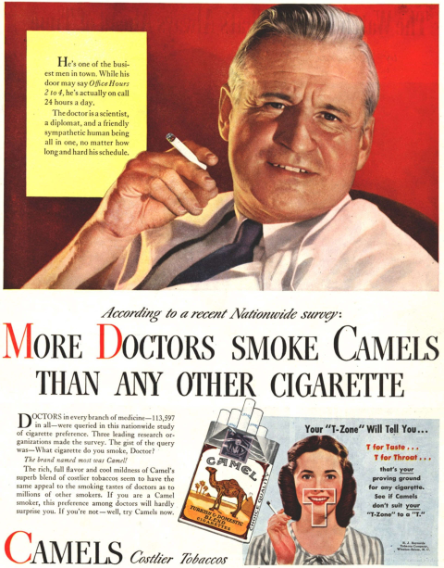
\includegraphics[width=0.65\linewidth]{images/frank_statement_cigarette_smokers.png}
\end{center}

\subsection{Strategische Unsicherheit und die Tabakindustrie}

In den folgenden Jahren
wurden ähnliche Kampagnen wiederholt durchgeführt.

Die Tabakindustrie stellte sich dabei nicht
grundsätzlich gegen Wissenschaft.

Sie bewegte sich vielmehr innerhalb
einer wissenschaftlichen Logik.

Behauptet wurde,
dass es noch keinen stichhaltigen Beweis
für den Zusammenhang zwischen Rauchen
und Lungenerkrankungen gebe.

Gleichzeitig investierte die Tabakindustrie
selbst in wissenschaftliche Forschung.

Diese Forschung sollte zeigen,
dass ein Zusammenhang nicht eindeutig bewiesen werden könne.

In den 1970er Jahren beauftragte
die R.J. Reynolds Tobacco Company
beispielsweise den renommierten Physiker Fred Seitz.

Seitz war ehemaliger Präsident
der US National Academy of Sciences.

Er trat nicht als Wissenschaftsskeptiker auf.

Stattdessen erklärte er,
warum die vorhandenen Forschungsergebnisse
noch nicht ausreichten,
um klare Aussagen zu machen
oder politische Regulierungen zu begründen.

Daran zeigt sich eine wichtige Strategie:

Wissenschaftliche Unsicherheit wurde nicht beseitigt,
sondern gezielt produziert und verstärkt.

\subsection{Merchants of Doubt}

Eine ähnliche Strategie lässt sich
in den Debatten um das Ozonloch beobachten.

In den 1970er und 1980er Jahren
waren Wissenschaft und Politik
zunächst vorsichtig mit ihren Interpretationen.

Die Atmosphärenforschung war komplex,
die Datenlage begrenzt
und viele Fragen waren offen.

Diese Form von Unsicherheit
gehört grundsätzlich zur normalen wissenschaftlichen Praxis.

Sie ist sogar wichtig
für wissenschaftliche Glaubwürdigkeit,
weil Wissenschaft ihre eigenen Grenzen
und Unsicherheiten reflektieren muss.

Gleichzeitig wurden Umweltpolitik
und Regulierung ab den 1970er Jahren
zunehmend denkbar.

Deshalb traten Industrievertreter
und verbündete Wissenschaftlerinnen und Wissenschaftler
auf den Plan.

Besonders wichtig war dabei DuPont,
ein grosser Produzent von Fluorchlorkohlenwasserstoffen.

Diese Stoffe wurden unter anderem
als Treibgase,
Kältemittel und Lösemittel verwendet.

Industrievertreter zweifelten Messverfahren,
Modelle und Interpretationen an.

Sie forderten,
dass vor politischen Regulierungen
mehr Beweise geliefert werden müssten.

Auch hier wurde wissenschaftliche Unsicherheit
politisch genutzt.

\subsection{Die Entdeckung des Ozonlochs}

Im Jahr 1985 stellten britische Forscherinnen und Forscher
einen drastischen Rückgang der Ozonkonzentration
über der Antarktis fest.

Sie konnten den Zusammenhang
zwischen bestimmten Emissionen
und dem Ozonabbau nachweisen.

Diese Entdeckung führte später
zu weltweiten politischen Massnahmen.

Die Zweifel am Bestehen des Ozonlochs
verschwanden jedoch nicht sofort.

Trotzdem wurden auf politischer Ebene
verschiedene Massnahmen zur Reduktion
ozonschädigender Stoffe ergriffen.

Das Beispiel zeigt,
dass wissenschaftliche Erkenntnis
nicht automatisch und unmittelbar
zu politischem Handeln führt.

Zwischen Messung,
Interpretation,
Anerkennung und Regulierung
liegen gesellschaftliche und politische Aushandlungsprozesse.

\begin{center}
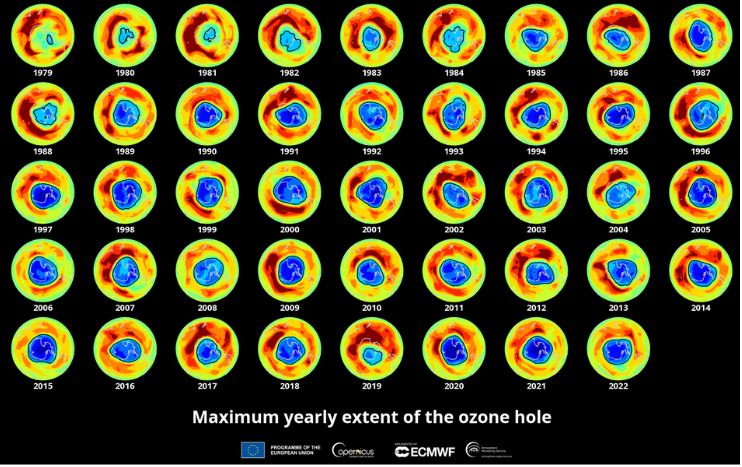
\includegraphics[width=0.75\linewidth]{images/ozonloch_1985.png}
\end{center}

\subsection{Objektivität und technische Vermittlung}

Besonders interessant ist,
dass die Satellitendaten,
mit denen das Ozonloch nachgewiesen werden konnte,
bereits früher vorhanden waren.

Sie wurden jedoch zunächst
als Ausreisser interpretiert
und aus den Berechnungen ausgeschlossen.

Die Werte erschienen zu extrem
und passten nicht in das bestehende Wissenssystem.

Sie wurden deshalb als Messfehler behandelt.

Das bedeutet:

Auch diejenigen,
die einen begründeten Verdacht
für die Existenz des Ozonlochs hatten,
vertrauten ihren Daten nicht blind.

Daten sprechen nicht einfach für sich selbst.

Sie müssen erhoben,
gefiltert,
korrigiert,
modelliert
und interpretiert werden.

Technische Messinstrumente liefern daher
keine unmittelbare Wahrheit.

Sie vermitteln zwischen Welt und Darstellung.

\subsection{Daten, Modelle und Interpretation}

Die Daten zum Ozonloch wurden nicht abgelehnt,
weil sie unwissenschaftlich gewesen wären.

Sie passten nicht
zu den vorhandenen Modellen
und Wissenssystemen.

Gerade bei komplexen Messinstrumenten
wie Satelliten ist dies besonders wichtig.

Satellitendaten brauchen Korrekturen,
Filter und Modelle.

Erst dadurch werden sie
zu wissenschaftlich nutzbaren Daten.

Daten sind also interpretationsbedürftig.

Wie sie erhoben,
bearbeitet
und als zuverlässig eingestuft werden,
ist nicht einfach gegeben.

Eine lückenlose Beweisführung
beruht daher immer auch
auf begründeten Annahmen.

Damit stellt sich die Frage,
was dies für den Objektivitätsanspruch
der Wissenschaft bedeutet.

\subsection{Die Geschichte des Objektivitätsanspruchs}

Die Vorlesung zeigt,
dass auch wissenschaftliche Objektivität
eine Geschichte hat.

Vor dem 19. Jahrhundert
stand häufig das Ideal der Naturwahrheit im Zentrum.

Gesucht wurde nicht unbedingt
die exakte Wiedergabe jedes einzelnen Details.

Stattdessen ging es darum,
das Wesentliche,
Typische,
Regelhafte oder Ideale der Natur zu erfassen.

Das Zufällige wurde zugunsten
eines Ideals korrigiert.

Ziel war es,
ein „inneres Gesetz“ der Natur zu erkennen.

Erkenntnis entstand durch geschultes Urteil.

Erfahrung,
Bildung
und Urteilskraft der Forschenden
galten als entscheidend.

Subjektivität wurde hier nicht als Fehler angesehen,
sondern als Kompetenz.

\subsection{Mit geschultem Urteil zur Naturwahrheit}

Beispiele für diese Form der Naturwahrheit
sind Carl von Linnés Taxonomie
und Robert Hookes \emph{Micrographia}.

Linnés Natursystem von 1758
ordnete Lebewesen nach systematischen Kriterien.

Dabei ging es darum,
Regelmässigkeiten und Ordnungen
in der Natur sichtbar zu machen.

Robert Hookes \emph{Micrographia} von 1665
zeigte mikroskopische Darstellungen,
etwa die berühmte Zeichnung eines Flohs.

Solche Darstellungen waren nicht einfach
mechanische Abbilder.

Sie beruhten auf Beobachtung,
Auswahl,
Zeichnung
und Urteil.

Wissenschaftliche Darstellung bedeutete,
das Gesehene so aufzubereiten,
dass sein wesentliches Merkmal
erkennbar wurde.

\begin{center}
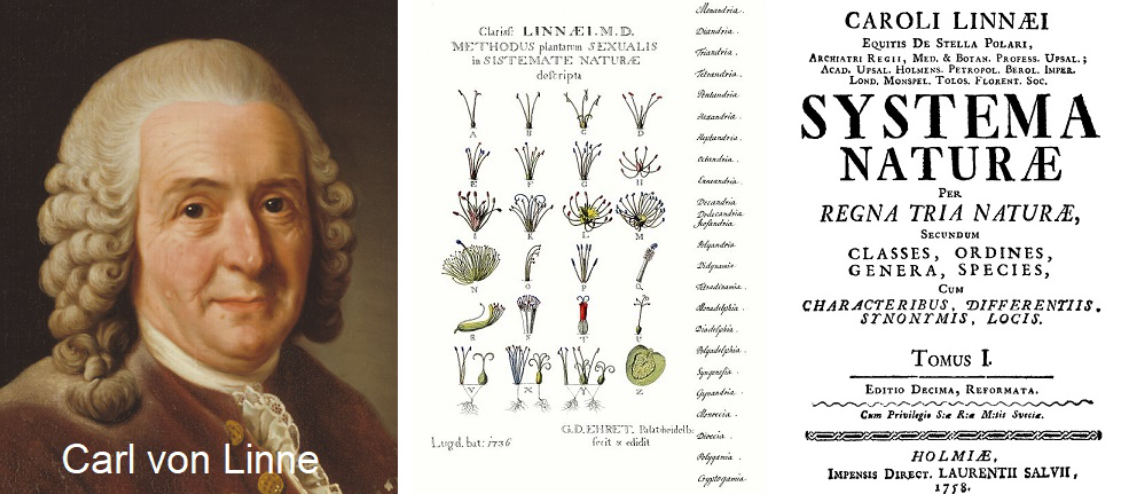
\includegraphics[width=0.9\linewidth]{images/naturwahrheit_linne_hooke.png}
\end{center}

\subsection{Mechanische Objektivität}

Seit dem Ende des 19. Jahrhunderts
veränderte sich dieses Ideal.

Subjektivität wurde zunehmend
als unwissenschaftlich betrachtet.

Forschende sollten sich
so weit wie möglich zurücknehmen.

Wissenschaftliche Experimente wurden wichtiger,
und damit auch technische Instrumente.

Besonders neue Bild-
und Aufzeichnungsverfahren
galten als Mittel der Objektivierung.

Dazu gehörten:

\begin{itemize}
\item Photographie
\item Kymographen
\item automatische Aufzeichnungsgeräte
\item Bewegungsstudien
\item Messapparate
\end{itemize}

Individuelles Urteil
und subjektive Wahrnehmung
wurden durch technische Instrumente
in Frage gestellt.

Technik sollte das „Sehen“ übernehmen
und möglichst rohe Daten produzieren.

Statt idealisierender Darstellungen
sollten technische Aufzeichnungen
die Natur scheinbar unmittelbar festhalten.

\subsection{Technische Aufzeichnung und Objektivierung}

Beispiele für mechanische Objektivität
sind die Bewegungsstudien
von Eadweard Muybridge aus dem Jahr 1887
und die automatische Aufzeichnung
eines Bebens in Wien 1908.

Muybridges Fotografien zerlegten Bewegungen
in einzelne Bildsequenzen.

Dadurch konnten Bewegungsabläufe
technisch sichtbar gemacht werden,
die dem menschlichen Auge
in dieser Form nicht zugänglich waren.

Auch die automatische Aufzeichnung
eines Bebens zeigt,
wie technische Instrumente
als objektive Zeugen verstanden wurden.

Nicht mehr das geschulte Auge
der Forschenden sollte entscheiden,
sondern die Maschine sollte registrieren.

Damit entstand ein neues Ideal:

Objektiv ist,
was möglichst unabhängig
vom subjektiven Urteil
der Forschenden aufgezeichnet wird.

\begin{center}
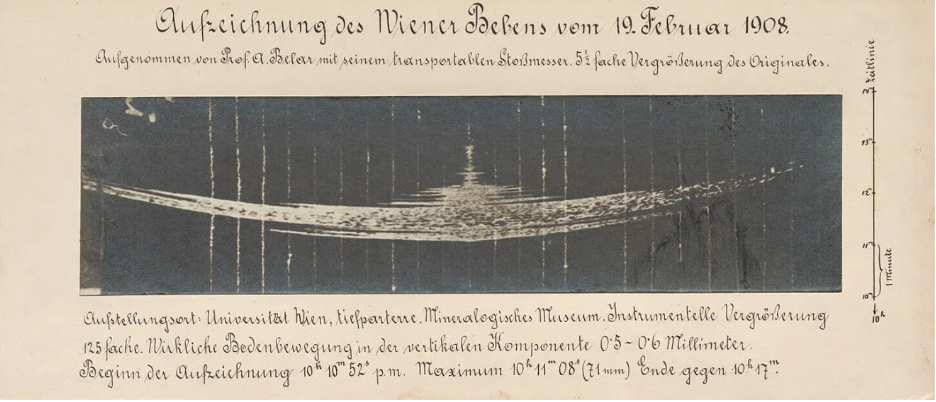
\includegraphics[width=0.9\linewidth]{images/mechanische_objektivitaet.png}
\end{center}

\subsection{Strukturelle Objektivität}

Im Verlauf des 20. Jahrhunderts
entwickelte sich zusätzlich
das Ideal der strukturellen Objektivität.

Diese löste die mechanische Objektivität
nicht einfach ab,
sondern entstand parallel dazu.

Sie erweiterte,
was als objektive wissenschaftliche Praxis galt.

In vielen Bereichen
wurde reines Aufzeichnen unpraktisch.

Besonders in der Atomphysik,
Quantenmechanik
oder Klimaforschung
sind die untersuchten Gegenstände
nicht mehr direkt beobachtbar.

Zudem erzeugen technische Messsysteme
riesige Datenmengen.

Deshalb wurden statistische Modelle,
mathematische Formeln,
formale Strukturen
und Simulationen zentral.

Forschende sollen sich dabei
in Regeln und Verfahren
wissenschaftlicher Praxis einfügen.

Sie treten hinter formale Systeme zurück,
bleiben aber dennoch Teil der Wissensproduktion.

\subsection{Modelle, Simulationen und wissenschaftliche Praxis}

Strukturelle Objektivität bedeutet nicht,
dass Forschende verschwinden.

Sie entscheiden weiterhin,
welche Modelle,
Daten,
Verfahren
und Annahmen verwendet werden.

Diese Entscheidungen müssen jedoch
innerhalb bestehender Wissenssysteme
begründet werden.

Objektivität entsteht also
durch nachvollziehbare Verfahren,
Standardisierung,
Dokumentation
und methodische Begründung.

Ein Beispiel dafür sind Klimamodelle.

Sie beruhen nicht auf einfacher Beobachtung,
sondern auf komplexen Simulationen.

Die in der Vorlesung gezeigte Simulation
mit historischen CO2-Emissionen
und einem angenommenen Emissionsstopp
am 1. Januar 2021
zeigt,
wie wissenschaftliche Erkenntnis
durch formale Modelle erzeugt wird.

Solche Modelle sind nicht einfach Bilder der Wirklichkeit.

Sie sind strukturierte,
technisch vermittelte Darstellungen,
die auf Annahmen,
Daten und Berechnungen beruhen.

\begin{center}
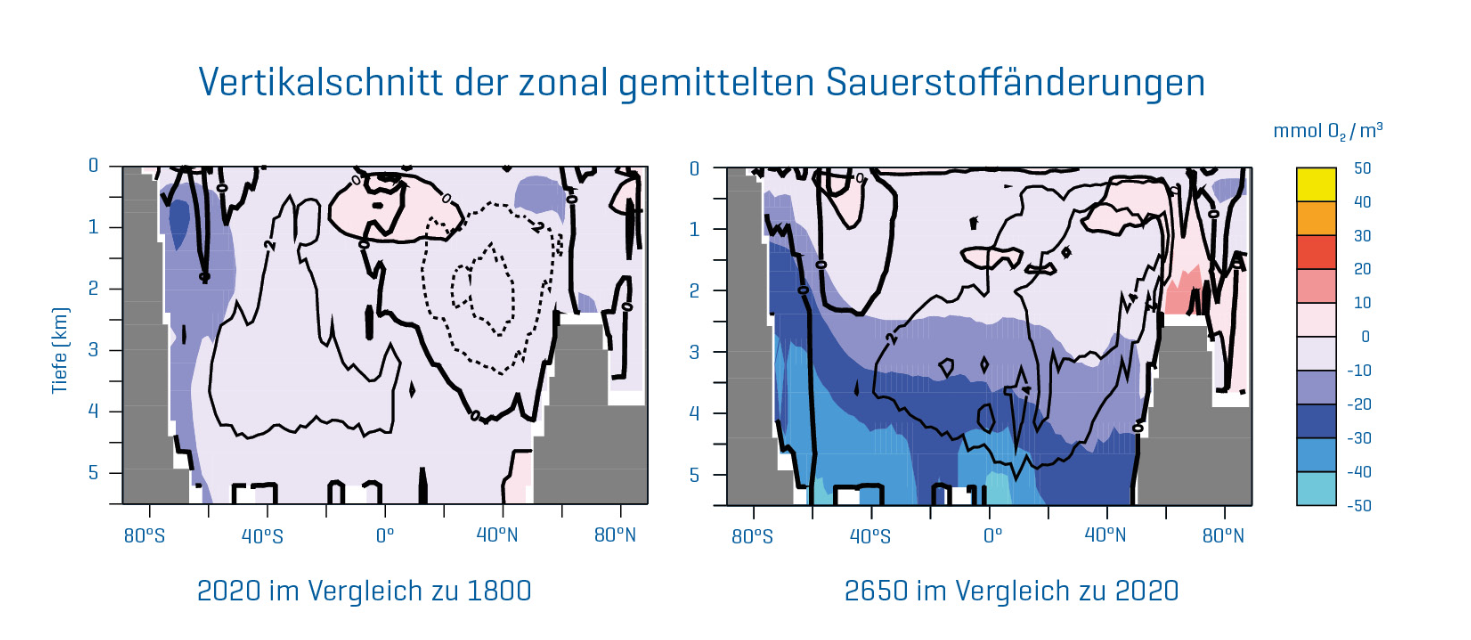
\includegraphics[width=0.9\linewidth]{images/strukturelle_objektivitaet_klimamodell.png}
\end{center}

\subsection{Glaubwürdigkeit und Technik}

Wie technische Instrumente
in der wissenschaftlichen Praxis eingesetzt werden,
stand historisch nicht einfach fest.

Innerhalb wissenschaftlicher Disziplinen
mussten sich stabile Praktiken herausbilden.

Diese Praktiken legten fest,
welche technischen Verfahren
als zuverlässig gelten konnten.

Dafür waren besonders wichtig:

\begin{itemize}
\item Standardisierung
\item Dokumentation
\item methodische Begründung
\item Wiederholbarkeit
\item disziplinäre Aushandlung
\end{itemize}

Vertrauen in technische Verfahren
entsteht also nicht automatisch.

Es ist Ergebnis historischer Aushandlungsprozesse.

Ein Messinstrument ist nicht allein deshalb glaubwürdig,
weil es technisch ist.

Es wird glaubwürdig,
wenn seine Anwendung stabilisiert,
dokumentiert
und innerhalb einer wissenschaftlichen Gemeinschaft
anerkannt wird.

\subsection{Angreifbarkeit wissenschaftlicher Objektivität}

Die Stabilisierung wissenschaftlicher Praktiken
ist nie völlig abgeschlossen.

Zudem ist sie von aussen
oft schwer nachvollziehbar.

Für Nicht-Fachleute ist es schwierig zu beurteilen,
ob ein Verfahren richtig oder falsch angewendet wurde
und welche epistemische Autorität es besitzt.

Das macht wissenschaftliche Objektivität
prinzipiell angreifbar.

Technische Vermittlung erzeugt immer eine Differenz
zwischen Welt und Darstellung,
zwischen Messung und Interpretation.

Diese Differenz kann in Zweifel gezogen werden.

Genau hier setzen Strategien
strategischer Unsicherheit an.

Die Tabakindustrie
und die Skeptiker des Ozonlochs
griffen nicht unbedingt Wissenschaft als Ganzes an.

Sie nutzten vielmehr die Tatsache,
dass wissenschaftliche Erkenntnis
immer technisch vermittelt,
modelliert
und begründungsbedürftig ist.

\subsection{Politische Dimension moderner Wissensproduktion}

Strategische Unsicherheit verweist
auf die politische Dimension
moderner und postmoderner Wissensproduktion.

Wissenschaftliche Unsicherheit
ist an sich nichts Unwissenschaftliches.

Sie gehört zur Wissenschaft.

Problematisch wird sie,
wenn Unsicherheit gezielt erzeugt,
übertrieben
oder politisch instrumentalisiert wird,
um Regulierung zu verhindern.

Die Beispiele der Tabakindustrie
und der Ozonloch-Debatte zeigen,
dass wissenschaftliche Objektivität
in politischen Konflikten
eine zentrale Rolle spielt.

Wer bestimmen kann,
was als bewiesen,
unsicher
oder noch nicht ausreichend geklärt gilt,
kann politische Entscheidungen beeinflussen.

Technik,
Wissenschaft
und Politik sind daher eng miteinander verbunden.

\subsection{Zentrale Erkenntnisse}

Die Vorlesung zeigt,
dass wissenschaftliche Objektivität
nicht zeitlos und unveränderlich ist.

Sie hat sich historisch gewandelt
und ist eng mit technischen Verfahren
der Beobachtung,
Messung,
Aufzeichnung
und Modellierung verbunden.

Zentrale Erkenntnisse sind:

\begin{itemize}
\item Objektivität ist eine historische wissenschaftliche Tugend.
\item Vor dem 19. Jahrhundert galt geschultes Urteil als zentrale wissenschaftliche Kompetenz.
\item Seit dem späten 19. Jahrhundert wurde mechanische Objektivität wichtiger.
\item Technische Instrumente sollten subjektives Urteil zurückdrängen.
\item Im 20. Jahrhundert gewannen Modelle, Simulationen und formale Verfahren an Bedeutung.
\item Daten sind nicht selbsterklärend, sondern müssen interpretiert und in Wissenssysteme eingeordnet werden.
\item Wissenschaftliche Unsicherheit kann politisch instrumentalisiert werden.
\end{itemize}

Die zentrale These lautet:

Technische Vermittlung macht Wissenschaft nicht weniger objektiv.

Sie zeigt aber,
dass Objektivität nicht einfach aus Daten entsteht.

Objektivität beruht auf Verfahren,
Instrumenten,
Modellen,
Standards,
Dokumentation
und begründeten Annahmen.

Gerade deshalb ist Wissenschaft glaubwürdig,
aber zugleich auch angreifbar.

        \section{Umweltkatastrophe und Umweltbewusstsein}

\subsection{Einführung: Umwelt als technikgeschichtliches Problem}

Die Vorlesung untersucht,
wie Umweltkatastrophen und Umweltbewusstsein
im Verlauf des 20. Jahrhunderts
zu zentralen Themen moderner Technikgeschichte wurden.

Im Zentrum steht die Frage,
wie technische,
industrielle und wirtschaftliche Entwicklungen
neue Risiken hervorbrachten
und wie diese Risiken gesellschaftlich,
politisch und wissenschaftlich wahrgenommen wurden.

Umweltprobleme erscheinen dabei nicht nur
als Folgen einzelner Unfälle.

Sie entstehen auch durch langfristige,
schleichende Prozesse,
die mit moderner Produktion,
Konsum,
Energieversorgung
und globalen Stoffkreisläufen verbunden sind.

Zentrale Leitfragen:

\begin{itemize}
\item Wie entstehen technische Umweltkatastrophen?
\item Was unterscheidet plötzliche Katastrophen von schleichenden Krisen?
\item Warum wird Umwelt erst im 20. Jahrhundert zu einem gesellschaftspolitischen Problem?
\item Welche Rolle spielen Wissenschaft, Medien und Protestbewegungen?
\item Welche politischen Antworten wurden auf Umweltprobleme entwickelt?
\end{itemize}

Die Geschichte des Umweltbewusstseins ist daher
nicht nur Naturgeschichte,
sondern auch Technik-,
Wissenschafts-,
Medien-,
Politik-
und Gesellschaftsgeschichte.

\subsection{Brandkatastrophe in Schweizerhalle 1986}

Ein zentrales Beispiel der Vorlesung
ist die Brandkatastrophe in Schweizerhalle.

In der Nacht vom 1. November 1986
brach in einer Lagerhalle des Chemiekonzerns Sandoz
bei Schweizerhalle nahe Muttenz
ein Grossbrand aus.

Bei den Löscharbeiten der Feuerwehr
gelangten tonnenweise Chemikalien in den Rhein.

Die Folgen waren massiv.

Der Rhein verfärbte sich zeitweise rot,
und bis weit flussabwärts kam es
zu starkem Fischsterben.

Besonders betroffen war die Aalpopulation.

Auf einer Länge von rund 400 Kilometern
starb die gesamte Aalpopulation
von etwa 150 000 Individuen.

Die Katastrophe machte sichtbar,
wie eng industrielle Produktion,
Flüsse,
Ökosysteme
und internationale Räume miteinander verbunden sind.

Ein lokaler Brand wurde dadurch
zu einem grenzüberschreitenden Umweltproblem.

\begin{center}
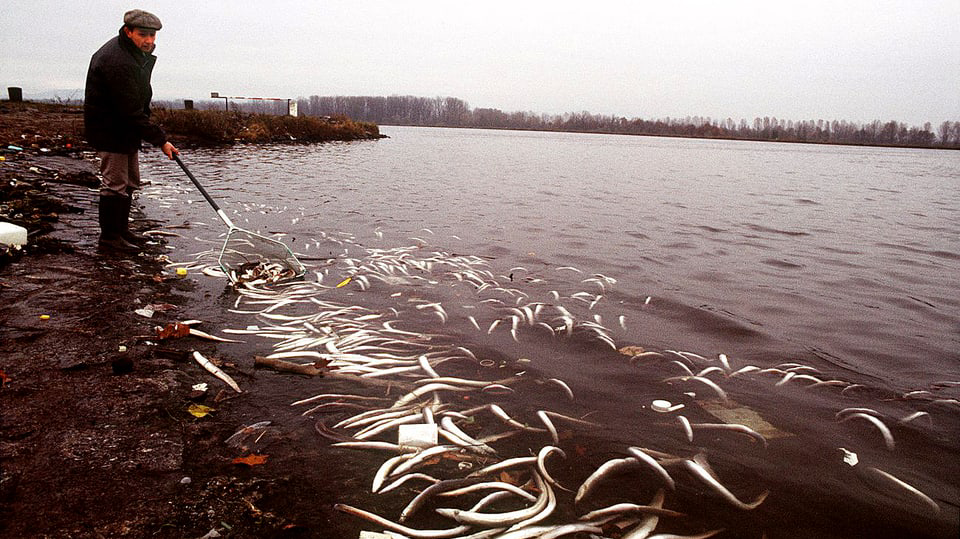
\includegraphics[width=0.8\linewidth]{images/schweizerhalle_brandkatastrophe.png}
\end{center}

\subsection{Quellenkritik zur Berichterstattung}

Die Vorlesung arbeitet am Beispiel
der Neuen Zürcher Zeitung vom 3. und 4. November 1986
auch quellenkritisch.

Untersucht werden soll,
wie über die Brandkatastrophe berichtet wurde
und welche Aspekte besonders hervorgehoben wurden.

Wichtige Fragen sind:

\begin{itemize}
\item Was berichten die Ausgaben vom 3. und 4. November?
\item Welche Aspekte der Katastrophe stehen im Vordergrund?
\item Wie unterscheiden sich die Beiträge der beiden Tage?
\item Warum wurde erst am 3. November berichtet, obwohl der Brand bereits am 1. November stattfand?
\item Welche Aspekte werden nicht erwähnt?
\end{itemize}

Diese Fragen zeigen,
dass Katastrophen nicht nur technische
oder ökologische Ereignisse sind.

Sie werden auch medial verarbeitet.

Was sichtbar wird,
welche Verantwortung benannt wird
und welche Fragen ausgeblendet bleiben,
ist Teil der gesellschaftlichen Auseinandersetzung
mit technischen Risiken.

\subsection{Ursachen und Verantwortung}

Bei Schweizerhalle stellte sich rasch
die Frage nach der Ursache des Brandes
und nach der Verantwortung.

Als mögliche Ursachen wurden
verschiedene Erklärungen diskutiert.

Dazu gehörten:

\begin{itemize}
\item Selbstentzündung durch chemische Reaktionen im Lager
\item unsachgemässe Lagerung verschiedener Produkte
\item menschliches Versagen
\item andere Zündquellen
\end{itemize}

Später wurde auch darüber berichtet,
dass möglicherweise Feuerwerkskörper
in der Halle gelagert gewesen seien.

Diese seien angeblich für die Verabschiedung
eines Kadermitarbeiters vorgesehen gewesen.

Die Frage nach der Ursache ist deshalb komplex.

Sie lässt sich nicht einfach
auf eine einzelne Person,
einen einzelnen Fehler
oder eine einzelne technische Störung reduzieren.

Vielmehr verweist sie
auf Lagerpraktiken,
Sicherheitskulturen,
Unternehmensorganisation,
chemische Prozesse
und technische Infrastrukturen.

\subsection{„Normale“ Umweltkatastrophen}

Die Brandkatastrophe von Schweizerhalle
steht in einer Reihe grosser Umwelt-
und Technikkatastrophen der 1970er und 1980er Jahre.

In den zehn Jahren vor Schweizerhalle
ereigneten sich unter anderem:

\begin{itemize}
\item 1976: Chemieunfall von Seveso in Italien
\item 1978: Öltankerunglück der Amoco Cadiz vor der Bretagne
\item 1979: Reaktorkatastrophe von Three Mile Island in den USA
\item 1984: Chemiekatastrophe von Bhopal in Indien
\item 1986: Reaktorkatastrophe von Tschernobyl in der Ukraine
\end{itemize}

Diese Ereignisse verstärkten den Eindruck,
dass moderne Grosstechnologien
nicht nur Fortschritt,
Wohlstand und Effizienz erzeugen,
sondern auch neue Formen systemischer Risiken.

Katastrophen erschienen nicht mehr
als seltene Ausnahmen,
sondern als mögliche Normalfolge
hochkomplexer technischer Systeme.

\begin{center}
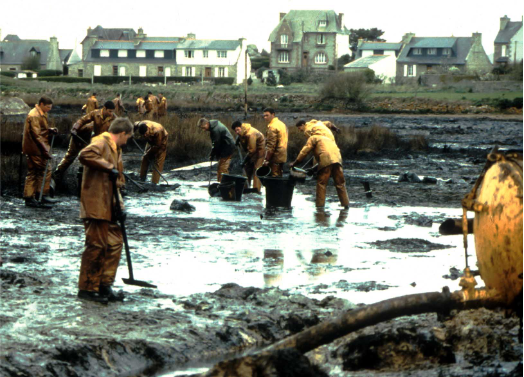
\includegraphics[width=0.75\linewidth]{images/normale_umweltkatastrophen.png}
\end{center}

\subsection{Charles Perrow und normale Katastrophen}

Der Soziologe Charles Perrow
prägte den Begriff der „normalen Katastrophen“.

Damit meinte er,
dass Katastrophen in komplexen
und eng gekoppelten technischen Systemen
nicht einfach vermeidbare Ausnahmen sind.

Moderne Grosstechnologien bestehen
aus vielen Teilsystemen,
die voneinander abhängig sind.

Wenn diese Systeme eng gekoppelt sind,
können kleine Störungen
schnell und unvorhersehbar
zu grösseren Krisen eskalieren.

Unfälle entstehen daher nicht nur
durch „menschliches Versagen“.

Sie entstehen aus dem Zusammenspiel
von Technik,
Organisation,
Kontrollsystemen,
Umweltbedingungen
und menschlichen Handlungen.

Sicherheitsmassnahmen können dabei
neue Komplexität erzeugen.

Zusätzliche Kontrollsysteme
schaffen manchmal neue Fehlerquellen.

Das bedeutet:

In komplexen technischen Systemen
können Katastrophen selbst dann entstehen,
wenn einzelne Beteiligte
nicht eindeutig falsch handeln.

\subsection{Katastrophen als gekoppelte Ereignisse}

Die Vorlesung veranschaulicht Perrows Argument
mit einer Alltagsanalogie.

Eine Person will zu einem Vorstellungsgespräch,
vergisst aber den Schlüssel im Haus.

Ein Ersatzschlüssel liegt normalerweise
unter dem Blumentopf.

Dieser wurde jedoch zuvor
dem Nachbarn gegeben,
damit er während der Ferien
die Blumen giessen kann.

Der Nachbar könnte sein Auto ausleihen,
doch dieses ist im Service.

Der Bus fällt wegen eines Streiks aus.

Taxis sind wegen des Streiks überlastet.

Am Ende verpasst die Person
das Vorstellungsgespräch.

Die Frage lautet:

Was ist die Ursache dieses „Unfalls“?

War es menschliches Versagen,
ein mechanischer Defekt,
die Umwelt
oder die Anordnung des Systems?

Diese Analogie zeigt,
dass Katastrophen häufig
durch die Verkettung vieler Faktoren entstehen.

Nicht ein einzelner Fehler ist entscheidend,
sondern die Kopplung von Ereignissen,
Notfallsystemen
und Abhängigkeiten.

\subsection{Unsichtbare und schleichende Katastrophen}

Neben plötzlichen Katastrophen
behandelt die Vorlesung auch
unsichtbare und schleichende Umweltkrisen.

Dazu gehören:

\begin{itemize}
\item saurer Regen
\item saure Böden
\item Waldsterben
\item Ozonloch
\item Erwärmung der Meere
\item Verschmutzung von Gewässern und Grundwasser
\item Mikroplastik
\item Klimaerwärmung
\item Gletscherschmelze
\end{itemize}

Solche Krisen unterscheiden sich
von plötzlichen Katastrophen.

Sie haben meist keinen klaren Anfang,
keinen einzelnen Ort
und keinen eindeutig datierbaren Moment.

Oft werden sie erst sichtbar,
wenn langfristige Schäden
bereits eingetreten sind.

Ein Beispiel ist DDT,
das bis in die 1970er Jahre
breitflächig zur Schädlingsbekämpfung eingesetzt wurde.

Die Folgen solcher Stoffe
zeigen sich häufig erst über längere Zeiträume
und über komplexe ökologische Zusammenhänge.

\begin{center}
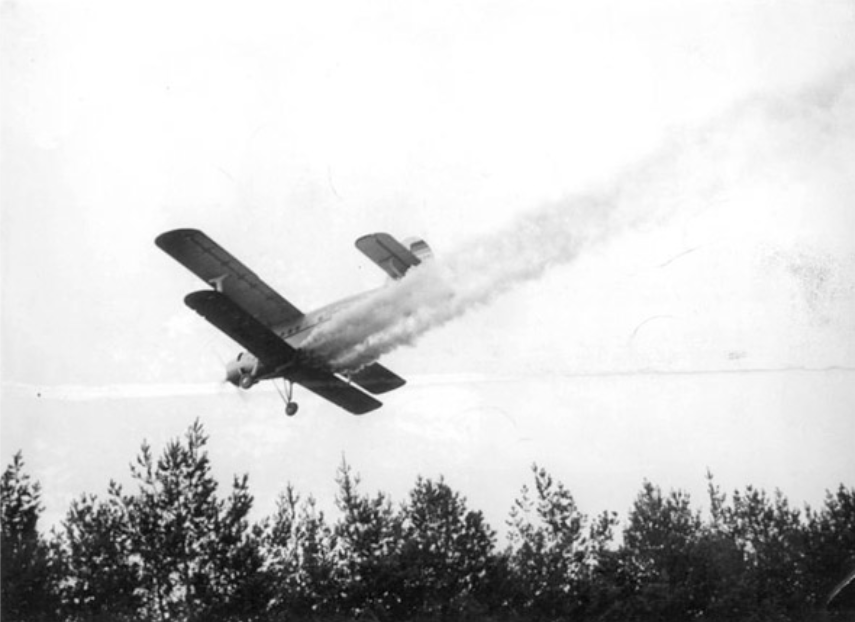
\includegraphics[width=0.75\linewidth]{images/ddt_schaedlingsbekaempfung.png}
\end{center}

\subsection{Katastrophenereignis und schleichende Krise}

Die Vorlesung unterscheidet
zwischen Katastrophenereignissen
und schleichenden Krisen.

Ein Katastrophenereignis ist meist:

\begin{itemize}
\item plötzlich
\item sichtbar
\item lokalisiert
\item datierbar
\item medial gut vermittelbar
\item mit einem Ausnahmezustand verbunden
\end{itemize}

Eine schleichende Krise ist dagegen:

\begin{itemize}
\item prozesshaft
\item häufig unsichtbar
\item diffus
\item global
\item zeitlich entgrenzt
\item schwer einzelnen Verantwortlichen zuzuordnen
\end{itemize}

Diese Unterscheidung hat wichtige Folgen.

Plötzliche Katastrophen erzeugen
mediale Aufmerksamkeit
und politischen Handlungsdruck.

Schleichende Krisen konkurrieren dagegen
mit der Aufmerksamkeitsökonomie.

Sie werfen immer wieder neue Fragen,
Daten
und Zusammenhänge auf.

Dadurch sind sie schwieriger
gesellschaftlich zu bearbeiten.

\subsection{Die Entstehung der Umwelt als gesellschaftspolitisches Problem}

Zwischen 1960 und 1980
wurde „Umwelt“ zunehmend
zu einem gesellschaftspolitischen Problem.

Dabei wirkten mehrere Faktoren zusammen.

Erstens spielten populärwissenschaftliche Bücher
und Medien eine wichtige Rolle.

Die Biologin Rachel Carson veröffentlichte 1962
das Buch \emph{Silent Spring}.

Darin erklärte sie einer breiten Öffentlichkeit
die Auswirkungen von Pestiziden
auf Böden,
Gewässer,
Grundwasser
und Tiere.

In den 1960er und 1970er Jahren
folgten weitere Autorinnen und Autoren.

Wichtige Beispiele sind:

\begin{itemize}
\item \emph{The Population Bomb} von Paul und Anne Ehrlich
\item \emph{The Limits to Growth} des Club of Rome
\item Beiträge des Zukunftsforschers Robert Jungk
\end{itemize}

Diese Texte machten deutlich,
dass Umweltprobleme
nicht isoliert betrachtet werden können.

Sie zeigten den interdependenten Charakter
ökologischer,
technischer
und gesellschaftlicher Systeme.

\subsection{Wissenschaftliche Warnungen und Risikomodelle}

Ein zweiter Faktor war die zunehmende Bedeutung
wissenschaftlicher Warnungen
und Risikomodelle.

Viele Autorinnen und Autoren
populärwissenschaftlicher Umweltliteratur
waren von systemischem
und technokratischem Denken geprägt.

Dieses Denken entwickelte sich
nach dem Zweiten Weltkrieg
besonders im Umfeld von Grossunternehmen,
Militär und Staat.

Wichtige Felder waren:

\begin{itemize}
\item Kybernetik
\item Computermodelle
\item Systemanalyse
\item Operations Research
\end{itemize}

Diese Ansätze versuchten,
Ressourcen,
Lieferketten,
Bevölkerungen
und Kommunikation
als steuerbare Systeme zu verstehen.

Im Verlauf der 1960er und 1970er Jahre
wurde dieses Denken auf ökologische Fragen übertragen.

Dadurch entstanden moderne Umweltwissenschaften.

Umwelt wurde nun als komplexes System verstanden,
in dem menschliches Handeln,
Technik,
Industrie
und Natur miteinander verbunden sind.

\subsection{Katastrophen als Verdichtung komplexer Probleme}

Ein dritter Faktor war die mediale Sichtbarkeit
grosser Katastrophen.

Viele Umweltkatastrophen
wurden nun massenmedial verbreitet
und mit Bildmaterial vermittelt.

Dadurch entstand der Eindruck
einer permanenten
und sich verschärfenden Krise.

Katastrophen wirkten als Verdichtung
komplexer Probleme.

Sie machten sichtbar,
was in schleichenden Umweltkrisen
oft schwer erkennbar blieb:

\begin{itemize}
\item technische Risiken
\item industrielle Verantwortung
\item ökologische Folgen
\item grenzüberschreitende Schäden
\item politische Handlungsnotwendigkeit
\end{itemize}

Ereignisse wie Schweizerhalle,
Tschernobyl,
Bhopal
oder Seveso wurden zu Symbolen
für die Risiken moderner technisierter Gesellschaften.

\subsection{Protestbewegungen und zivile Partizipation}

Ein vierter Faktor war die Entstehung
neuer Protestbewegungen.

Die Erkenntnis,
dass eine technisierte
und auf wirtschaftliches Wachstum ausgerichtete Welt
weitreichende und langfristige Folgen hat,
führte in der Zivilbevölkerung
zu politischem Aktivismus.

Kritisiert wurde unter anderem
der kapitalistische Wachstumsimperativ.

Umweltbewegungen verbanden ökologische Fragen
mit Kritik an Industrie,
Atomenergie,
Konsumgesellschaft
und staatlicher Planung.

Ein wichtiges Beispiel in der Schweiz
war die Besetzung des Baugeländes
des Kernkraftwerks Kaiseraugst im Jahr 1975.

1983 gründete sich die Grüne Partei der Schweiz.

Kurz zuvor hatte sich auch in der Bundesrepublik Deutschland
eine grüne Partei zusammengeschlossen.

\begin{center}
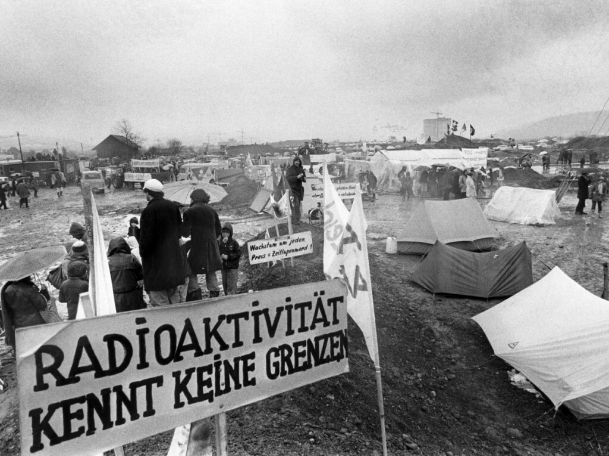
\includegraphics[width=0.75\linewidth]{images/kaiseraugst_1975.png}
\end{center}

\subsection{Politische Verhandlungen}

Ein fünfter Faktor war die politische Bearbeitung
von Umweltfragen.

Einzelne Themen wurden bereits seit den 1950er Jahren
in nationaler und regionaler Politik aufgegriffen.

Dazu gehörten:

\begin{itemize}
\item Langzeitwirkungen atomarer Tests
\item Luftverschmutzung
\item Gewässerschutz
\item gesellschaftliche Leistungen des Waldes
\item Natur- und Artenschutz
\end{itemize}

Zunehmend wurden Umweltfragen
auch international verhandelt.

Ein wichtiger Meilenstein war
die erste Umweltkonferenz in Stockholm 1972.

Dort wurde deutlich,
dass globale Umweltpolitik
unterschiedliche Interessen
miteinander vereinbaren muss.

Vertreterinnen und Vertreter
von Ländern der südlichen Hemisphäre
wehrten sich dagegen,
die gleichen Kosten zu tragen
wie die industrialisierten Länder des Nordens.

Denn diese seien historisch
in viel grösserem Ausmass
für Umweltprobleme verantwortlich.

Auch die Ölkrisen von 1973 und 1979
bildeten einen wichtigen Kontext
für die Umweltdebatte.

\subsection{Umwelt machen}

Die Vorlesung betont,
dass „Umwelt“ nicht einfach
eine natürliche Gegebenheit ist.

Über „Umwelt“ im heutigen Sinn
begann man erst in der zweiten Hälfte
des 20. Jahrhunderts zu sprechen.

Der Begriff existierte zwar bereits seit etwa 1800.

Seine Bedeutung veränderte sich jedoch stark.

Zunächst bedeutete Umwelt
vor allem Umgebung des Menschen.

Später wurde der Begriff
in der Gesellschaftstheorie
als Übersetzung von Milieu verwendet.

Im biologischen Sinn verstand Jakob von Uexküll
unter Umwelt die für ein Lebewesen relevante Umgebung,
die auf seine Lebensbedingungen einwirkt.

Erst um 1970 wurde Umwelt
zum Standardbegriff der ökologischen Bewegung.

Von nun an stand Umwelt
für Natur,
aber auch für Dinge,
Lebewesen,
Vorgänge
und Zusammenhänge,
die in Kontakt und Wechselbeziehung
zum Menschen stehen.

\subsection{Von Natur zu Umwelt}

Vor der modernen Umweltbewegung
sprach man eher von Natur
oder Naturschutz.

Natur wurde dabei häufig
als Gegenbegriff zur Kultur verstanden.

Naturschutz zielte oft auf den Schutz
besonderer Landschaften,
Arten
oder Naturdenkmäler.

Der moderne Umweltbegriff
geht darüber hinaus.

Er beschreibt nicht mehr eine Natur,
die ausserhalb der Gesellschaft steht.

Vielmehr macht er sichtbar,
dass Natur und Kultur
in modernen Gesellschaften
nicht mehr klar voneinander getrennt werden können.

Industrie,
Landwirtschaft,
Chemie,
Verkehr,
Konsum
und Energieversorgung
verändern ökologische Zusammenhänge.

Die zentrale These lautet daher:

Umwelt entsteht historisch dort,
wo die Ununterscheidbarkeit
zwischen Natur und Kultur
in der postmodernen Gesellschaft
sichtbar wird.

\subsection{Historische Antworten auf Umweltprobleme}

Die Vorlesung unterscheidet verschiedene Antworten
auf umweltpolitische Herausforderungen.

Eine erste Antwort ist technische Innovation.

Technologien sollen Probleme lösen,
die selbst technisch oder industriell verursacht wurden.

Produktionsprozesse sollen verbessert,
Schadstoffe reduziert
oder neue Energieformen entwickelt werden.

Diese Strategie kann jedoch
die Komplexität technischer Systeme weiter erhöhen.

Dadurch können neue Abhängigkeiten
und neue Risiken entstehen.

Eine zweite Antwort ist Bevölkerungsregulierung.

Diese ist problematisch,
weil sie zwangsläufig die Frage aufwirft,
wer angeblich „zu viel“ ist.

Historisch zeigt sich dies etwa
an westlich geförderter Geburtenkontrolle
in Indien und China in den 1960er Jahren.

Eine dritte Antwort sind Regulierungen für die Industrie.

Verursacher von Umweltverschmutzung
sollen zur Verantwortung gezogen
und finanziell belastet werden.

Dies ist jedoch schwierig,
weil Industrie politisch gut organisiert ist
und globale Produktions-
und Distributionsprozesse
Verantwortung schwer zuordnen lassen.

Eine vierte Antwort ist die Kommodifizierung von CO2.

Seit den internationalen Klimaverhandlungen
und dem Emissionshandel
werden Umweltprobleme teilweise
in kapitalistische Marktlogiken integriert.

Dadurch wird über Emissionen gehandelt,
anstatt den Wachstumsimperativ selbst
grundsätzlich in Frage zu stellen.

\subsection{Zentrale Erkenntnisse}

Die Vorlesung zeigt,
dass Umweltkatastrophen
und Umweltbewusstsein
eng mit der Geschichte moderner Technik verbunden sind.

Technische Systeme erzeugen nicht nur Fortschritt,
sondern auch Risiken,
Nebenfolgen
und neue Formen politischer Verantwortung.

Zentrale Erkenntnisse sind:

\begin{itemize}
\item Umweltkatastrophen entstehen häufig aus komplexen technischen und organisatorischen Zusammenhängen.
\item In eng gekoppelten Systemen können kleine Störungen zu grossen Krisen eskalieren.
\item Schleichende Umweltkrisen unterscheiden sich stark von plötzlichen Katastrophenereignissen.
\item Umwelt wurde erst im 20. Jahrhundert zu einem zentralen gesellschaftspolitischen Problem.
\item Medien, Wissenschaft, Protestbewegungen und Politik trugen zur Entstehung modernen Umweltbewusstseins bei.
\item Der Begriff Umwelt zeigt, dass Natur und Kultur in modernen Gesellschaften nicht mehr klar trennbar sind.
\item Antworten auf Umweltprobleme bleiben umstritten, weil sie technische, politische, wirtschaftliche und globale Interessen berühren.
\end{itemize}

Die zentrale These lautet:

Umweltprobleme sind keine äusseren Störungen
einer ansonsten funktionierenden technischen Moderne.

Sie sind Teil dieser Moderne selbst.

Die technisierte,
industrialisierte
und wachstumsorientierte Gesellschaft
bringt jene Umweltkrisen hervor,
die sie anschliessend wissenschaftlich,
technisch,
politisch
und gesellschaftlich zu bewältigen versucht.

        \section{Technik und Territorium: Was Infrastrukturen leisten}

\subsection{Einführung: Infrastruktur als technikgeschichtliches Problem}

Die Vorlesung untersucht,
welche Rolle Infrastrukturen für moderne Gesellschaften spielen.

Im Zentrum steht die Frage,
wie technische Netze,
Verkehrssysteme,
Versorgungssysteme
und digitale Infrastrukturen
Räume erschliessen,
Macht organisieren
und gesellschaftlichen Alltag prägen.

Infrastrukturen sind dabei nicht nur technische Einrichtungen.

Sie sind auch politische,
soziale,
ökonomische
und territoriale Ordnungen.

Sie legen fest,
wer Zugang zu bestimmten Räumen,
Ressourcen
und Möglichkeiten erhält.

Zentrale Leitfragen:

\begin{itemize}
\item Was sind Infrastrukturen?
\item Wie erschliessen Infrastrukturen Territorien?
\item Welche Rolle spielen sie für Macht und Herrschaft?
\item Wie prägen Infrastrukturen Alltag und gesellschaftliche Normalität?
\item Worauf baut die digitale Welt materiell und territorial auf?
\end{itemize}

Die Geschichte der Infrastruktur ist daher
nicht nur eine Geschichte von Brücken,
Strassen,
Kanälen,
Eisenbahnen
oder Rechenzentren.

Sie ist auch eine Geschichte davon,
wie Gesellschaften räumlich,
politisch
und technisch geordnet werden.

\subsection{Nachtrag: Umwelt als gesellschaftspolitisches Thema}

Zu Beginn der Sitzung wurde nochmals
an die vorherige Vorlesung
zu Umweltkatastrophen und Umweltbewusstsein angeknüpft.

Umwelt entstand als gesellschaftspolitisches Thema
seit den 1960er Jahren
aus einer Kombination verschiedener Entwicklungen.

Dazu gehörten:

\begin{itemize}
\item populärwissenschaftliche Bücher und Filme
\item das Fernsehen als Medium in privaten Wohnzimmern
\item wissenschaftliche Warnungen und Risikomodelle
\item Katastrophen als Medienereignisse
\item zivilgesellschaftliche Partizipation
\item Anti-AKW-Bewegungen
\item politische Debatten
\end{itemize}

Die 1970er und 1980er Jahre
können daher als Anfang unserer Gegenwart verstanden werden.

Viele heutige Themen,
unter anderem die Umweltfrage,
nahmen in dieser Zeit ihre moderne Form an.

\subsection{Umwelt machen}

Der Begriff „Umwelt“
existiert zwar bereits seit etwa 1800.

Seine heutige Bedeutung erhielt er jedoch erst
im Zuge der Umweltbewegung der 1970er Jahre.

Zuvor sprach man eher von Natur
oder Naturschutz.

Natur wurde dabei häufig als Gegenbegriff
zur Kultur verstanden.

Der moderne Umweltbegriff unterscheidet sich davon.

Er beschreibt nicht einfach eine Natur,
die ausserhalb der Gesellschaft liegt.

Vielmehr bezeichnet er Dinge,
Lebewesen,
Vorgänge
und Zusammenhänge,
die in Kontakt und Wechselbeziehung
zum Menschen stehen.

Umweltpolitik entsteht daher
als Reaktion auf die Wirkungen
industrieller Produktion
und modernen Konsums.

Die zentrale These lautet:

Umwelt entsteht historisch dort,
wo die Ununterscheidbarkeit
zwischen Natur und Kultur
in der postmodernen Gesellschaft sichtbar wird.

\subsection{Antworten auf Umweltprobleme}

Die Vorlesung fasst nochmals
verschiedene historische Antworten
auf umweltpolitische Herausforderungen zusammen.

Eine erste Antwort ist technische Innovation.

Technologien sollen Probleme lösen,
die selbst technisch verursacht wurden.

Produktionsprozesse sollen verbessert,
Emissionen reduziert
oder neue Systeme entwickelt werden.

Dabei entsteht jedoch häufig neue Komplexität.

Eine zweite Antwort ist Bevölkerungsregulierung.

Diese ist problematisch,
weil sie die Frage aufwirft,
wer angeblich zu viel ist
und wer darüber entscheidet,
welche Bevölkerung reguliert werden soll.

Eine dritte Antwort sind Regulierungen für die Industrie.

Verursacher von Umweltverschmutzung
sollen zur Verantwortung gezogen
und finanziell belastet werden.

Dies ist jedoch schwierig,
weil Industrie politisch gut organisiert ist
und globale Produktionsketten
Verantwortung schwer zuordnen lassen.

Eine vierte Antwort ist die Kommodifizierung von CO2.

Durch globalen Emissionshandel
werden Umweltprobleme
in kapitalistische Marktlogiken integriert.

Allen diesen Antworten ist gemeinsam,
dass sie meist darauf verzichten,
wirtschaftliches Wachstum grundsätzlich zu begrenzen
oder den Lebensstandard zu senken.

\subsection{Infrastrukturgeschichte}

Infrastrukturen sind schwer zu fassen.

Betrachtet man sie zu konkret,
besteht die Gefahr,
sich in technischer Dokumentation
und Detailfragen zu verlieren.

Betrachtet man sie zu abstrakt,
werden sie zu Modellen,
in denen nicht mehr klar sichtbar ist,
welche Dinge warum auftauchen
oder unsichtbar bleiben.

Infrastrukturgeschichte fragt daher nicht nur,
wie einzelne technische Systeme funktionieren.

Sie fragt,
was Infrastrukturen gesellschaftlich leisten.

Lange Zeit dienten Infrastrukturprojekte
dem Nation Building,
der Raumerschliessung,
der Machtausübung
und der Demonstration von Überlegenheit.

Solche Funktionen lassen sich seit der Antike beobachten.

Seit dem 19. Jahrhundert
wurden Infrastrukturen besonders wichtig
für moderne Nationalstaaten.

Seit den 1960er Jahren
wurde Infrastruktur zunehmend
als Aufgabe des Staates
und als politische Forderung
der Gesellschaft verstanden.

Auch der Begriff Infrastruktur
etablierte sich in dieser Zeit stärker.

\begin{center}
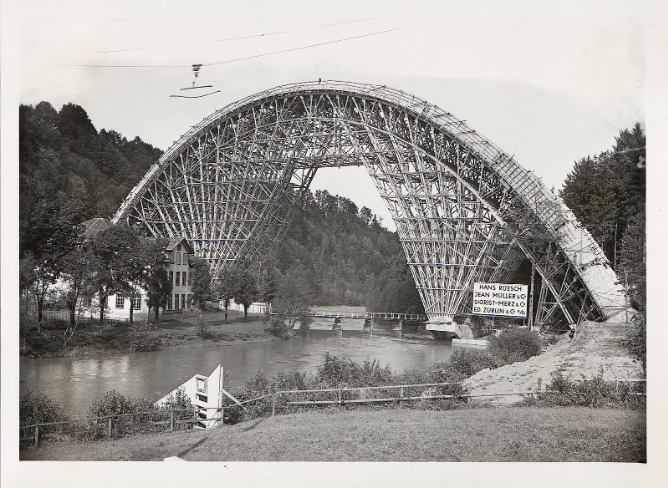
\includegraphics[width=0.75\linewidth]{images/infrastrukturgeschichte_bruecke.png}
\end{center}

\subsection{Was braucht es für funktionierenden Flugverkehr?}

Die Vorlesung zeigt am Beispiel des Flugverkehrs,
dass Technik nie isoliert funktioniert.

Ein Flugzeug allein reicht nicht,
damit Flugverkehr möglich wird.

Notwendig ist ein grosses Netz
aus technischen,
sozialen,
ökonomischen
und politischen Voraussetzungen.

Für funktionierenden Flugverkehr braucht es unter anderem:

\begin{itemize}
\item Orte zum Starten und Landen
\item technische Systeme zur Navigation und Kommunikation
\item Energie- und Treibstoffversorgung
\item Menschen zur Steuerung, Wartung und Koordination
\item Ausbildungs- und Wissenssysteme
\item Verwaltung, Regeln und internationale Abkommen
\item Sicherheits- und Kontrollsysteme
\item digitale Systeme zur Buchung und Organisation
\item globale Liefer- und Wartungsketten
\item Wetter-, Karten- und Informationssysteme
\item Kapital und wirtschaftliche Organisation
\item staatliche und internationale Institutionen
\item Verkehrsanbindungen zum Flughafen
\item Vertrauen in das Funktionieren aller Teilsysteme
\item Passagiere
\end{itemize}

Flugverkehr zeigt daher exemplarisch,
dass moderne Technik
auf Infrastrukturen angewiesen ist.

Technische Systeme funktionieren nur,
wenn viele weitere Systeme
gleichzeitig funktionieren.

\subsection{Strukturelle Bedingungen von Infrastruktur}

Infrastrukturen beruhen auf mehreren
strukturellen Bedingungen.

Erstens funktionieren sie als Netzwerke.

Technik ist Teil eines grösseren Netzes
aus Orten,
Menschen,
Energie,
Wissen
und Kommunikation.

Zweitens benötigen Infrastrukturen Koordination.

Unterschiedliche Akteure,
Institutionen
und technische Systeme
müssen aufeinander abgestimmt werden.

Drittens brauchen Infrastrukturen Standardisierung.

Gemeinsame Regeln,
Normen
und Verfahren
machen Anschlussfähigkeit
überhaupt erst möglich.

Ohne Standardisierung
könnten technische Systeme
nicht dauerhaft,
räumlich übergreifend
und gesellschaftlich verlässlich funktionieren.

\subsection{Infrastruktur als Teil „moderner“ Kulturen}

Infrastrukturen sind kein ausschliesslich modernes Phänomen.

Bereits alte Gesellschaften
bauten technische Systeme,
um Räume zu erschliessen,
Macht auszuüben
und Versorgung zu sichern.

Beispiele dafür sind:

\begin{itemize}
\item der chinesische Kaiserkanal
\item antike Wasserleitungen
\item das römische Strassensystem
\item das Strassensystem der Inka
\end{itemize}

Der chinesische Kaiserkanal
erschloss die Peripherie
mit dem Zentrum.

Das Strassennetz der Inka
erstreckte sich über den Westen Südamerikas
und ermöglichte die administrative Erschliessung
des Imperiums.

Wasserleitungen in Petra
machten einen Ort in der Wüste
überhaupt erst zu einem Macht-
und Wirtschaftszentrum.

Infrastrukturen sind daher
immer auch Mittel,
um Territorien nutzbar,
regierbar
und symbolisch bedeutungsvoll zu machen.

\begin{center}
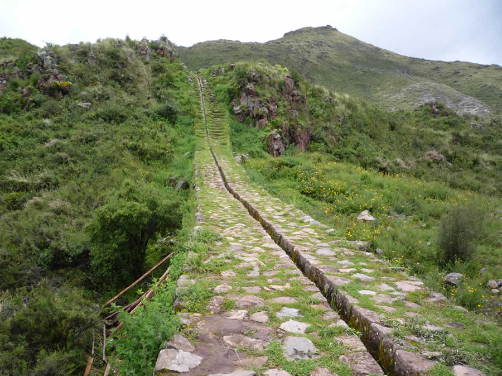
\includegraphics[width=0.85\linewidth]{images/infrastruktur_alte_kulturen.png}
\end{center}

\subsection{Infrastruktur und Modernität}

Modernität ist keine objektive Eigenschaft,
sondern eine Zuschreibung.

Infrastrukturen gelten häufig
als Zeichen von Modernität.

Sie zeigen,
dass gesellschaftliches Zusammenleben
organisiert,
geplant
und technisch unterstützt wird.

Gleichzeitig sollen Infrastrukturen
Modernität auch demonstrieren.

Grosse Brücken,
Kanäle,
Eisenbahnen,
Flughäfen
oder digitale Netze
können als Beweise technischer,
staatlicher
oder wirtschaftlicher Leistungsfähigkeit auftreten.

Infrastrukturen demonstrieren dadurch
auch Überlegenheit.

Sie zeigen,
wer planen,
bauen,
verbinden
und kontrollieren kann.

\subsection{Infrastruktur und Macht}

Infrastrukturen stehen in engem Zusammenhang
mit Macht.

Sie erschliessen und durchdringen Raum.

Strassen,
Kanäle
und Wegesysteme
machen Territorien zugänglich,
begehbar
und administrierbar.

Infrastrukturen können Machtzentren
überhaupt erst hervorbringen.

Aquädukte,
Wasserleitungen
oder Verkehrswege
machen manche Orte
erst zu Herrschafts-
und Handelszentren.

Zugleich vernetzen Infrastrukturen
Machtzentren mit Peripherien.

Sie verbinden administrative,
religiöse
und militärische Zentren
mit entfernten Regionen.

Dadurch ermöglichen sie staatliche Kohärenz
über grosse Räume hinweg.

Infrastrukturen sind auch Kommunikationssysteme.

Strassen,
Kanäle
und Wege dienen nicht nur dem Transport,
sondern auch der Übermittlung von Nachrichten,
Befehlen
und Informationen.

Sie ermöglichen Steuererhebung,
Truppenbewegung,
Versorgung
und damit die praktische Durchsetzung
politischer Ordnung.

\subsection{Kafka und die Chinesische Mauer}

Die Vorlesung bezieht sich auf Franz Kafkas Text
\emph{Beim Bau der Chinesischen Mauer} von 1917.

Darin wird die Chinesische Mauer
nicht nur als Schutzbauwerk betrachtet,
sondern als Projekt,
das über Jahrzehnte und Jahrhunderte
Arbeiterinnen und Arbeiter
aus dem ganzen Reich zusammenführt.

Die Mauer soll vor den „Nordvölkern“ schützen.

In weiten Teilen des Reiches,
etwa im Süden,
sind diese Nordvölker jedoch gar nicht bekannt.

Sie stellen dort keine unmittelbare Bedrohung dar.

Als Feind-
und Bedrohungsbild entstehen sie
erst durch das Bauprojekt selbst.

Kafka zeigt damit,
dass Infrastruktur nicht nur
auf bestehende politische Ordnung reagiert.

Sie bringt politische Ordnung
auch hervor.

Der Bau der Mauer beweist
der peripheren Bevölkerung,
dass es einen Kaiser,
ein Kaiserreich,
eine Dynastie
und damit ein chinesisches Reich gibt.

Infrastruktur stiftet also Zugehörigkeit,
auch dort,
wo die Machtzentrale
im Alltag kaum erfahrbar ist.

\subsection{Infrastruktur und Territorium}

Am Beispiel der Chinesischen Mauer wird sichtbar,
dass Infrastruktur Territorium erst herstellt.

Ein Reich ist nicht einfach dadurch gegeben,
dass es auf einer Karte existiert.

Es muss praktisch,
symbolisch
und materiell erfahrbar gemacht werden.

Grossprojekte wie Mauern,
Kanäle,
Strassen
oder Eisenbahnen
verbinden entfernte Regionen
mit einem politischen Zentrum.

Sie machen Macht sichtbar.

Sie schaffen Orientierung,
Zugehörigkeit
und Kontrollmöglichkeiten.

Territorium ist daher nicht nur Fläche.

Territorium entsteht durch Infrastrukturen,
die Raum erschliessen,
ordnen
und in politische Herrschaft übersetzen.

\subsection{Kongokonferenz in Berlin 1884}

Ein weiteres Beispiel für den Zusammenhang
von Infrastruktur,
Territorium
und Macht
ist die Kongokonferenz in Berlin 1884.

Dort trafen sich europäische Mächte
unter der Leitung von Otto von Bismarck.

Ziel war es,
Regeln für die koloniale Expansion in Afrika festzulegen
und Konflikte zwischen europäischen Staaten zu vermeiden.

Ein zentrales Prinzip war
die sogenannte „effektive Okkupation“.

Territoriale Ansprüche galten nur dann,
wenn tatsächliche Kontrolle ausgeübt wurde.

Dies beschleunigte den kolonialen Wettbewerb
um Afrika,
den sogenannten \emph{Scramble for Africa}.

Infrastruktur wurde dadurch
zum Beweis staatlicher Herrschaft.

Wer Strassen,
Bahnlinien,
Telegrafie
und Verwaltungszentren errichtete,
konnte territoriale Ansprüche legitimieren.

\begin{center}
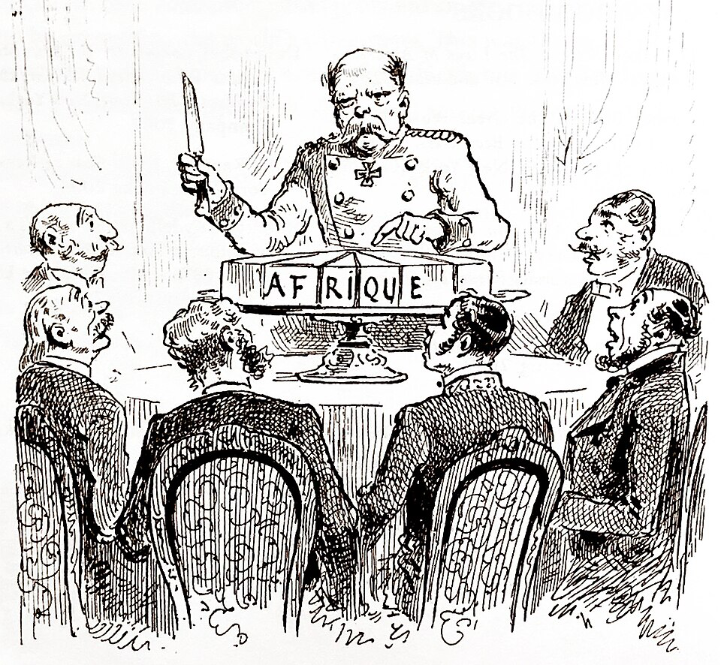
\includegraphics[width=0.75\linewidth]{images/kongokonferenz_berlin_1884.png}
\end{center}

\subsection{Infrastruktur als imperiale Strategie}

Koloniale Infrastruktur diente selten
primär der lokalen Entwicklung.

Zwar wurde Kolonialismus häufig damit gerechtfertigt,
dass koloniale Gebiete zivilisiert
und modern gemacht würden.

Tatsächlich wurde Infrastruktur jedoch vor allem
für imperiale Zwecke aufgebaut.

Dazu gehörten:

\begin{itemize}
\item militärische Mobilität
\item Rohstoffexport
\item Steuererhebung
\item Kommunikation zwischen Küste und Inland
\item Sichtbarmachung staatlicher Macht
\end{itemize}

Wer über Infrastruktur nachdenkt,
muss daher fragen:

\begin{itemize}
\item Wer baut?
\item Wer finanziert?
\item Wer betreibt?
\item Wer nutzt?
\item Wem nützt die Infrastruktur?
\end{itemize}

Infrastruktur war und ist nicht bloss Technik.

Sie ist ein Mittel,
Territorien überhaupt erst
als regierbare Räume hervorzubringen.

\subsection{Postkoloniale Infrastruktur}

Auch nach der Unabhängigkeit
einst kolonisierter Staaten
blieben Infrastrukturen politisch bedeutsam.

Sie konnten weiterhin eine Möglichkeit
zur Einflussnahme
für ehemalige Kolonialmächte darstellen.

Dies verweist auf postkoloniale Machtverhältnisse.

Ein Beispiel ist die Kenya and Uganda Railroad.

Sie führte vom Landesinnern
zu den Handelsstädten an der Küste.

Solche Infrastrukturen waren häufig
auf koloniale Interessen ausgerichtet.

Sie verbanden Rohstoffgebiete
mit Häfen,
Verwaltungszentren
und imperialen Handelswegen.

Für lokale Bevölkerungen bedeuteten sie nicht unbedingt
eine gleichmässige Erschliessung
oder Verbesserung der Lebensbedingungen.

Vielmehr ordneten sie Räume
nach kolonialen Interessen.

\begin{center}
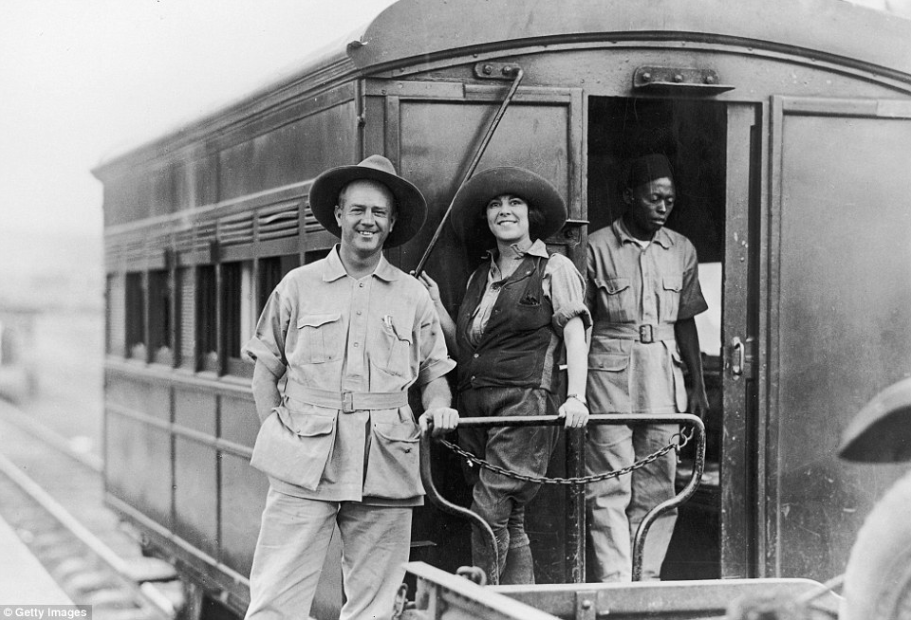
\includegraphics[width=0.75\linewidth]{images/kenya_uganda_railroad.png}
\end{center}

\subsection{Normativität und Alltag}

Im Verlauf des 20. Jahrhunderts
wurden immer mehr Menschen
auf infrastrukturelle Leistungen angewiesen.

Sie kamen regelmässig
mit Infrastrukturen in Kontakt.

Dazu gehören unter anderem:

\begin{itemize}
\item öffentlicher Verkehr
\item Spitäler
\item Stromversorgung
\item Kommunikation
\item Wasser
\item Internet
\end{itemize}

Infrastrukturen organisieren nicht nur Versorgung
und Mobilität.

Sie prägen auch,
wie Menschen leben,
handeln
und denken.

Sie legen fest,
was als normal
oder selbstverständlich erscheint.

Das Stromnetz erzeugt zum Beispiel
die Erwartung dauerhafter Verfügbarkeit
von Licht,
Arbeit
und elektrischen Geräten.

Autogerechte Städte machen das Auto
zur dominanten Mobilitätsform
und prägen das Erscheinungsbild
von Städten und Landschaften.

Infrastrukturen lenken Verhalten.

Sie machen bestimmte Handlungen einfach
und andere schwierig.

Ihre normative Kraft fällt meist erst dann auf,
wenn sie ausfallen.

Wenn Strom,
Wasser,
Internet
oder Verkehrssysteme nicht funktionieren,
wird sichtbar,
wie abhängig der Alltag
von Infrastruktur ist.

\subsection{Infrastruktur als materialisierte gesellschaftliche Ordnung}

Seit spätestens der zweiten Hälfte
des 20. Jahrhunderts
ist Infrastruktur materialisierte
gesellschaftliche Ordnung.

Sie organisiert gesellschaftliches Zusammenleben
und prägt individuellen Alltag.

Infrastrukturen sind daher nicht neutral.

Sie enthalten Vorstellungen davon,
wie Menschen leben sollen,
wie Räume genutzt werden sollen
und welche Formen von Mobilität,
Kommunikation
oder Versorgung selbstverständlich sind.

Das Beispiel der tiefen Brücken
von Robert Moses auf Long Island zeigt dies besonders deutlich.

Die Brücken waren zu niedrig
für Fahrzeuge des öffentlichen Verkehrs.

Dadurch wurde der Zugang zu bestimmten Parks
faktisch Menschen mit PKW vorbehalten.

Infrastruktur konnte somit soziale Ungleichheit
und Ausschluss materiell festschreiben.

Technische Gestaltung
wurde zu sozialer Ordnung.

\subsection{Worauf baut unsere digitale Welt?}

Die Vorlesung fragt abschliessend,
worauf die digitale Welt eigentlich baut.

Digitale Räume erscheinen häufig immateriell
oder virtuell.

Tatsächlich beruhen sie jedoch
auf umfangreichen materiellen Infrastrukturen.

Dazu gehören:

\begin{itemize}
\item Rechenzentren
\item Glasfasernetze
\item Unterseekabel
\item Stromversorgung
\item Kühlung
\item Plattformarchitekturen
\item Datenprotokolle
\item seltene Erden
\item Arbeitskräfte
\item Lieferketten
\end{itemize}

Auch die digitale Welt hat daher
eine territoriale Grundlage.

Sie benötigt Orte,
Energie,
Rohstoffe,
Gebäude,
Netzwerke
und politische Rahmenbedingungen.

Wichtige Fragen lauten:

\begin{itemize}
\item Was ist die Infrastruktur des Digitalen?
\item Wer betreibt sie?
\item Wo befindet sie sich?
\item Wer zahlt?
\item Wer baut sie auf?
\item Wer nutzt sie?
\end{itemize}

\subsection{Virtualität und Territorium}

Digitale Infrastrukturen sind eng
mit anderen Infrastrukturen verbunden.

Kommunikation,
Militär,
Mobilität,
Industrie,
Finanzmarkt,
Logistik
und Bildung
sind zunehmend auf digitale Systeme angewiesen.

Gleichzeitig bauen digitale Infrastrukturen
auf älteren Infrastrukturen auf.

Schon immer wurden Infrastrukturen
auf andere Infrastrukturen aufgebaut.

Kommunikation und Transport
waren beispielsweise historisch eng verbunden.

Auch Rechenzentren
sind nicht einfach virtuelle Räume.

Sie brauchen Strom,
Kühlung,
Gebäude,
Sicherheit,
Netzanbindung
und politische Regulierung.

Die digitale Infrastruktur wirkt daher territorial,
ähnlich wie frühere Infrastrukturen
wie das Strassennetz der Inka,
der chinesische Kaiserkanal,
Eisenbahnen
oder Brücken.

Sie ordnet Räume,
schafft Abhängigkeiten,
ermöglicht Kontrolle
und verbindet Zentren mit Peripherien.

\begin{center}
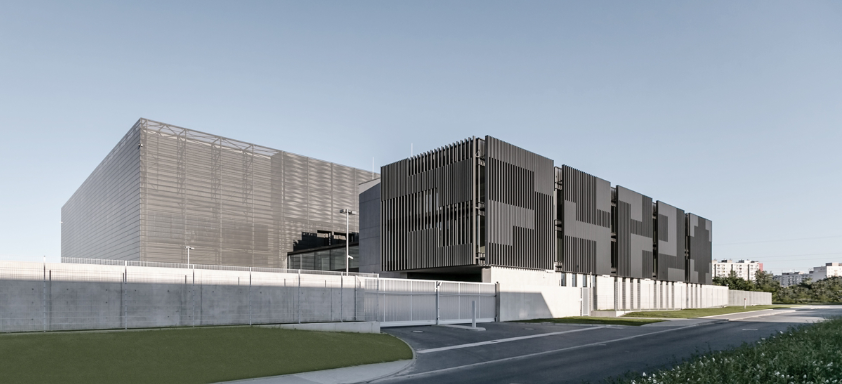
\includegraphics[width=0.75\linewidth]{images/data_center_poznan.png}
\end{center}

\subsection{Zentrale Erkenntnisse}

Die Vorlesung zeigt,
dass Infrastrukturen weit mehr leisten
als technische Versorgung.

Sie erschliessen Räume,
organisieren Gesellschaft,
stabilisieren Macht
und prägen Alltag.

Zentrale Erkenntnisse sind:

\begin{itemize}
\item Infrastrukturen funktionieren als Netzwerke aus Technik, Menschen, Energie, Wissen und Institutionen.
\item Sie benötigen Koordination und Standardisierung.
\item Infrastrukturprojekte dienten historisch der Raumerschliessung, Machtausübung und Demonstration von Modernität.
\item Infrastrukturen machen Territorien zugänglich, administrierbar und regierbar.
\item Koloniale Infrastruktur diente häufig imperialen Interessen statt lokaler Entwicklung.
\item Infrastrukturen prägen Alltag, Normalität und Verhalten.
\item Digitale Welten beruhen auf materiellen und territorialen Infrastrukturen.
\end{itemize}

Die zentrale These lautet:

Infrastruktur ist nicht bloss technische Grundlage
gesellschaftlichen Lebens.

Sie ist materialisierte Ordnung.

Sie schafft Räume,
regelt Zugang,
organisiert Macht
und macht Gesellschaften
in bestimmter Weise handlungsfähig.

Wer Infrastrukturen baut,
kontrolliert oder nutzt,
gestaltet daher nicht nur Technik,
sondern auch Territorium,
Alltag
und gesellschaftliche Möglichkeiten.

        \section{Langzeitwirkung: Die Erzählung der De-Industrialisierung und das Leben im Anthropozän}

\subsection{Einführung: De-Industrialisierung und Langzeitwirkungen}

Die Vorlesung untersucht die Erzählung
der De-Industrialisierung
und verbindet sie mit der Frage,
wie technische Systeme langfristig
soziale,
räumliche
und ökologische Wirkungen entfalten.

Im Zentrum steht nicht nur die Frage,
ob Industrie verschwindet.

Entscheidend ist vielmehr,
was von industriellen Gesellschaften bleibt,
wenn Fabriken,
Zechen
oder industrielle Arbeitsplätze geschlossen werden.

De-Industrialisierung bedeutet daher nicht einfach
das Ende der Industrie.

Sie beschreibt vielmehr eine Verschiebung
industrieller Produktion,
die Auflösung bestimmter sozialer Ordnungen
und das Nachleben technischer Systeme.

Zentrale Leitfragen:

\begin{itemize}
\item Was bedeutet De-Industrialisierung?
\item Warum erscheint seit den 1970er Jahren das Ende der Industriegesellschaft plausibel?
\item Welche Rolle spielen Angestellte, Automatisierung, Globalisierung und Neoliberalismus?
\item Was bleibt von Industrie nach ihrer Stilllegung?
\item Wie wirken technische Systeme im Anthropozän langfristig weiter?
\end{itemize}

Die Vorlesung zeigt,
dass industrielle Technik nicht einfach endet,
wenn industrielle Arbeit verschwindet.

Ihre Spuren bleiben in Landschaften,
Infrastrukturen,
sozialen Milieus,
politischen Konflikten
und ökologischen Belastungen erhalten.

\subsection{Ölschiefer-Abbau im Nordosten Estlands}

Ein zentrales Beispiel der Vorlesung
ist der Ölschiefer-Abbau im Nordosten Estlands.

Die Region um Kiviõli
war seit den 1920er Jahren
eine wichtige Industrieregion,
besonders während der Sowjetzeit.

Ölschiefer ist ein Gestein,
das organisches Material namens Kerogen enthält.

Dieses entstand vor Millionen von Jahren
aus abgestorbenen Algen und Mikroorganismen.

Durch Verschwelung kann aus Ölschiefer
Öl gewonnen werden.

Dazu wird das Gestein abgebaut,
zerkleinert
und unter Sauerstoffausschluss stark erhitzt.

Typischerweise geschieht dies bei Temperaturen
von etwa 450 bis 500 Grad Celsius.

Dabei zerfällt das Kerogen chemisch.

Es entstehen:

\begin{itemize}
\item flüssige Kohlenwasserstoffe
\item Schieferöl
\item brennbare Gase
\item Rückstände aus Kohlenstoff und Mineralien
\end{itemize}

Die Dämpfe werden anschliessend abgekühlt,
sodass ein rohes Öl entsteht,
das ähnlich wie Erdöl weiter raffiniert werden kann.

\subsection{Industrialisierung, Sowjetzeit und sozialer Umbruch}

Der Ölschiefer-Abbau machte den Nordosten Estlands
zu einer zentralen Industrieregion.

Während der Sowjetzeit
wurden viele russischsprachige Arbeiterinnen und Arbeiter
in der Region angesiedelt.

Die industrielle Struktur
prägte daher nicht nur die Wirtschaft,
sondern auch Bevölkerung,
Sprache,
Arbeitswelt
und regionale Identität.

Nach dem Zusammenbruch der Sowjetunion um 1990
kam es zu einem tiefgreifenden Strukturwandel.

Die sowjetischen Absatz-
und Versorgungsstrukturen brachen zusammen.

Es folgten Rationalisierung,
Schliessungen
und Arbeitsplatzverluste.

Die Region erlebte einen raschen sozialen
und demographischen Rückgang.

De-Industrialisierung bedeutete hier also nicht nur,
dass bestimmte Produktionsformen verschwanden.

Sie bedeutete auch den Verlust
einer sozialen Ordnung,
die auf industrieller Arbeit,
staatlicher Planung
und regionaler Zugehörigkeit beruhte.

\begin{center}
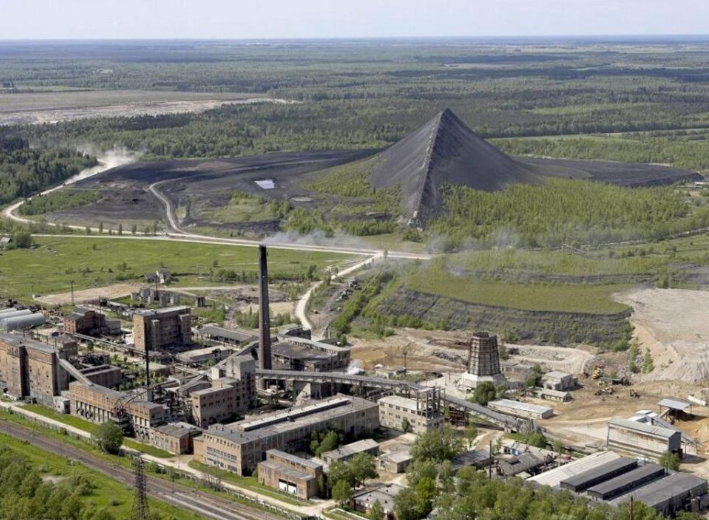
\includegraphics[width=0.8\linewidth]{images/oelschiefer_estland.png}
\end{center}

\subsection{Industrie als Nachleben}

Die Landschaft im Nordosten Estlands
bleibt bis heute industriell geprägt.

Auch wenn industrielle Produktion zurückgeht
oder sich verändert,
verschwinden ihre Spuren nicht.

Zurück bleiben:

\begin{itemize}
\item Gruben
\item Kraftwerke
\item industrielle Infrastrukturen
\item Abraumhalden
\item belastete Böden
\item transformierte Landschaften
\end{itemize}

Das Kiviõli Adventure Center
steht exemplarisch für dieses industrielle Nachleben.

Es befindet sich auf einem Berg
aus Abfällen der Ölschieferindustrie.

Dieser Berg glüht in seinem Innern
weiterhin auf rund 80 Grad Celsius.

Die frühere Industrielandschaft
wird nun touristisch genutzt,
etwa durch Freizeitparks,
Abenteuerferien
und Veranstaltungsorte.

Solche Nutzungen können als Industriearchäologie
oder als Versuch verstanden werden,
wirtschaftliche Alternativen aufzubauen.

Gleichzeitig bleiben soziale
und wirtschaftliche Fragilität bestehen.

Die Industrie ist daher nicht einfach abgeschlossen.

Sie lebt als Landschaft,
Infrastruktur,
Risiko
und Erinnerung weiter.

\begin{center}
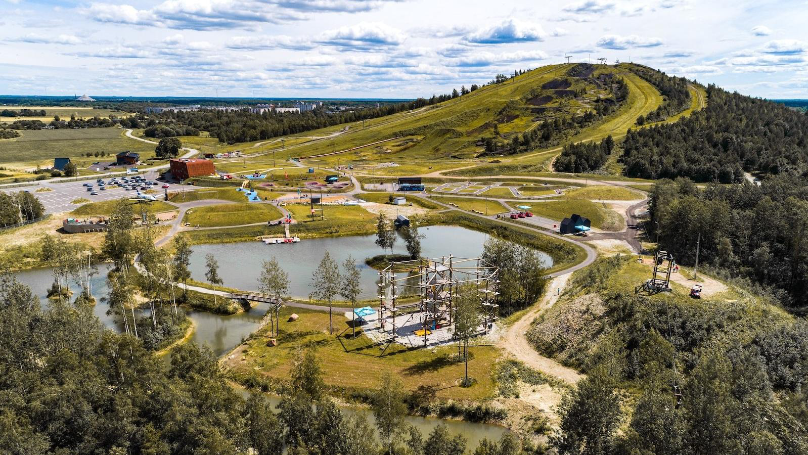
\includegraphics[width=0.8\linewidth]{images/kivioli_adventure_center.png}
\end{center}

\subsection{Das Ende der Industriegesellschaft?}

Seit den 1970er Jahren
entstand in westlichen Gesellschaften
zunehmend der Eindruck,
das industrielle Zeitalter gehe zu Ende.

Mehrere Entwicklungen schienen
auf einen Übergang
in eine neue Gesellschaftsform hinzuweisen.

Dazu gehörten:

\begin{itemize}
\item Rückgang klassischer Industriearbeit
\item Bedeutungsverlust der klassischen Arbeiterklasse
\item Schliessung von Zechen und Fabriken
\item Wachstum des Dienstleistungssektors
\item Wachstum von Verwaltung, Finanzwirtschaft und Bildung
\item Aufstieg von Informationstechnologie
\item Zunahme von Angestellten- und Wissensarbeit
\end{itemize}

Die westlichen Gesellschaften schienen
in ein postindustrielles,
wissensbasiertes
oder informationsbasiertes Zeitalter einzutreten.

Begriffe wie Wissensgesellschaft,
Informationsgesellschaft
oder Netzwerkgesellschaft
wurden Ausdruck dieser Erwartung.

Technische Entwicklungen wie Automatisierung,
politische Entwicklungen wie Neoliberalismus
und sozioökonomische Entwicklungen wie Globalisierung
verstärkten diesen Eindruck.

\subsection{De-Industrialisierung als Erzählung}

De-Industrialisierung bezeichnet
nicht nur konkrete historische Entwicklungen.

Sie ist auch eine gesellschaftliche Erzählung.

Diese Erzählung wurde durch öffentliche Diskussionen
in unterschiedliche Richtungen gedeutet.

Einerseits gab es eine euphorische Deutung.

Das Ende der Schwerindustrie
wurde als Übergang
in ein neues,
modernes
und scheinbar sauberes Zeitalter verstanden.

Industrie erschien dabei als alt,
schmutzig
und überholt.

Informationstechnologie,
Dienstleistungsarbeit
und Wissensarbeit galten dagegen
als Zukunft.

Andererseits gab es eine pessimistische Deutung.

Hier erschien De-Industrialisierung
als soziale Krise.

Im Zentrum standen:

\begin{itemize}
\item Verlust von Arbeit
\item Verlust von Identität
\item Bedeutungsverlust ganzer Regionen
\item Arbeitslosigkeit
\item politische Entfremdung
\item soziale Verarmung
\end{itemize}

Die Erzählung der De-Industrialisierung
war daher ambivalent.

Sie konnte Fortschritt versprechen,
aber auch Niedergang,
Verlust
und Krise bedeuten.

\subsection{Die Angestellten als Produkt der Industrialisierung}

Ein wichtiger Teil dieser Geschichte
ist die Entstehung des modernen Angestelltentums.

Angestellte entstanden nicht erst
nach der Industriegesellschaft.

Sie sind selbst ein Produkt
der Industrialisierung des 19. Jahrhunderts.

Mit wachsender industrieller Produktion
entstanden neue Anforderungen
an Verwaltung,
Planung,
Buchhaltung,
Kommunikation
und technische Koordination.

Grosse Unternehmen,
Eisenbahnen,
Banken,
Versicherungen
und Staatsverwaltungen
benötigten zunehmend Personal,
das nicht direkt an der Maschine arbeitete.

Diese Personen organisierten,
verwalteten
und koordinierten industrielle Prozesse.

Das Angestelltentum war daher
eng mit der Industriegesellschaft verbunden,
auch wenn es sich häufig
von der Arbeiterschaft abgrenzte.

\subsection{Technisierung des Büros}

Das moderne Angestelltentum entstand
zusammen mit neuen Technologien
der Informationsverarbeitung.

Dazu gehörten:

\begin{itemize}
\item Schreibmaschinen
\item Telefone
\item Karteisysteme
\item Rechenmaschinen
\item standardisierte Formulare
\item später Computer und Datenverarbeitung
\end{itemize}

Die industrielle Produktion
musste nicht nur hergestellt,
sondern auch geplant,
verwaltet
und koordiniert werden.

Dafür brauchte es bürokratische Bereiche.

Diese umfassten etwa:

\begin{itemize}
\item Korrespondenz mit Kunden
\item Kontakt zu Abnehmern und Verkäufern
\item Handel und Vertrieb
\item Statistik
\item Marktbeobachtung
\item Produktionsplanung
\end{itemize}

Die Anpassungsfähigkeit der Produktion
wurde zunehmend marktrelevant.

Dafür brauchte es Überblick,
eingespielte Verfahren
und Informationsverarbeitung.

Das Büro war daher kein Gegensatz
zur Industrie.

Es war eine Voraussetzung
für deren komplexe Organisation.

\subsection{Identität und Zugehörigkeit der Angestellten}

Angestellte waren zwar lohnabhängig,
verstanden sich historisch jedoch häufig
nicht als Teil der Arbeiterschaft.

Sie entwickelten eigene Selbstbilder
und soziale Abgrenzungen.

Typische Selbstbilder waren:

\begin{itemize}
\item geistige statt körperliche Arbeit
\item Bildung und Respektabilität
\item Individualität
\item Aufstiegsorientierung
\item Nähe zu Verwaltung, Technik und Management
\end{itemize}

Sozial grenzten sich Angestellte
häufig nach unten
von der Arbeiterschaft ab.

Gleichzeitig orientierten sie sich nach oben
an bürgerlichen Lebensformen.

Dadurch verkomplizierte das Angestelltentum
den klassischen Gegensatz
zwischen Bourgeoisie und Proletariat.

Gesellschaftliche Konflikte
liessen sich nicht mehr nur
als Klassenkampf zwischen Arbeiterschaft
und Besitzbürgertum beschreiben.

\begin{center}
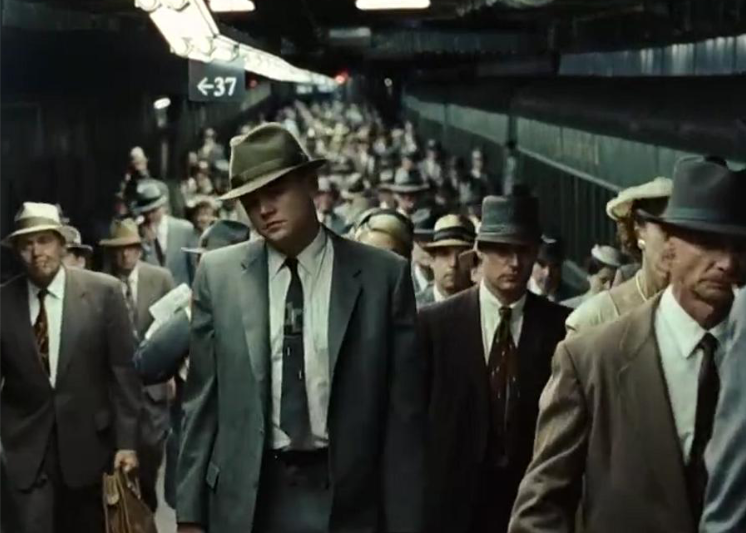
\includegraphics[width=0.75\linewidth]{images/angestellte_identitaet.png}
\end{center}

\subsection{Angestellte und De-Industrialisierung}

Die Orientierung des Angestelltentums
hatte Auswirkungen auf das politische
und gesellschaftliche Gefüge.

Sie trug dazu bei,
bürgerliche Lebensstile
über die eigentliche bürgerliche Bevölkerungsschicht hinaus
zu verbreiten.

In den 1970er Jahren
lösten Angestellte die Arbeiterschaft
jedoch nicht einfach als soziale Gruppe ab.

Vielmehr verschob sich die symbolische Bedeutung.

Während der Industriearbeiter lange
als zentrale Figur moderner Produktion galt,
erschienen seit den 1970er Jahren
zunehmend Angestellte,
Verwaltungsarbeiter
und Wissensarbeiter
als repräsentativ für die Zukunft
westlicher Gesellschaften.

Der Angestellte erschien nun
als geeigneter Träger
einer neuen Wirtschaftsordnung.

Diese schien weniger auf sichtbare,
körperliche Produktion ausgerichtet zu sein
als auf Organisation,
Kommunikation
und Informationsverarbeitung.

\subsection{Automatisierung und Computerisierung}

Computerisierung und Automatisierung
veränderten industrielle Produktionsprozesse
grundlegend.

Tätigkeiten wurden standardisiert,
technisch reorganisiert
und datenbasiert koordiniert.

Industriearbeit verschwand dadurch jedoch nicht einfach.

Computer ersetzten den Industriearbeiter
oder die Industriearbeiterin nicht vollständig.

Sie veränderten vielmehr,
welche Fähigkeiten
und Qualifikationen
erforderlich wurden.

Bestimmte Formen industrieller Arbeit
verloren an Bedeutung,
während neue technische,
organisatorische
und kontrollierende Tätigkeiten wichtiger wurden.

Automatisierung bedeutete daher
nicht das Ende von Arbeit,
sondern ihre Neuordnung.

\subsection{Globalisierung und räumliche Entkopplung}

Neben der Automatisierung spielte
die Globalisierung eine zentrale Rolle.

Produktion wurde zunehmend global organisiert.

Unternehmen verlagerten:

\begin{itemize}
\item Fertigung
\item Rohstoffgewinnung
\item Montage
\item Zulieferketten
\item arbeitsintensive Produktionsschritte
\end{itemize}

Dadurch entstand eine politische Konkurrenz
zwischen Staaten.

Diese konkurrierten etwa um:

\begin{itemize}
\item niedrige Steuern
\item günstige Arbeitsbedingungen
\item schwächere Regulierungen
\item geringere Umweltauflagen
\end{itemize}

Die Folge war die De-Industrialisierung
vieler westlicher Industrieregionen.

Klassische Industriearbeitsplätze gingen verloren.

Zugleich wurden Konsum,
Verwaltung
und Produktion räumlich voneinander getrennt.

Industrie verschwand dadurch nicht an sich.

Sie verschwand vor allem
aus dem unmittelbaren Blickfeld
westlicher Gesellschaften.

\subsection{Die neoliberale Wende}

Ein weiterer wichtiger Faktor
war die neoliberale Wende.

Nach 1945 entstand in vielen westlichen Staaten
eine Form sozialstaatlich regulierten Kapitalismus.

Diese beruhte auf:

\begin{itemize}
\item Massenproduktion
\item Massenkonsum
\item Tarifpartnerschaft
\item relativ stabiler Industriearbeit
\item sozialstaatlicher Absicherung
\end{itemize}

Die Industriegesellschaft wurde politisch stabilisiert.

Dies geschah nicht nur aus ökonomischen Gründen.

Es ging auch darum,
sozialen Frieden zu sichern.

Wichtige Hintergründe waren:

\begin{itemize}
\item die Erinnerung an Faschismus und Weltwirtschaftskrise
\item die Stärke der Gewerkschaften
\item die Vermeidung von Klassenkampf
\item der Kalte Krieg und die Konkurrenz zum Staatssozialismus
\end{itemize}

Industriepolitik war damit auch Gesellschaftspolitik.

Sie versprach Vollbeschäftigung,
regionale Stabilität
und politische Befriedung.

\subsection{Auflösung des Nachkriegsarrangements}

Das Nachkriegsarrangement
zwischen Arbeitgeberinnen,
Arbeitgebern,
Arbeitnehmerinnen
und Arbeitnehmern
bedeutete eine künstliche Stabilisierung
industrieller Gesellschaften.

In den 1970er Jahren
wurde dieses Arrangement zunehmend in Frage gestellt.

Gründe dafür waren unter anderem:

\begin{itemize}
\item Ölkrisen
\item zunehmende internationale Konkurrenz
\item Automatisierung
\item Globalisierung
\item Arbeitslosigkeit
\item Finanzialisierung
\end{itemize}

Globalisierung reduzierte lokale Abhängigkeiten.

Technische Umstrukturierung
veränderte Produktionsweisen.

Arbeitslosigkeit schwächte Gewerkschaften.

Finanzialisierung veränderte Unternehmenslogiken.

Die wirtschaftlichen und politischen Bedingungen
veränderten sich so,
dass der soziale Kompromiss der Nachkriegszeit
zunehmend aufgekündigt wurde.

Besonders deutlich wurde dies
in Thatchers Grossbritannien
und Reagans USA.

\subsection{Britische Bergarbeiterstreiks 1984/85}

Ein zentrales Beispiel für die neoliberale Wende
sind die britischen Bergarbeiterstreiks
von 1984 und 1985.

Die Regierung Thatcher wollte
unrentable Zechen schliessen
und Subventionen abbauen.

Damit verband sie auch das Ziel,
die Macht der Gewerkschaften
in der britischen Politik zu brechen.

Die Wirtschaft sollte grundlegend umgebaut werden.

Dieser Umbau richtete sich gegen
das sozialstaatlich stabilisierte
Nachkriegsarrangement.

Als Thatcher 1984
die Schliessung zahlreicher Zechen beschloss,
traten mehr als 150 000 Bergarbeiter
für fast ein Jahr in den Streik.

Organisiert wurde der Streik
von der National Union of Mineworkers.

Es handelte sich um den grössten Arbeiterstreik
der britischen Nachkriegszeit.

\begin{center}
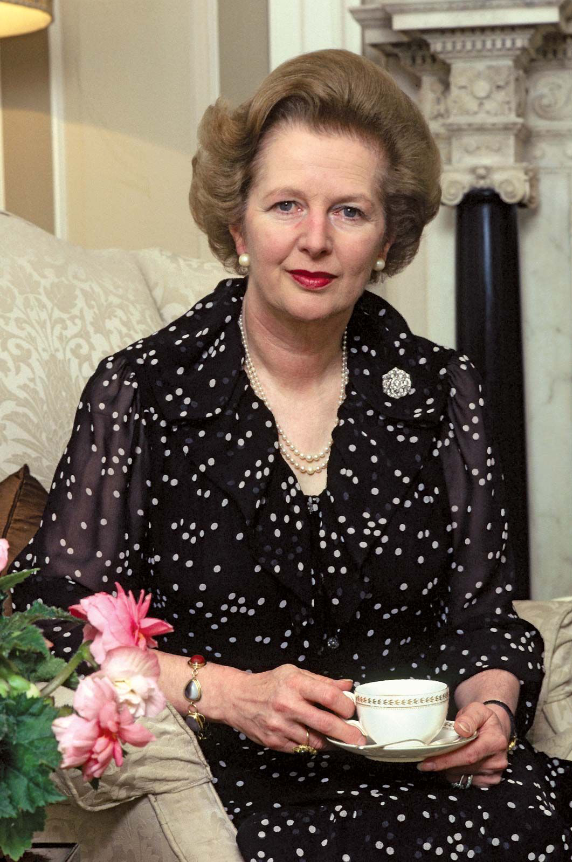
\includegraphics[width=0.75\linewidth]{images/thatcher_bergarbeiterstreik.png}
\end{center}

\subsection{Der Bergarbeiterstreik als Kampf um Lebensformen}

Der Kohlebergbau hatte in Regionen
wie Yorkshire,
Wales,
den Midlands,
Nordengland
und Schottland
eine Bedeutung,
die weit über die reine Wirtschaft hinausging.

Er prägte:

\begin{itemize}
\item lokale Gemeinschaften
\item Geschäfte
\item politische Identitäten
\item Wohnungsbau
\item Gewerkschaftskulturen
\item regionale Zugehörigkeit
\end{itemize}

Die Bergarbeiter verstanden den Konflikt
daher nicht nur als Arbeitskampf.

Sie sahen ihn als Kampf
um Lebensformen,
um das Überleben ganzer Industriestandorte,
um regionale Gemeinschaften
und um politische Würde.

Der Streik endete jedoch
mit einer Niederlage der Bergarbeiter.

Viele Zechen wurden geschlossen.

Die Macht der Gewerkschaften
brach massiv ein.

Auch die Überzeugung,
dass die lokale Arbeiterschaft nötig sei,
um die Wirtschaft am Laufen zu halten,
wurde geschwächt.

\subsection{Langzeitfolgen der De-Industrialisierung}

Langfristig beschleunigte die Niederlage
der britischen Bergarbeiter
die De-Industrialisierung
vieler Industrieregionen.

Die Folgen waren tiefgreifend.

Dazu gehörten:

\begin{itemize}
\item Massenarbeitslosigkeit
\item soziale Verarmung
\item politische Entfremdung
\item langfristige regionale Ungleichheit
\item schlechte Infrastruktur
\item Gesundheitsprobleme
\item politische Radikalisierung
\item Perspektivlosigkeit
\end{itemize}

Diese Folgen verschwanden nicht
nach wenigen Jahren.

Viele ehemalige Bergbauregionen
kämpfen bis heute
mit den strukturellen Nachwirkungen
der De-Industrialisierung.

Damit wird deutlich,
dass De-Industrialisierung
nicht nur ein ökonomischer Prozess ist.

Sie verändert soziale Welten
und wirkt über Generationen weiter.

\begin{center}

\includegraphics[width=0.75\linewidth]{images/bergarbeiterstreik_1984_85.png}
\end{center}

\subsection{Mehr als De-Industrialisierung}

Was seit den 1970er Jahren geschah,
war in gewissem Sinne mehr
als De-Industrialisierung.

Denn es verschwanden nicht nur Arbeitsplätze.

Es verschwanden ganze soziale Welten.

Dazu gehörten:

\begin{itemize}
\item industrielle Identitäten
\item kollektive Lebensformen
\item regionale Zugehörigkeiten
\item politische Milieus
\item Gewerkschaften und Arbeiterbewegung
\item Zukunftserwartungen
\item kulturelle Selbstverständnisse
\end{itemize}

Nicht nur Arbeit verschwand,
sondern die industrielle Gesellschaft
als Erfahrungsraum.

Industrie war also nicht nur
eine Produktionsform.

Sie war auch eine soziale,
politische
und kulturelle Ordnung.

\subsection{Weniger als De-Industrialisierung}

Gleichzeitig war der Prozess
auch weniger als De-Industrialisierung.

Denn Industrie verschwand nicht einfach.

Industriepolitik gibt es weiterhin.

Auch heute existieren etwa
Autoindustrie,
Stahlindustrie,
Gewerkschaften,
Tarifverträge
und Verhandlungen zwischen Sozialpartnern.

Was sich veränderte,
war vor allem die räumliche,
soziale
und politische Konzentration der Industrie.

Produktion wurde verlagert,
Prozesse wurden automatisiert
und Wertschöpfungsketten wurden fragmentiert.

Industrie verschwand also nicht,
sondern wurde räumlich entkoppelt
und verlor an Sichtbarkeit.

De-Industrialisierung bezeichnet daher
weniger das Ende der Industrie
als die Auflösung ihrer lokalen,
sozialen
und politischen Konzentration.

\subsection{Leben im Anthropozän}

Die Vorlesung verbindet De-Industrialisierung
mit der Frage nach dem Leben im Anthropozän.

Das Anthropozän bezeichnet eine Gegenwart,
in der menschliche Eingriffe
geologische,
ökologische
und planetare Wirkung entfalten.

Technische Systeme prägen dabei
nicht nur unmittelbare Arbeitsprozesse.

Sie wirken langfristig weiter.

Wichtige Aspekte sind:

\begin{itemize}
\item normative Wirkung technischer Systeme
\item Irreversibilität technischer Eingriffe
\item Trägheit materieller Infrastrukturen
\item langfristige ökologische Folgen
\item Transformation von Landschaften
\item Veränderung von Stoffkreisläufen
\item soziale und kulturelle Nachwirkungen
\end{itemize}

Technik strukturiert Arbeit,
Verhalten
und Wahrnehmung
über ihre reine Funktion hinaus.

Sie prägt Alltagsroutinen,
Organisationen
und Erwartungen.

\subsection{Langzeitwirkung technischer Systeme}

Technische Systeme enden nicht
mit den Gesellschaften,
die sie hervorgebracht haben.

Ihre Wirkungen können ihre ursprünglichen
sozialen,
politischen
und ökonomischen Kontexte überdauern.

Industrieanlagen,
Infrastrukturen,
Bergwerke,
Abraumhalden
und belastete Landschaften
wirken weiter,
auch wenn die ursprüngliche Produktion
eingestellt wurde.

Solche Systeme sind träge.

Sie lassen sich nicht einfach abschalten
oder rückgängig machen.

Ihre Folgen können Generationen überdauern.

Das gilt sozial,
räumlich
und ökologisch.

Wenn man über De-Industrialisierung nachdenkt,
wird daher klar:

Industrie verschwindet nicht einfach.

Sie bleibt als Nachleben,
als Infrastruktur,
als ökologische Belastung,
als soziale Erinnerung
und als politische Folge bestehen.

\subsection{Zentrale Erkenntnisse}

Die Vorlesung zeigt,
dass De-Industrialisierung
nicht einfach das Ende der Industrie bedeutet.

Sie beschreibt vielmehr die Verschiebung
und Entkopplung industrieller Produktion
sowie den Verlust bestimmter sozialer,
politischer
und regionaler Ordnungen.

Zentrale Erkenntnisse sind:

\begin{itemize}
\item Industrie wirkt auch nach ihrer Stilllegung weiter.
\item De-Industrialisierung bedeutet nicht das vollständige Verschwinden von Industrie.
\item Industrie verliert vor allem ihre lokale, soziale und politische Konzentration.
\item Angestellte und Wissensarbeit entstehen selbst aus der Industrialisierung.
\item Automatisierung verändert Arbeit, ersetzt sie aber nicht einfach vollständig.
\item Globalisierung verschiebt Produktion aus dem Blickfeld westlicher Gesellschaften.
\item Die neoliberale Wende löste das Nachkriegsarrangement industrieller Stabilisierung auf.
\item De-Industrialisierung betrifft nicht nur Arbeitsplätze, sondern ganze Lebensformen.
\item Technische Systeme entfalten langfristige soziale, räumliche und ökologische Wirkungen.
\end{itemize}

Die zentrale These lautet:

De-Industrialisierung ist weniger das Ende der Industrie
als die Auflösung ihrer sichtbaren,
lokalen
und gesellschaftlich stabilisierten Form.

Industrie verschwindet nicht einfach.

Sie wird verlagert,
automatisiert,
fragmentiert
und bleibt zugleich als Nachleben bestehen.

Im Anthropozän zeigt sich,
dass technische Systeme
nicht mit ihren historischen Gesellschaften enden,
sondern als langfristige Strukturen weiterwirken.

        \section{Prüfungsvorbereitung: Musterfragen}

\subsection{Frage 1: Was sind Zünfte?}

\textbf{Fragestellung}

Worum handelt es sich bei den Zünften?

\textbf{Antwort}

Zünfte waren Zusammenschlüsse von Handwerkern im Mittelalter und in der Frühen Neuzeit.

Sie regelten:

\begin{itemize}
\item Ausbildung von Lehrlingen
\item Qualitätsstandards
\item wirtschaftliche Interessen
\item Zugang zu bestimmten Berufen
\end{itemize}

Ziel war die Kontrolle handwerklicher Produktion sowie die Sicherung der wirtschaftlichen Stellung ihrer Mitglieder.

\subsection{Frage 2: Weshalb scheiterte Fords Kautschukprojekt im Amazonas?}

\textbf{Fragestellung}

Warum wollte Henry Ford eine eigene Kautschukplantage errichten und weshalb scheiterte das Vorhaben?

\textbf{Antwort}

Ford benötigte grosse Mengen Kautschuk für die Reifenproduktion seiner Automobile. Durch eine eigene Plantage wollte er sich vom internationalen und kolonial geprägten Kautschukhandel unabhängig machen.

Das Projekt scheiterte jedoch aus mehreren Gründen:

\begin{itemize}
\item mangelndes Wissen über tropische Landwirtschaft
\item ungeeignete Managemententscheidungen
\item Krankheiten und Probleme beim Kautschukanbau
\item Widerstand der lokalen Bevölkerung gegen die vorgegebenen Arbeits- und Lebensweisen
\end{itemize}

Das Beispiel zeigt die Grenzen technischer und wirtschaftlicher Planung in fremden ökologischen und sozialen Kontexten.

\subsection{Frage 3: Warum wurde Umwelt in den 1970er Jahren zum Politikum?}

\textbf{Fragestellung}

Welche Faktoren führten dazu, dass Umweltfragen in den 1970er Jahren politisch wichtig wurden?

\textbf{Antwort}

Seit den 1960er und 1970er Jahren wurden Umweltprobleme zunehmend öffentlich wahrgenommen.

Wichtige Gründe waren:

\begin{itemize}
\item Berichte über Umweltkatastrophen
\item Fernsehreportagen und Medienberichte
\item populärwissenschaftliche Veröffentlichungen
\item wissenschaftliche Forschung zu Umweltproblemen
\item Entstehung von Umweltbewegungen
\item Proteste gegen technische Grossprojekte wie Kernkraftwerke
\end{itemize}

Dadurch entwickelte sich Umwelt von einem wissenschaftlichen Thema zu einer gesellschaftlichen und politischen Frage.

\subsection{Frage 4: Quellenkritik zur Frankfurter Küche}

\begin{center}
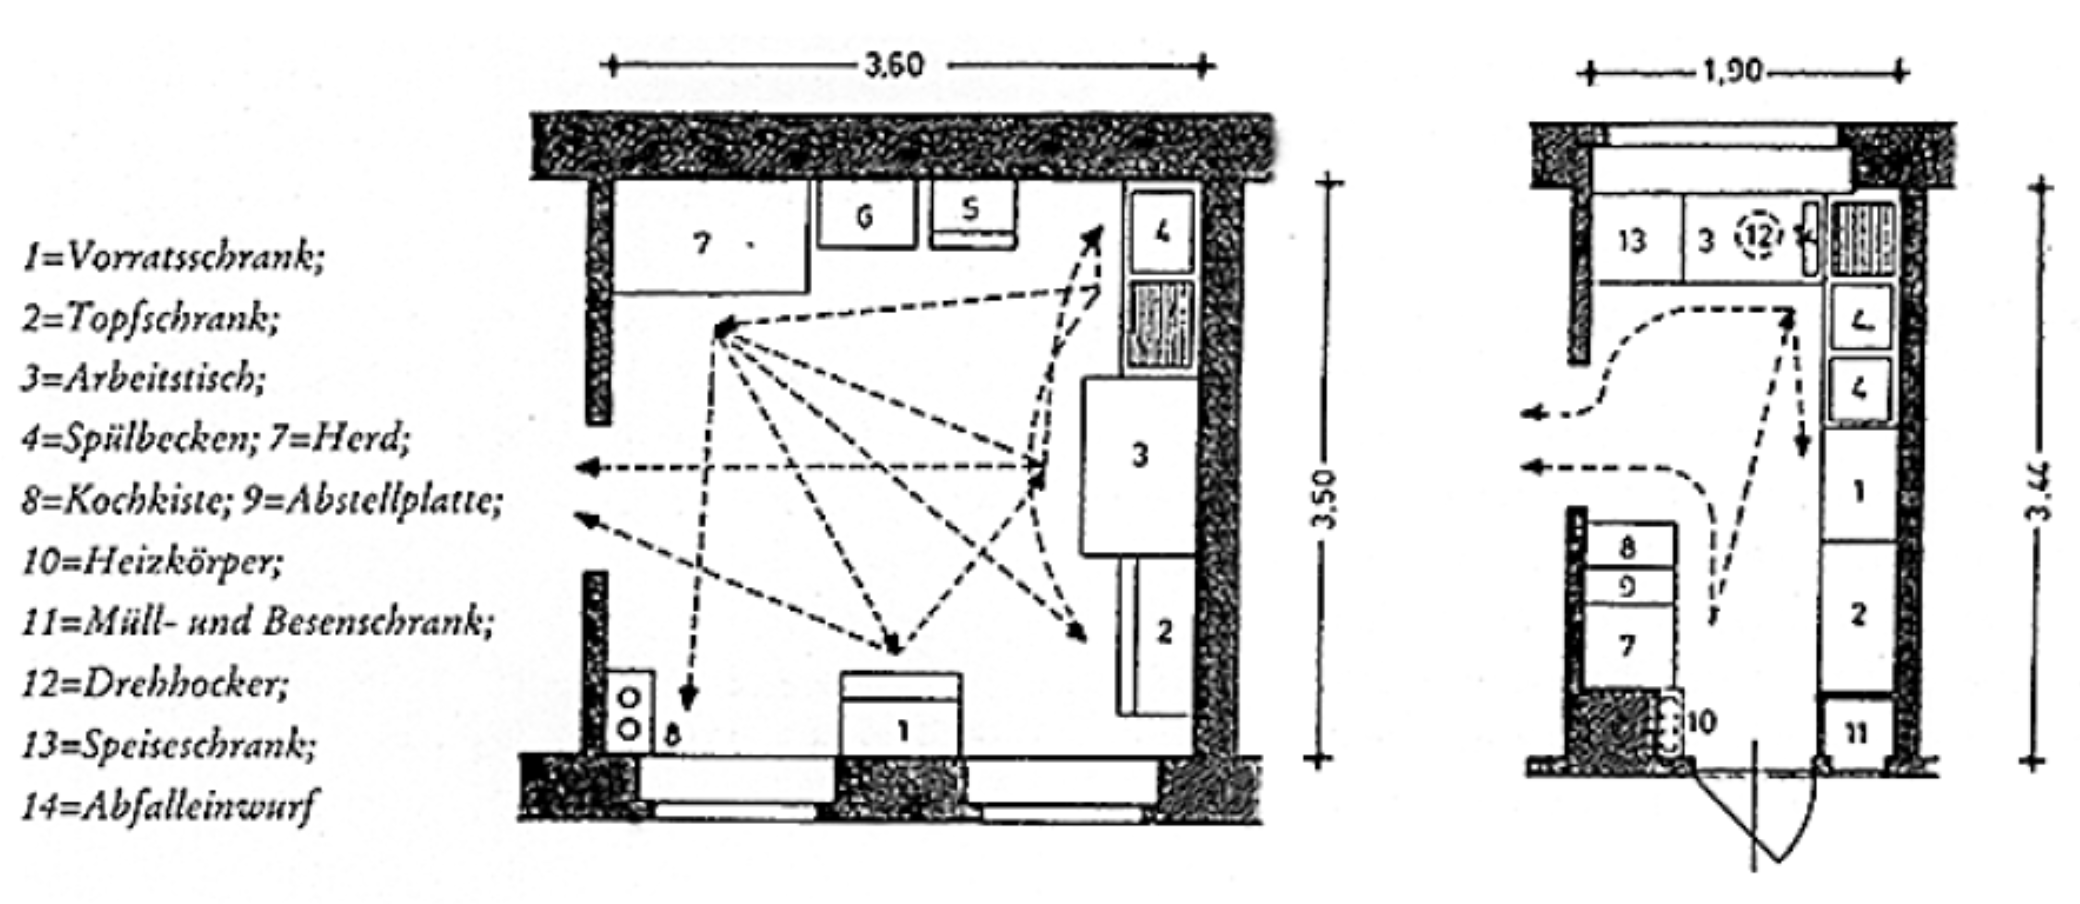
\includegraphics[width=0.8\linewidth]{images/frankfurter_kueche.png}
\end{center}

\textbf{Fragestellung}

Beschreibe Aufbau und Gestaltung der Küche, erläutere die Rationalisierungsprinzipien und interpretiere die Quelle im Hinblick auf moderne Haushaltsführung.

\textbf{Antwort}

Die Frankfurter Küche wurde in den 1920er Jahren entwickelt und sollte Hausarbeit effizienter gestalten.

Herd, Spüle, Arbeitsflächen und Schränke sind so angeordnet, dass Arbeitswege möglichst kurz bleiben. Die Küche ist kompakt, funktional und stark standardisiert.

Die Gestaltung orientiert sich am Scientific Management von Frederick Taylor. Arbeitsabläufe werden analysiert und optimiert, um Zeit und Kraftaufwand zu sparen. Damit werden industrielle Rationalisierungsprinzipien auf den privaten Haushalt übertragen.

Die Quelle zeigt moderne Vorstellungen von Ordnung, Hygiene und Effizienz. Gleichzeitig macht sie deutlich, dass Hausarbeit weiterhin überwiegend Frauen zugewiesen wurde. Die Frankfurter Küche steht daher sowohl für technischen Fortschritt als auch für Standardisierung und Disziplinierung des Alltags.

\subsection{Zentrale Erkenntnisse}

Für die Prüfung besonders wichtig:

\begin{itemize}
\item Zünfte regulierten handwerkliche Arbeit und Ausbildung.
\item Ford wollte Rohstoffe kontrollieren, scheiterte aber an lokalen Bedingungen.
\item Umwelt wurde durch Medien, Wissenschaft und soziale Bewegungen politisiert.
\item Die Frankfurter Küche übertrug industrielle Rationalisierung auf den Haushalt.
\item Technikgeschichte untersucht immer auch soziale, politische und kulturelle Folgen technischer Entwicklungen.
\end{itemize}

    \end{layout}
\end{document}
